\documentclass[journal]{IEEEtran}

\hyphenation{op-tical net-works semi-conduc-tor}
\usepackage{graphicx}
\usepackage[linesnumbered,ruled,vlined]{algorithm2e}
\usepackage{algorithm}
\usepackage{algorithmic}
\usepackage{amsmath}
\usepackage{booktabs}
\usepackage{cite}
\usepackage{bm}
\usepackage{amsfonts}
\usepackage{color,xcolor}
\usepackage{subcaption}
\usepackage{caption}
\usepackage{subfigure}
\usepackage{graphicx}
\usepackage{float}
\usepackage{multirow}
\renewcommand{\thesubfigure}{\alph{subfigure}} 
\usepackage[labelfont=bf]{caption}

\begin{document}

\title{Multi-Balancing-Agent Reinforcement Learning for Charging Control of Lithium-ion Batteries}


\author{Hejiakang~Cao,
        Bing-Chuan~Wang,~\IEEEmembership{Member,~IEEE,}
        Biao Luo,~\IEEEmembership{Senior Member,~IEEE}
        and Zhongmei Li,~\IEEEmembership{Member,~IEEE}
        % <-this % stops a space
        
\thanks{Hejiakang Cao, Bing-Chuan Wang, and Biao Luo are with the School of Automation, Central South University, Changsha 410083, China (e-mail: 8207220713@csu.edu.cn; bingcwang@csu.edu.cn; biao.luo@csu.edu.cn).

Zhongmei Li is with the Key Laboratory of Smart Manufacturing in Energy Chemical Process, Ministry of Education, East China University of Science and Technology, Shanghai 200237, China (e-mail: zhongmeili@ecust.edu.cn).
}% <-this % stops a space
}

%\markboth{Journal of \LaTeX\ Class Files,~Vol.~14, No.~8, August~2015}%
%{Shell \MakeLowercase{\textit{et al.}}: Bare Demo of IEEEtran.cls for IEEE Journals}

\maketitle

% As a general rule, do not put math, special symbols or citations
% in the abstract or keywords.
\begin{abstract}
Efficient and fast charging balancing control of lithium-ion batteries has garnered significant attention in recent years. Traditional charging balancing control methods typically rely on balancing algorithms that operate on equalization topologies, causing varying currents to flow through individual cells to achieve state of charge (SOC) balancing across all cells. However, these methods face several challenges: 1) equalization topologies could reduce charging precision and efficiency; 2) discharging high-SOC cells leads to energy loss; 3) the potential for re-emerging imbalance after initial balancing is frequently overlooked. To address these challenges, this paper introduces a new multi-balancing-agent reinforcement learning (MBA-RL) framework for charging control. In this framework, each agent independently defines a dedicated charging protocol for its respective cell, while coordinating with other agents to achieve SOC balancing across all cells. MBA-RL eliminates the need for equalization topologies and avoids discharging operations on high-SOC cells. It not only facilitates rapid SOC balancing but also supports fast charging under balanced conditions. Experimental results demonstrate that MBA-RL significantly reduces the time required to achieve SOC balancing while optimizing the overall charging process. It outperforms both the single-agent deep Q-learning method and the traditional constant current-constant voltage approach.
\end{abstract}

% Note that keywords are not normally used for peerreview papers.
\begin{IEEEkeywords}
Charging control, SOC balancing, lithium-ion battery, multi-agent reinforcement learning
\end{IEEEkeywords}

\IEEEpeerreviewmaketitle

\section{Introduction}

\IEEEPARstart{L}{ithium-ion} batteries have been extensively adopted in the electric vehicle (EV) industry due to their environment-friendly nature, high energy density, low self-discharge rate, and long cycle life \cite{1, 2}. However, individual lithium-ion batteries are inherently limited in meeting the high voltage and capacity demands required by EVs \cite{3, 4}. As a result, practical energy storage systems are composed of hundreds to thousands of individual battery cells. However, inevitable inconsistencies in manufacturing and operational conditions introduce variations in internal states and lifespan across battery cells, which can significantly compromise a battery pack’s overall capacity, charging efficiency, and durability while also increasing safety risks \cite{5, 6}. Therefore, it is crucial to formulate an efficient and practical charging equalization strategy that reduces charging time under safety constraints while ensuring inter-cell balance within the battery pack. To achieve this objective, researchers have developed numerous equalization strategies. Most of these strategies employ a framework that combines equalization topologies with balancing algorithms, where the balancing algorithm regulates the topology structure to achieve the redistribution of charge and energy within the battery pack \cite{7, 8}. Different balancing algorithms applied to the same equalization topology can yield varying results, and vice versa. A reasonable equalization strategy should strike a balance between these two aspects, taking into account the specific requirements of the application \cite{ma2024two}. A detailed overview of the framework is provided as follows.

\subsubsection*{Equalization topologies}The equalization topologies can be categorized into active equalization topologies and passive equalization topologies. The active equalization topologies involve redistributing excess charge from high-energy cells to those with lower energy levels via switched capacitors, inductors \cite{9}, transformers \cite{10}, or DC-DC converters \cite{11}, thereby facilitating an efficient discharging process for high-energy cells while simultaneously charging low-energy cells. Despite the higher energy utilization efficiency offered by active balancing, designing an effective equalization topology becomes increasingly intricate when managing a large number of cells configured in both series and parallel arrangements. This significantly increases the complexity of the system and the associated design costs. Passive equalization topologies achieve charging equalization by employing discharge resistors connected in parallel with the cells within the battery pack \cite{12}. These resistors serve as a channel for high-energy cells to dissipate excess charge, with the energy being converted into heat during the process. Although the design of passive balancing is relatively straightforward, the dissipation of energy through resistors substantially reduces energy efficiency, leading to significant resource wastage. Additionally,  regardless of whether active or passive equalization topologies are used, discharging higher-SOC cells to achieve faster balancing is unavoidable. This not only reduces energy efficiency but also increases safety risks.

\subsubsection*{Balancing algorithms}Traditional balancing algorithms are typically based on constant current-constant voltage (CC-CV) methods to achieve voltage or SOC balancing among battery cells. Aizpuru {\it et al.} \cite{13} integrated the CC-CV method with single-cell experimental data to construct a passive balancing system. Hoque {\it et al.} \cite{14} applied particle swarm optimization (PSO) to optimize the CC-CV balancing controller, aiming to improve balancing performance. Although CC-CV based balancing algorithms are straightforward to design, they fail to consider temperature variations within the battery pack and rely on overly conservative constraints to mitigate safety risks. With the advancement of control theory, an increasing number of studies have combined control theory with charging equalization topologies. In \cite{15}, a balancing algorithm employing fuzzy logic control was proposed to adaptively manage the equalization process for lithium-ion batteries. Fan {\it et al.} \cite{16} introduced a fast-balancing strategy based on model predictive control to resolve the issue of imbalance among individual cells in lithium-ion battery packs. While these approaches can enhance the precision and efficiency of charging equalization, they still fail to adapt to dynamic changes in battery parameters during the charging process. To address the aforementioned issues, Yang {\it et al.} \cite{17} presented a balancing awareness charging control framework based on deep reinforcement learning (DRL). In \cite{18}, a DRL-based controller was introduced for active equalization of redundant battery systems. These approaches leverage DRL’s adaptability to dynamic environments and its strong exploration capabilities to determine the optimal charging policy. Nevertheless, the previously mentioned DRL methods exhibit several issues: 1) depending on an equalization topology to enable charge and energy redistribution among cells, which compromises both charging efficiency and precision; 2) overlooking the possibility that, despite achieving an initially balanced state, variations in the charging environment may lead to SOC inconsistencies re-emerging in subsequent charging cycles.

% Nevertheless, the previously mentioned methods necessitates the integration of a equalization topology to facilitate energy transfer among cells, thereby compromising both charging efficiency and precision. Furthermore, due to disparities in the initial states of individual cells, these methods inevitably involve discharging certain cells within the battery pack, which diminishes energy utilization efficiency and exacerbates safety risks.

Recently, a novel technique called multi-agent reinforcement learning (MARL) has been introduced \cite{19, 20}. It implements an experience-sharing mechanism among agents while ensuring that each agent independently follows its own policy. This approach accelerates convergence to optimal policies and enhances robustness, making it highly suitable for complex control and decision-making problems. Liang {\it et al.} \cite{21} utilized MARL for real-time management of a battery swapping and charging system. Dong {\it et al.} \cite{22} proposed an MARL mechanism to optimize the peak shaving performance of the electric grid. In a charging balancing control problem, MARL effectively coordinates the fast charging of individual cells with the balancing control requirements across the entire battery pack. This approach eliminates the necessity for traditional equalization topologies, thus simplifying the charging process. However, despite this advantage, MARL has not yet been explored for charging balancing control in battery management systems.

Based on these considerations, this paper proposes a new multi-balancing-agent reinforcement learning (MBA-RL) framework for charging control that operates independently of any specific equalization topology. MBA-RL not only facilitates fast SOC balancing but also ensures sustained SOC balancing within the battery pack throughout subsequent charging cycles. Moreover, we employ a battery pack composed of real battery cells with varying lifespans to validate the effectiveness of MBA-RL, thereby making it more representative of real-world scenarios. The main contributions of this paper are summarized as follows.
\begin{enumerate}
    \item A general MBA-RL charging control framework is proposed, which is adaptable to various MARL algorithms and battery models. Additionally, it eliminates the need for equalization topologies, enhancing both the precision and efficiency of the charging balancing process.
    
    \item MBA-RL provides several substantial advantages. First, it demonstrates exceptional flexibility, enabling the application of different constraints to individual battery cells to meet practical engineering requirements. Second, MBA-RL effectively eliminates the need for discharging actions, thereby optimizing energy utilization and reducing charging costs. Lastly, it ensures rapid SOC balancing across all batteries while simultaneously improving the charging speed under balanced conditions.
    
    \item Unlike most DRL algorithms that are evaluated solely through simulations, this study validates MBA-RL using real battery data with different cycle lifetimes, thereby making the proposed algorithm more realistic and reliable.
\end{enumerate}

The remainder of this paper is structured as follows. The charging balancing problem is briefly revisited in Section II. The proposed MBA-RL framework is detailed in Section III, followed by validation results and discussions in Section IV. Finally, Section V concludes this paper.

\section{Problem Formulation}
First, the electrochemical-thermal model used for charging balancing control is described. Next, the charging balancing control is formulated as a constrained optimization problem.

\subsection{Electrochemical-Thermal Model}
\subsubsection{Electrochemical Model}
The electrochemical model characterizes the electrochemical dynamic behaviors of the lithium-ion battery. Given the efficiency and accuracy of the single particle model (SPM) \cite{23}, it is adopted in our study. Since SPM assumes a uniform distribution of solid-phase and electrolyte potential within the battery, the reaction overpotential and the lithium-ion intercalation/deintercalation rates are consistently homogeneous, allowing a single particle to represent the entire electrode. More details of SPM can be found in \cite{24, 25}. Based on the characteristics of SPM, the voltage can be calculated as:
\begin{equation}\label{eqn:voltage}
    V(t) = U^{ref}_{p} \left( \frac{c_{s,\text{surf},p}(r,t)}{c_{s,\text{max},p}} \right) - U^{ref}_{n} \left( \frac{c_{s,\text{surf},n}(r,t)}{c_{s,\text{max},n}} \right)
\end{equation}
where $t$ is the temporal coordinate, $r$ is the radial coordinate, $U^{ref}_{p}$ and $U^{ref}_{n}$ represent the reference voltages of the positive and negative electrodes, respectively, the terms \(c_{s,\text{surf},p}(r,t)\) and \(c_{s,\text{surf},n}(r,t)\) denote the lithium-ion concentrations at the surfaces of the positive and negative electrodes, respectively, and $c_{s,\text{max},p}$ and $c_{s,\text{max},n}$ indicate the maximum lithium-ion concentrations within the positive and negative electrodes, respectively. Next, the SOC of the battery model can be estimated as follows:
\begin{equation}
 SOC(t)= \frac{\int_{0}^{R_p} c_{s,\text{surf},p}(r,t) \, \text{d}r - C_{\min}}{C_{\max} - C_{\min}}   
\end{equation}
where $C_{\min}$ indicates the lithium-ion concentration in the positive electrode particles at a SOC of 0\%, $C_{\max}$ represents the lithium-ion concentration in the positive electrode particles at a SOC of 100\%, and $R_p$ denotes the thickness of the battery’s positive electrode.

\subsubsection{Thermal Model}
The thermal model describes the thermal dynamics of the battery:
\begin{equation}\label{eqn:thermal}
    \rho c_p \frac{\partial T}{\partial t} = k \nabla^2 T + I (E - V) + IT \frac{\text{d}E}{\text{d}T}
\end{equation}
where $I$ indicates the total current passing through the battery, $T$ represents the battery temperature, $E$ is the equilibrium potential, $\frac{\text{d}E}{\text{d}T}$ denotes the entropy coefficient, $\rho$ stands for the density of the battery material, $c_p$ indicates the specific heat capacity, $k$ represents the thermal conductivity, and $\nabla^2 T$ is the Laplacian operator, which describes the spatial distribution of the battery temperature.


\subsection{Charging Balancing Control Problem}
The objective of charging balancing control is to minimize the time required to reach the terminal conditions, which can be described as follows:
% The objective of charging balancing control is to minimize the time required for the standard deviation $\sigma$ of the initial SOC across all cells in the battery pack $\mathcal{B}$ to remain within a predefined threshold $\beta$, ensuring high consistency. Additionally, it is essential to guarantee that the battery pack reaches the reference SOC $SOC_{ref}$ under these balanced conditions. The aforementioned process can be described as follows:

\begin{equation}\label{eqn:balancing objective}
    \displaystyle \max\limits_{\bm{\mathbb{I}}(t)} \quad - (t_b-t_0) 
\end{equation}
with terminal conditions:
\begin{equation}\label{terminal condition}
    \sigma = \sqrt{\frac{1}{n} \sum_{i=1}^{n} \left(SOC_i(t_b) - \overline{SOC}(t_b)\right)^2} \leq \beta
\end{equation}
\begin{equation}\label{terminal condition}
    SOC_i(t_b) \geq SOC_{ref}, \, i = 1,2,...,n
\end{equation}
where $\bm{\mathbb{I}}(t) = \left[ I_1(t), \dots, I_n(t) \right]^{\mathrm{T}} \in \mathbb{R}^{n}$ represents the vector of currents for $n$ cells in the battery pack at the time step $t$, $t_0$ and $t_b$ correspond to the initial and final times of the charging process, respectively, $\sigma$ denotes the standard deviation of the SOC across all batteries in the battery pack $\mathcal{B}$, $\beta$ specifies the predefined threshold for charging balancing, $SOC_i(t_b)$ denotes the SOC of the $i$-th cell in $\mathcal{B}$ at $t_b$, $\overline{SOC}(t_b)$ indicates the mean SOC of all cells in $\mathcal{B}$ at $t_b$, and $SOC_{ref}$ represents the reference SOC for each cell.

To prevent any cell within the battery pack $\mathcal{B}$ from violating safety and balance constraints, which could diminish the battery pack's lifespan and reduce charging efficiency, the $i$-th cell in $\mathcal{B}$ must comply with the following constraints:

\begin{equation}\label{safty condition}
    \begin{array}{rl}
    & \quad I_{\min} \leq I_i(t) \leq I_{\max} \\[10pt]
    & \quad T_i(t) \leq T_{\max}, \quad V_i(t) \leq V_{\max} \\[10pt]
    % & \quad SOC_{\min} \leq SOC_i(t) \leq SOC_{\max} \\[10pt]
    \end{array}
\end{equation}
where the charging current of each cell $I_i(t)$ is constrained between $I_{\min}$ and $I_{\max}$, and $T_{\max}$ and $V_{\max}$ are the upper limits of temperature and voltage for the $i$-th cell, respectively.

Charging balancing control must ensure the safe and stable charging of individual cells, while also accelerating the SOC balancing process across the entire battery pack. However, there is currently a limited body of research that effectively balance the requirements of both individual cells and the entire battery pack. To fill this gap, this paper proposes an MBA-RL framework for solving the charging balancing control problem, which will be comprehensively discussed in the following section. 

% In this framework, each agent independently establishes a dedicated charging protocol for its respective cell while communicating with other agents to achieve SOC balance across the entire battery pack.

 \begin{figure}
    \centering
    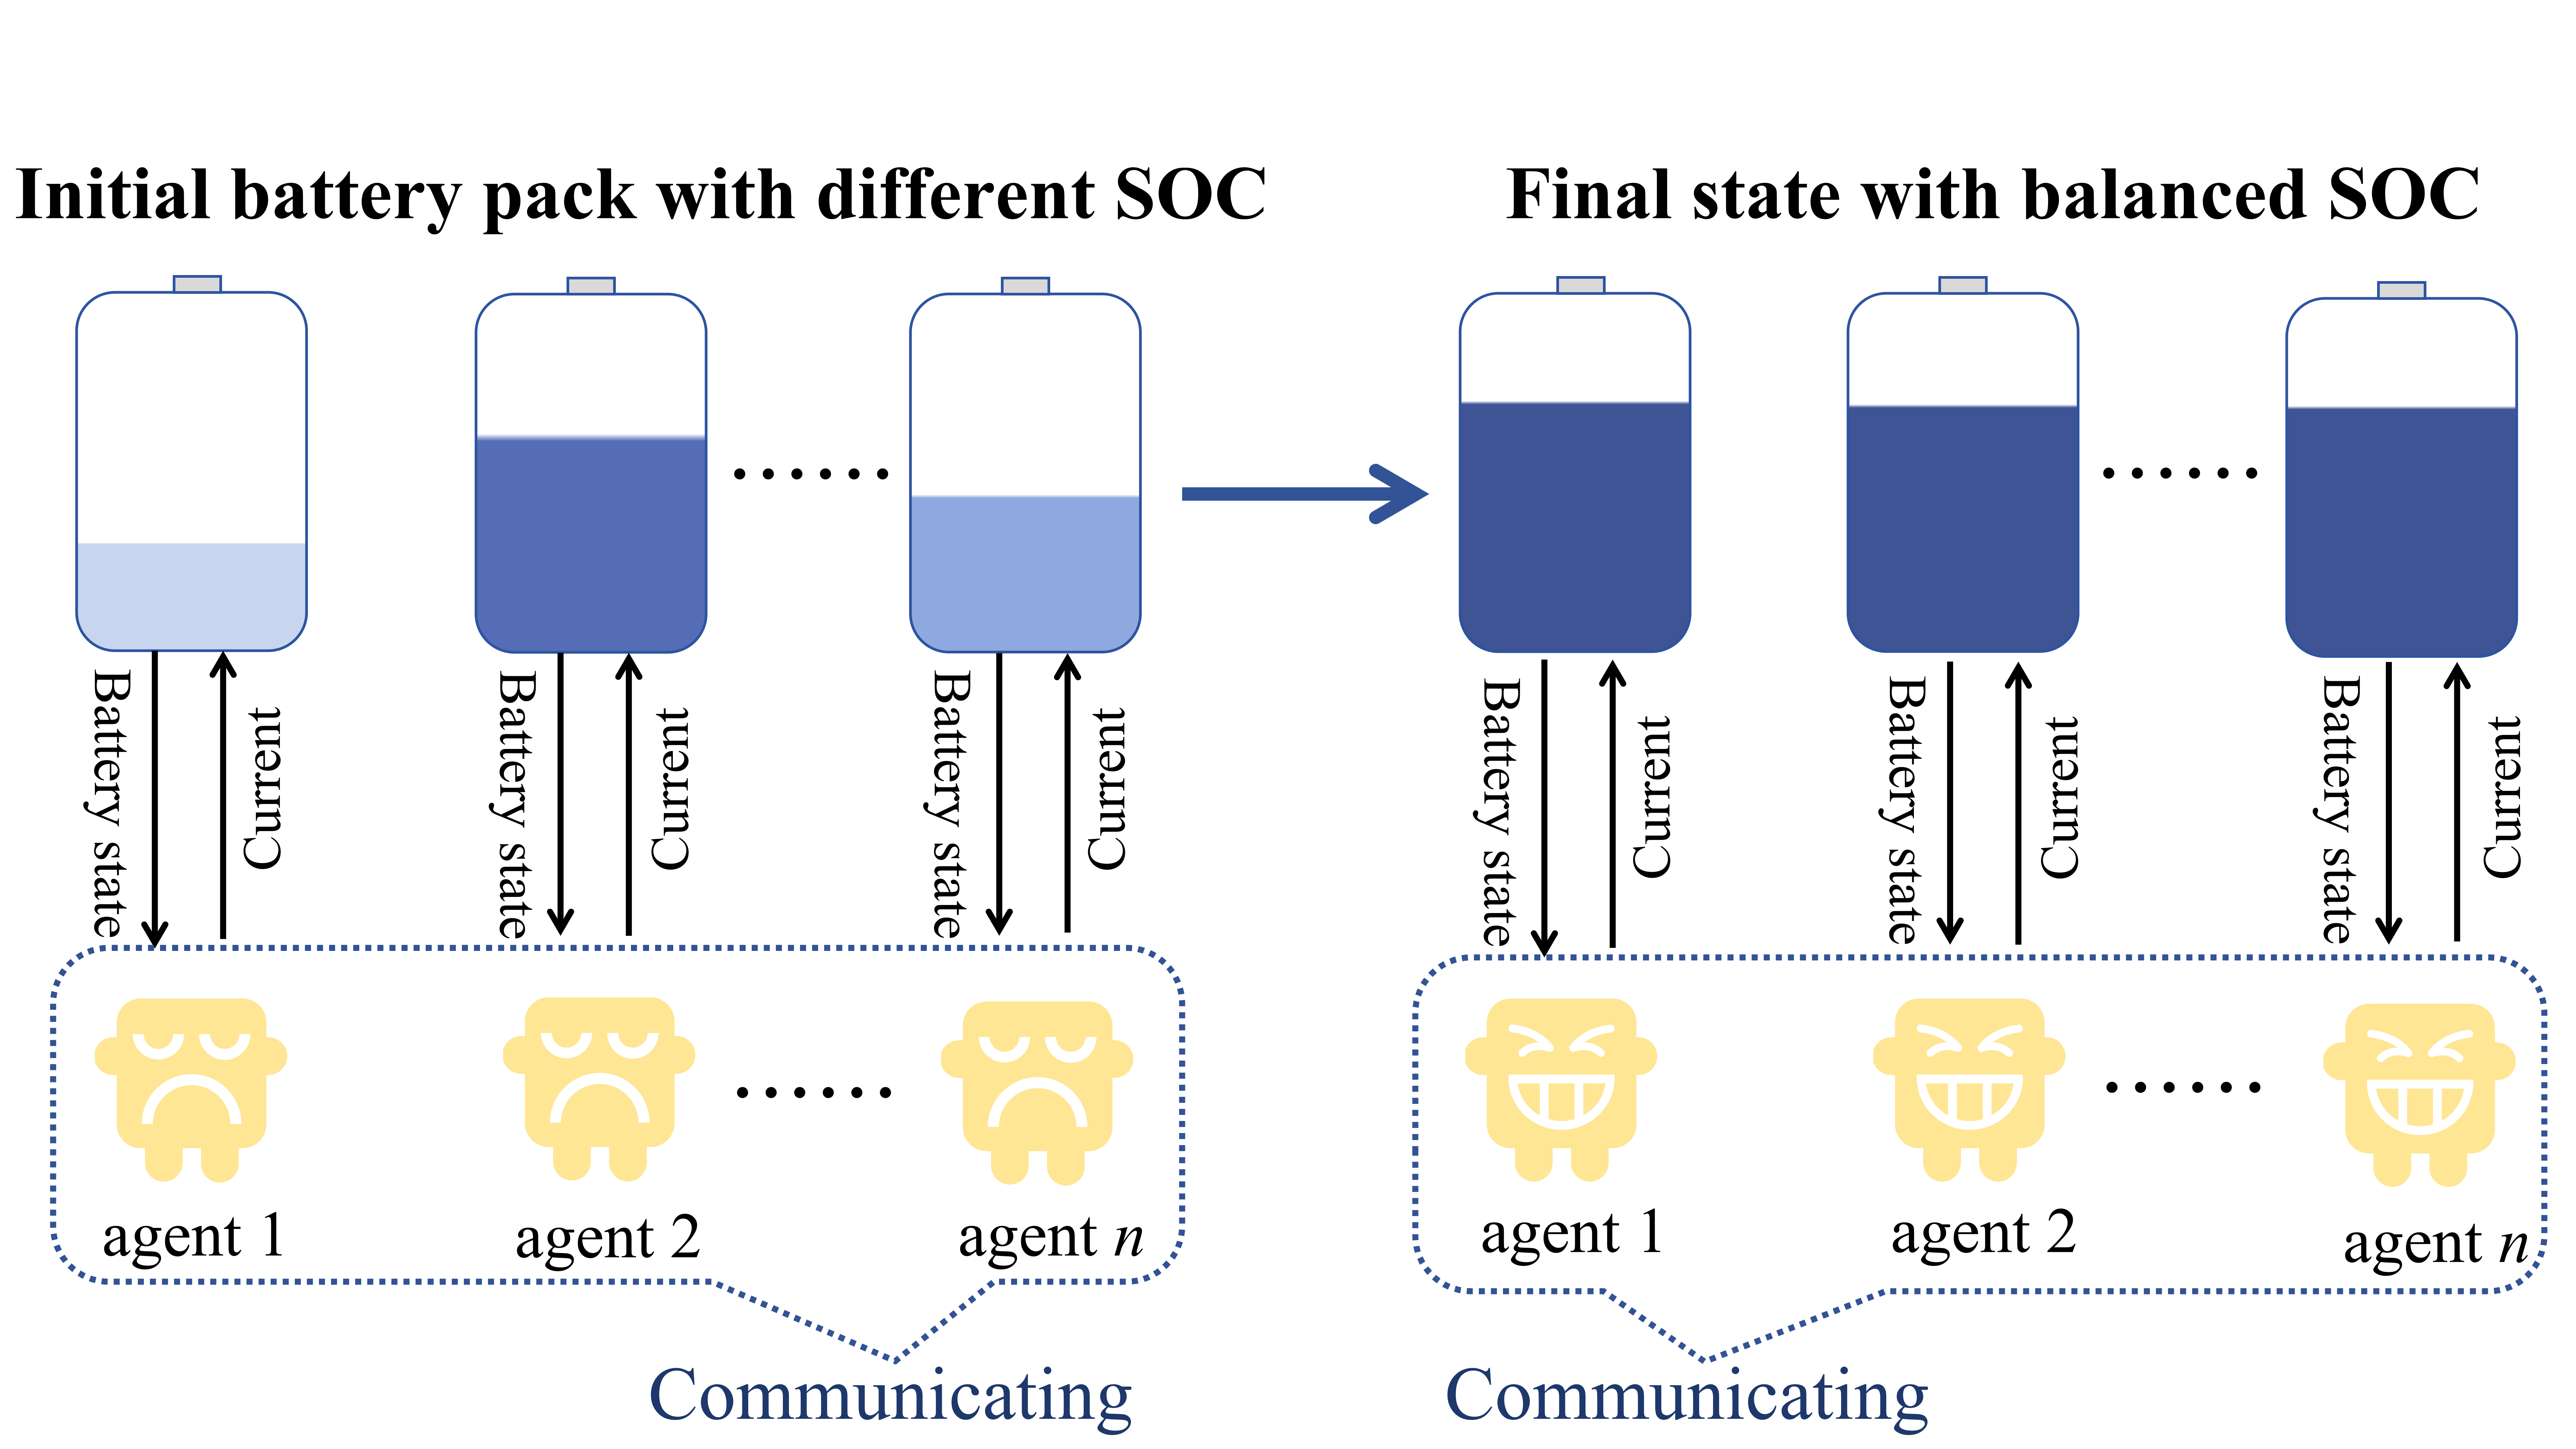
\includegraphics[width=1\linewidth]{image/figure1(2).png}
    \caption{Schematic of using the MARL-based framework to solve the charging balancing control problem.}
     \label{fig:MARL_Schematic}
 \end{figure}

\textbf{\begin{figure*}
    \centering
    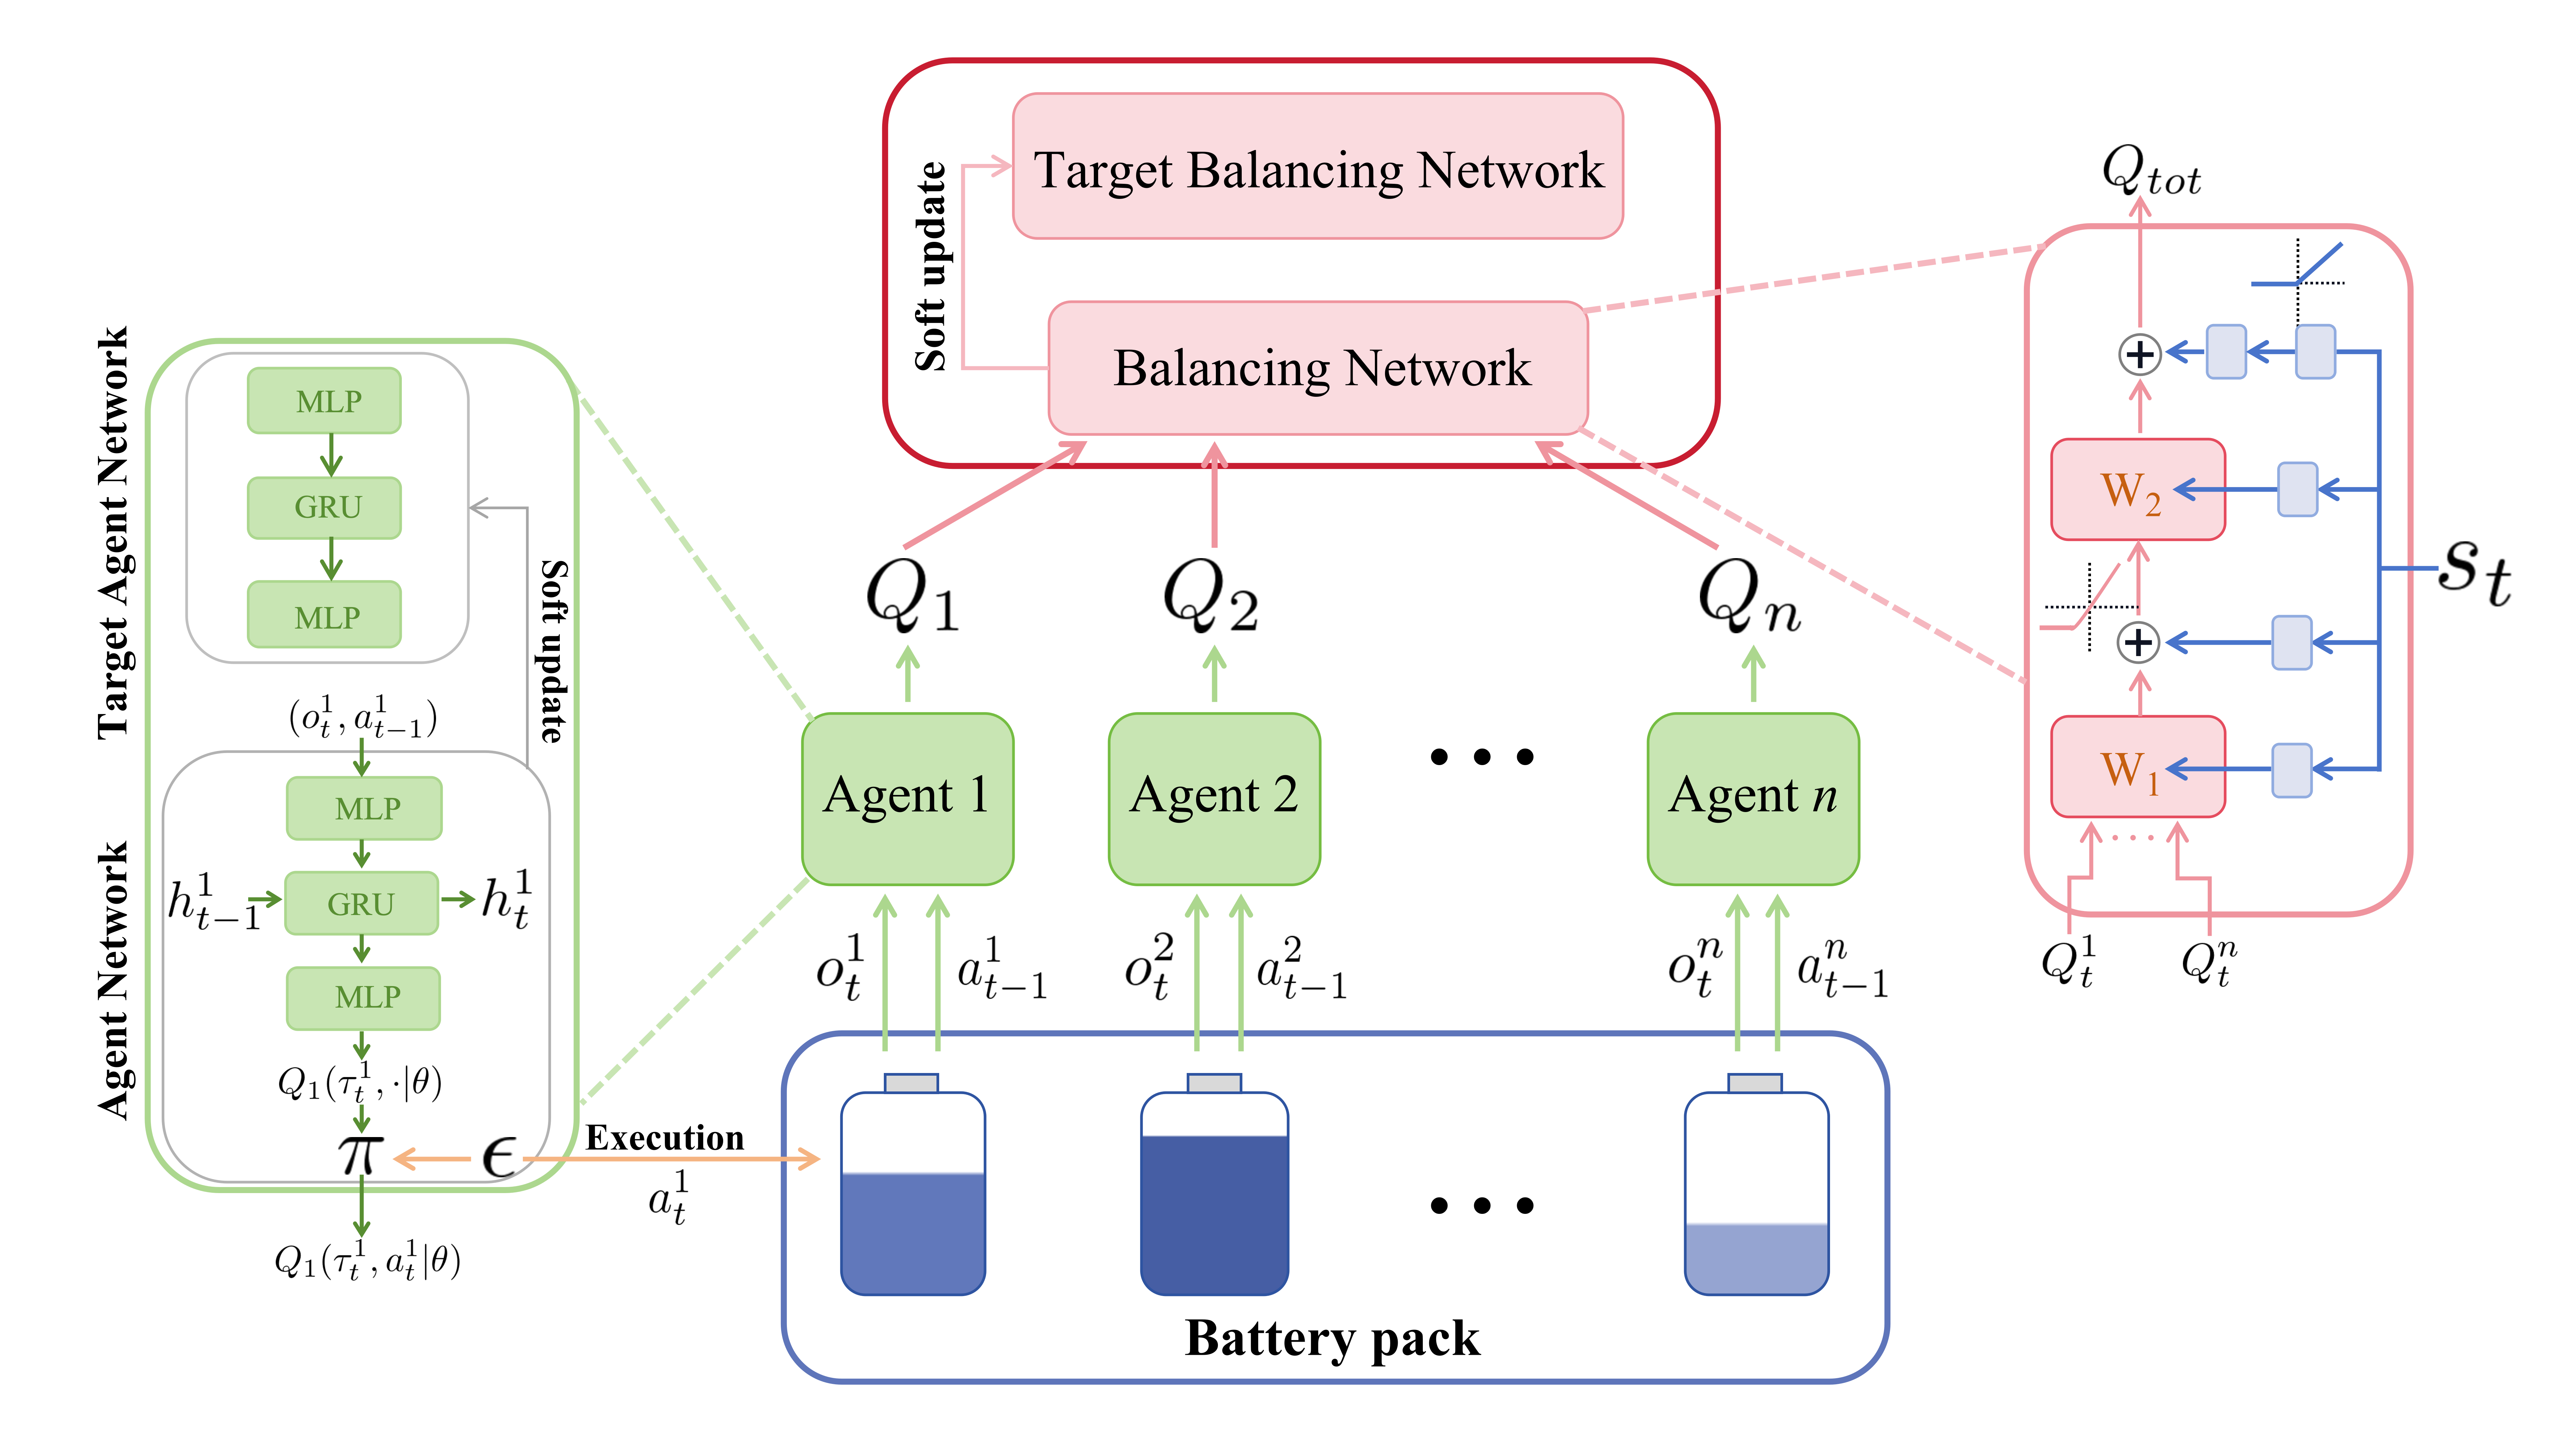
\includegraphics[width=0.9\textwidth,height=\textheight,keepaspectratio]{image/figure2.png}
    \caption{Schematic of the MBA-RL charging control framework. The left diagram depicts an agent network structure, which includes two multilayer perceptrons (MLP) and a gated recurrent unit (GRU). $\theta$ represents the parameters of the agent network. The right diagram illustrates the balancing network structure, where the hypernetworks (in blue) generate the weights and biases for the layers of the balancing network (shown in red), and $W_1$ and $W_2$  represent the two MLP layers.}
    \label{fig:schematic_method}
\end{figure*}}


\section{Proposed MBA-RL for Charging Balancing Control}
As shown in Fig. \ref{fig:MARL_Schematic}, in the conventional MARL-based framework, each agent independently defines a dedicated charging protocol for its respective cell while communicating with other agents to achieve SOC balancing across the entire battery pack. Consequently, each agent’s behavior is influenced not only by the environment but also by the actions of other agents, leading to a continuous evolution of each agent’s strategy. This creates a dynamically changing environment, making convergence in MARL particularly challenging. Additionally, gradient-based methods, such as the multi-agent deep deterministic policy gradient, struggle to quantify each agent’s contribution, hindering the effective capture of cooperative behavior.

To address this, we adopt QMIX as the MARL algorithm \cite{26} and integrate it with multiple SPMs as the environment to establish the charging control framework. The framework is capable of simultaneously implementing balancing control for multiple batteries and enabling fast charging for individual batteries. Afterward, we first present the MBA-RL charging control framework, followed by a detailed explanation of the MBA-RL design.


\subsection{MBA-RL Charging Control Framework}
The schematic of MBA-RL is presented in Fig.~\ref{fig:schematic_method}. As illustrated in Fig.~\ref{fig:schematic_method}, MBA-RL utilizes an architecture comprising agent networks, a balancing network, and a set of hyper-networks. For the $i$-th agent, the agent network is modeled as a deep recurrent Q-network, which integrates the current observation $o_t^i$ at each time step with the previous action $a_{t-1}^i$ to form the action-observation history $\tau_t^i$ and generate the corresponding $Q_i$. The balancing network is a feed-forward neural network, which integrates the local Q-values of individual agents (i.e., $Q_1, Q_2, \dots, Q_n$) into the framework's joint Q-value $Q_{\text{tot}}$, based on each agent’s contribution to the global objective. The hyper-networks generate the weights for the balancing network. Furthermore, we employ multiple target agent networks and a target balancing network to reduce environmental fluctuations and mitigate volatility in the estimation of the Q-value function.


% In MBA-RL, the $i$-th agent relies on local observation $o_t^i$ and action $a_t^i$ at the time step $t$, and adjusts strategies based on individual action-observation histories $\tau_t^i = \left[o_1^i, a_1^i, ..., o_t^i, a_t^i\right]^{\mathrm{T}}$ to generate $Q_i$. Additionally, MBA-RL integrates the local Q-values of individual agents (i.e., $Q_1, Q_2, \dots, Q_n$) into the framework's joint Q-value $Q_{\text{tot}}$ through the balancing network, based on each agent’s contribution to the global objective. This allows agents to accurately evaluate the impact of their actions and refine their policies accordingly, fostering an effective balance-aware control strategy. Moreover, we employ multiple target agent networks and a target balancing network to reduce environmental fluctuations and mitigate volatility in the estimation of the Q-value function.

To further elaborate on how MBA-RL addresses the charging balancing control problem, we first formulate \eqref{eqn:balancing objective} as a Dec-POMDP \cite{27} described by a tuple \(T = \langle\mathcal{S}, \mathcal{A}, \mathcal{R}, \mathcal{S'}, \mathcal{P}, done\rangle\). Each component of this tuple is outlined in detail below.

\subsubsection{State Space} The state space $\mathcal{S}$ encompasses all possible states of the battery pack, $\mathbf{s}_t \in \mathcal{S}$ is formed by the combination of the observations from all agents at the time step $t$:
\begin{equation}
   \mathbf{s}_t = \left[ o_t^1, o_t^2, \dots, o_t^n \right]^{\mathrm{T}}
\end{equation}
where the $i$-th agent’s observation $o_t^i$ consists of three components: the battery voltage (denoted as $V_i(t)$), average temperature (denoted as $T_i(t)$), and SOC (denoted as $SOC_i(t)$).

\subsubsection{Action Space} The action space $\mathcal{A}$ consists of the charging currents output by all agents. At the time step $t$, each agent chooses an action $a_t^i$ (i.e., $I_i(t)$), collectively forming a joint action $\mathbf{a}_t \in \mathcal{A}$:
\begin{equation}
\mathbf{a}_t = \left[ a_t^1, a_t^2, \dots, a_t^n \right]^{\mathrm{T}}.
\end{equation}
\subsubsection{Reward Function} The reward function $\mathcal{R}$ can be determined based on the objective and the safety constraints, and $r_t \in \mathcal{R}$ represents the total environmental reward at the time step $t$ after all agents have executed their actions:
\begin{equation}
    r_t = r_{\text{time}} + r_{\text{bal}} + r_{\text{safety}}
\end{equation}
where $r_{\text{time}} \stackrel{\Delta}{=} -0.75$ denotes the penalty applied at each time step before the termination condition is reached, designed to accelerate the charging process.

Then $r_{\text{bal}}$ can be calculated as follows:
\begin{equation}
  r_{\text{bal}} = 
\begin{cases}
-50(\sigma - \beta), & \text{if } \sigma \geq \beta \\
0, & \text{otherwise}
\end{cases}  
\end{equation}
where $\sigma$ denotes the standard deviation of the SOC across all cells in the battery pack, $\beta$ indicates the predefined threshold, and $r_{\text{bal}}$ characterizes the imbalance effects in the battery pack. 

As shown in \eqref{safty condition}, $r_{\text{safety}}$ is divided into voltage safety constraints and temperature safety constraints:
\begin{equation}
    r_{\text{safety}} = r_{\text{volt}} + r_{\text{temp}}
\end{equation}
\begin{equation}
    \quad r_{\text{volt}} = \sum_{i=1}^{n} \delta_{v,i}, \quad r_{\text{temp}} = \sum_{i=1}^{n} \delta_{t,i}
\end{equation}
% \begin{equation}
%     r_{\text{temp}} = \sum_{i=1}^{n} \delta_{t,i}
% \end{equation}
where $\delta_{v,i}$ and $\delta_{t,i}$ represent the overvoltage and overtemperature penalties of the $i$-th cell, respectively:
\begin{equation}
    \delta_{v,i} = 
\begin{cases}
-20(V_i(t) - V_{\text{max}}), & \text{if } V_i(t) \geq V_{\text{max}} \\
0, & \text{otherwise}
\end{cases}
\end{equation}

\begin{equation}
  \delta_{t,i} = 
\begin{cases}
-2(T_i(t) - T_{\text{max}}), & \text{if } T_i(t) \geq T_{\text{max}} \\
0, & \text{otherwise}
\end{cases}  .
\end{equation}
\subsubsection{Others} $\mathbf{s}_{t+1} \in \mathcal{S'}$ is the states at the next time step of the battery pack after taking $\mathbf{a}_t$. $\mathcal{P}(\mathbf{s}_{t+1}|\mathbf{s}_t, \mathbf{a}_t)$ is the state transition function, representing the probability of transitioning from $\mathbf{s}_t$ to $\mathbf{s}_{t+1}$ given the joint action $\mathbf{a}_t$. $done$ denotes the indicator for the completion of the balancing process.

\begin{algorithm}[t]
    \caption{MBA-RL charging control framework}
    \label{alg:QMIX}
    
    \begin{algorithmic}[1]
        \STATE Initialize $\theta, \theta', \bm{\theta}, \bm{\theta}'$ randomly
        \STATE Set the learning rate $\alpha$, number of episodes $N_{episode}$, and replay buffer $\mathcal{D}$
        \STATE $\theta' \leftarrow \theta, \bm{\theta}' \leftarrow \bm{\theta}$
        \FOR{$episode =$ 1 to $N_{episode}$}
            \STATE $t\leftarrow 0$, $\tau_t^i \leftarrow \emptyset$, and observe the initial state $\mathbf{s}_t$

            // \textbf{Data Collection}
            \WHILE{$\neg done$}
                \FOR{the $i$-th agent}
                    \STATE $\tau_t^i \leftarrow \tau_{t-1}^i \cup \{(o_t^i, a_{t-1}^i)\}$
                    \STATE $\epsilon \gets 0.5 (1 - \frac{episode}{N_{episode}})$
                    \STATE Select $a_t^i$ according to \eqref{epsilon-greedy}
                \ENDFOR
                \STATE Execute the joint action $\mathbf{a}_t$, observe the reward $r_t$, and get the next state $\mathbf{s}_{t+1}$
                \STATE $\mathcal{D} \leftarrow \mathcal{D} \cup \{ \langle\mathbf{s}_t, \mathbf{a}_t, r_t, \mathbf{s}_{t+1}, done\rangle \}$
            \ENDWHILE
            
            // \textbf{Network Update}
            \IF{$|\mathcal{D}| > N$}
                \STATE $B \leftarrow$ Randomly sample data from $N$ episodes in $\mathcal{D}$
                \FOR{each time step $t$ in each episode in batch $B$}
                    \STATE Calculate $Q_{tot}$ by \eqref{Q-value} based on the state $\mathbf{s}_t$
                    \STATE Calculate $y^{\text{tot}}$ by \eqref{target Q} based on the state $\mathbf{s}_{t+1}$
                \ENDFOR
                \STATE Under the conditions given in \eqref{QMIX_constraints} and \eqref{QMIX_constraints_1}, utilize the RMSprop  optimizer \cite{zou2019sufficient} to update $\theta$ and $\bm{\theta}$ by minimizing the loss function: $\left( y_{\text{tot}} - Q_{\text{tot}} \right)^2$
            \ENDIF
            \IF{$episode$ \% $N_t$ == 0}
                \STATE $\theta' \leftarrow \theta$, $\bm{\theta}' \leftarrow \bm{\theta}$ 
            \ENDIF
        \ENDFOR
    \end{algorithmic}
\end{algorithm}

\subsection{Balancing Mechanism of MBA-RL}

\begin{figure}[t]
    \centering
    \includegraphics[width=0.95\linewidth]{image/experiment platform.png}
    \caption{Schematic of the experimental platform.}
    \label{fig:experiment_Schematic}
\end{figure}

The core of MBA-RL lies in leveraging global information to enhance the decision-making process of each agent. This enables agents to consider the overall balancing objective defined in \eqref{eqn:balancing objective} while maximizing individual performance, thereby fostering collaboration among different agents. 

In MBA-RL, the $i$-th agent aims to optimize its local Q-value, denoted as $Q_i(\tau_t^i, a_t^i|\theta)$, to maximize the global Q-value $Q_{\text{tot}}$. This involves balancing the agent's own goals of safety and fast charging while simultaneously contributing to the rapid achievement of balance within the battery pack. Each agent chooses its current action $a_t^i$ using the $\epsilon$-greedy strategy, which can be described as follows:
\begin{equation}\label{epsilon-greedy}
a_t^i =
\begin{cases}
\text{random available action} & \text{with probability } \epsilon \\
\arg\max_{a_t^i} Q_i(\tau_t^i, a_t^i|\theta) & \text{with probability } 1 - \epsilon
\end{cases}
\end{equation}
where $Q_i(\tau_t^i, a_t^i|\theta)$ is computed based on $\tau_t^i$ and $a_t^i$. Note that all agents employ a unified set of parameters $\theta$ to improve MBA-RL’s generalization capability and efficiency.

The balancing network takes the outputs of all agent networks as inputs and combines them in a monotonic fashion to generate the values of $Q_{tot}(\boldsymbol{\tau}_t, \mathbf{a}_t|\bm{\theta})$:
\begin{equation}\label{Q-value}
    Q_{tot}(\boldsymbol{\tau}_t, \mathbf{a}_t|\bm{\theta}) = f(Q_1(\tau_t^1, a_t^1|\theta), ..., Q_n(\tau_t^n, a_t^n|\theta))
\end{equation}
where $\boldsymbol{\tau}_t$ denotes the joint action-observation history at the time step $t$, and $\bm{\theta}$ represents the parameters of the balancing network. 

The final objective of MBA-RL is to maximize the global Q-value $Q_{tot}(\boldsymbol{\tau}_t, \mathbf{a}_t|\bm{\theta})$. The balancing network achieves this by enforcing a monotonicity constraint between the global Q-value and each agent’s Q-value. This constraint guarantees that maximizing each agent’s Q-value leads to the maximization of the global Q-value:
\begin{equation}\label{QMIX_constraints}
\arg\max_{\mathbf{a}_t} Q_{tot}(\boldsymbol{\tau}_t, \mathbf{a}_t|\bm{\theta}) =
\begin{pmatrix}
\arg\max_{a_t^1} Q_1(\tau_t^1, a_t^1|\theta) \\
\vdots \\
\arg\max_{a_t^n} Q_n(\tau_t^n, a_t^n|\theta)
\end{pmatrix}.
\end{equation}
Eq. \eqref{QMIX_constraints} enables each agent to greedily select the action that maximizes $Q_i(\tau_t^i, a_t^i|\theta)$ for decentralized execution. 

Next, the weights of the balancing network are generated by different hyper-networks. Each hyper-network receives the state $s_t$ as input and outputs the weights for a specific layer of the balancing network. To guarantee \eqref{QMIX_constraints}, the weights of the balancing network are strictly constrained to be non-negative:
\begin{equation}\label{QMIX_constraints_1}
\frac{\partial Q_{tot}}{\partial Q_i} \geq 0, \, i = 1, 2, ..., n.
\end{equation}

The initial parameters of the multiple target agent networks (denoted as $Q_i(\tau_t^i, a_t^i|\theta'), i = 1, ..., n$) and the target balancing network (denoted as $Q_{tot}(\boldsymbol{\tau}_t, \mathbf{a}_t|\bm{\theta}')$) are directly copied from  $\theta$  and  $\bm{\theta}$, respectively. Moreover, $\theta'$  and  $\bm{\theta}'$ are updated less frequently, with updates occurring every $N_t$ episodes. The global target Q-value can be computed using target networks:
\begin{equation}\label{target Q}
y^{\text{tot}} = r_t + \gamma \max_{\mathbf{a}_{t+1}} Q_{\text{tot}}(\boldsymbol{\tau}_{t+1}, \mathbf{a}_{t+1}|\bm{\theta}').
\end{equation}

Additionally, to obtain sufficient data for training MBA-RL, the experience tuple $\langle\mathbf{s}_t, \mathbf{a}_t, r_t, \mathbf{s}_{t+1}, done\rangle$ is stored in the replay buffer $\mathcal{D}$. During training, we randomly sample a batch of episodes to update the network parameters. The replay buffer effectively mitigates data correlation and enhances sampling efficiency. Moreover, employing batch updates stabilizes the training process and mitigates the risk of overfitting.

In summary, the details of the MBA-RL charging control framework are described in Algorithm 1, where $|\cdot|$ denotes the cardinality of a set.

\begin{figure}[t]
    \centering

    \begin{subfigure}[t]{0.24\textwidth} 
        \centering
        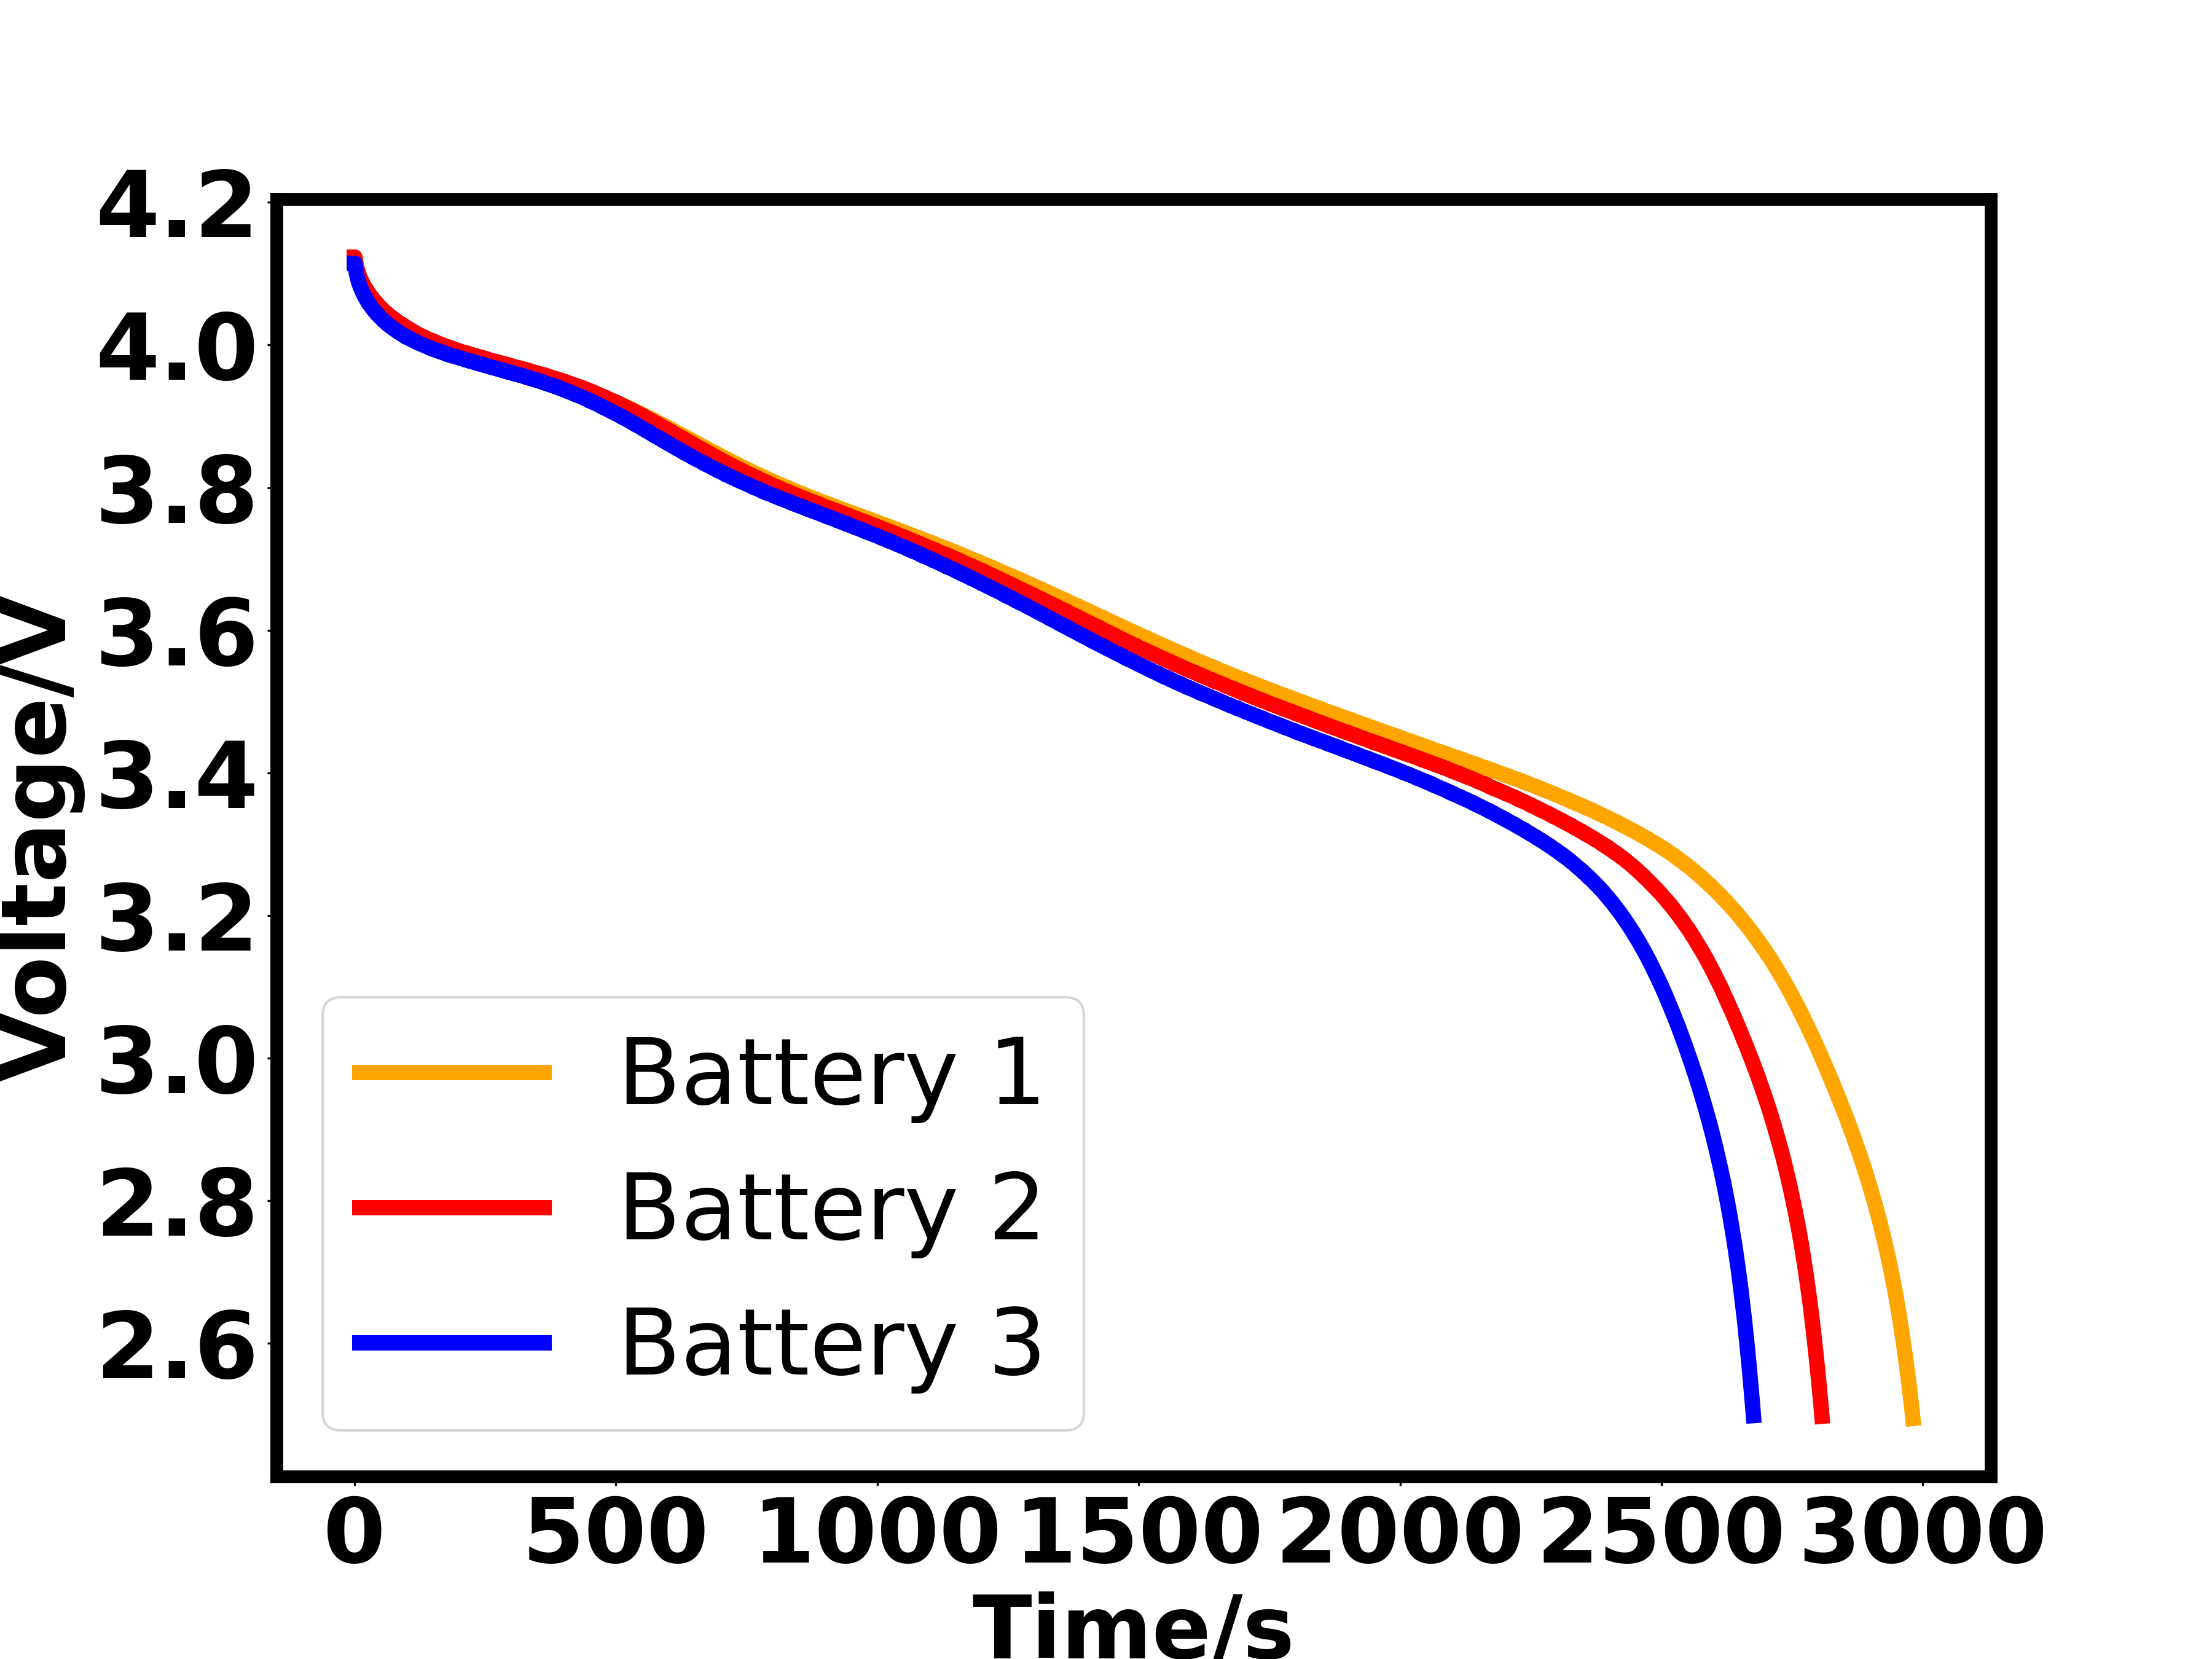
\includegraphics[width=\textwidth]{image/Voltage.png}
        \caption{}
    \end{subfigure}
    \hfill
    \begin{subfigure}[t]{0.24\textwidth}
        \centering
        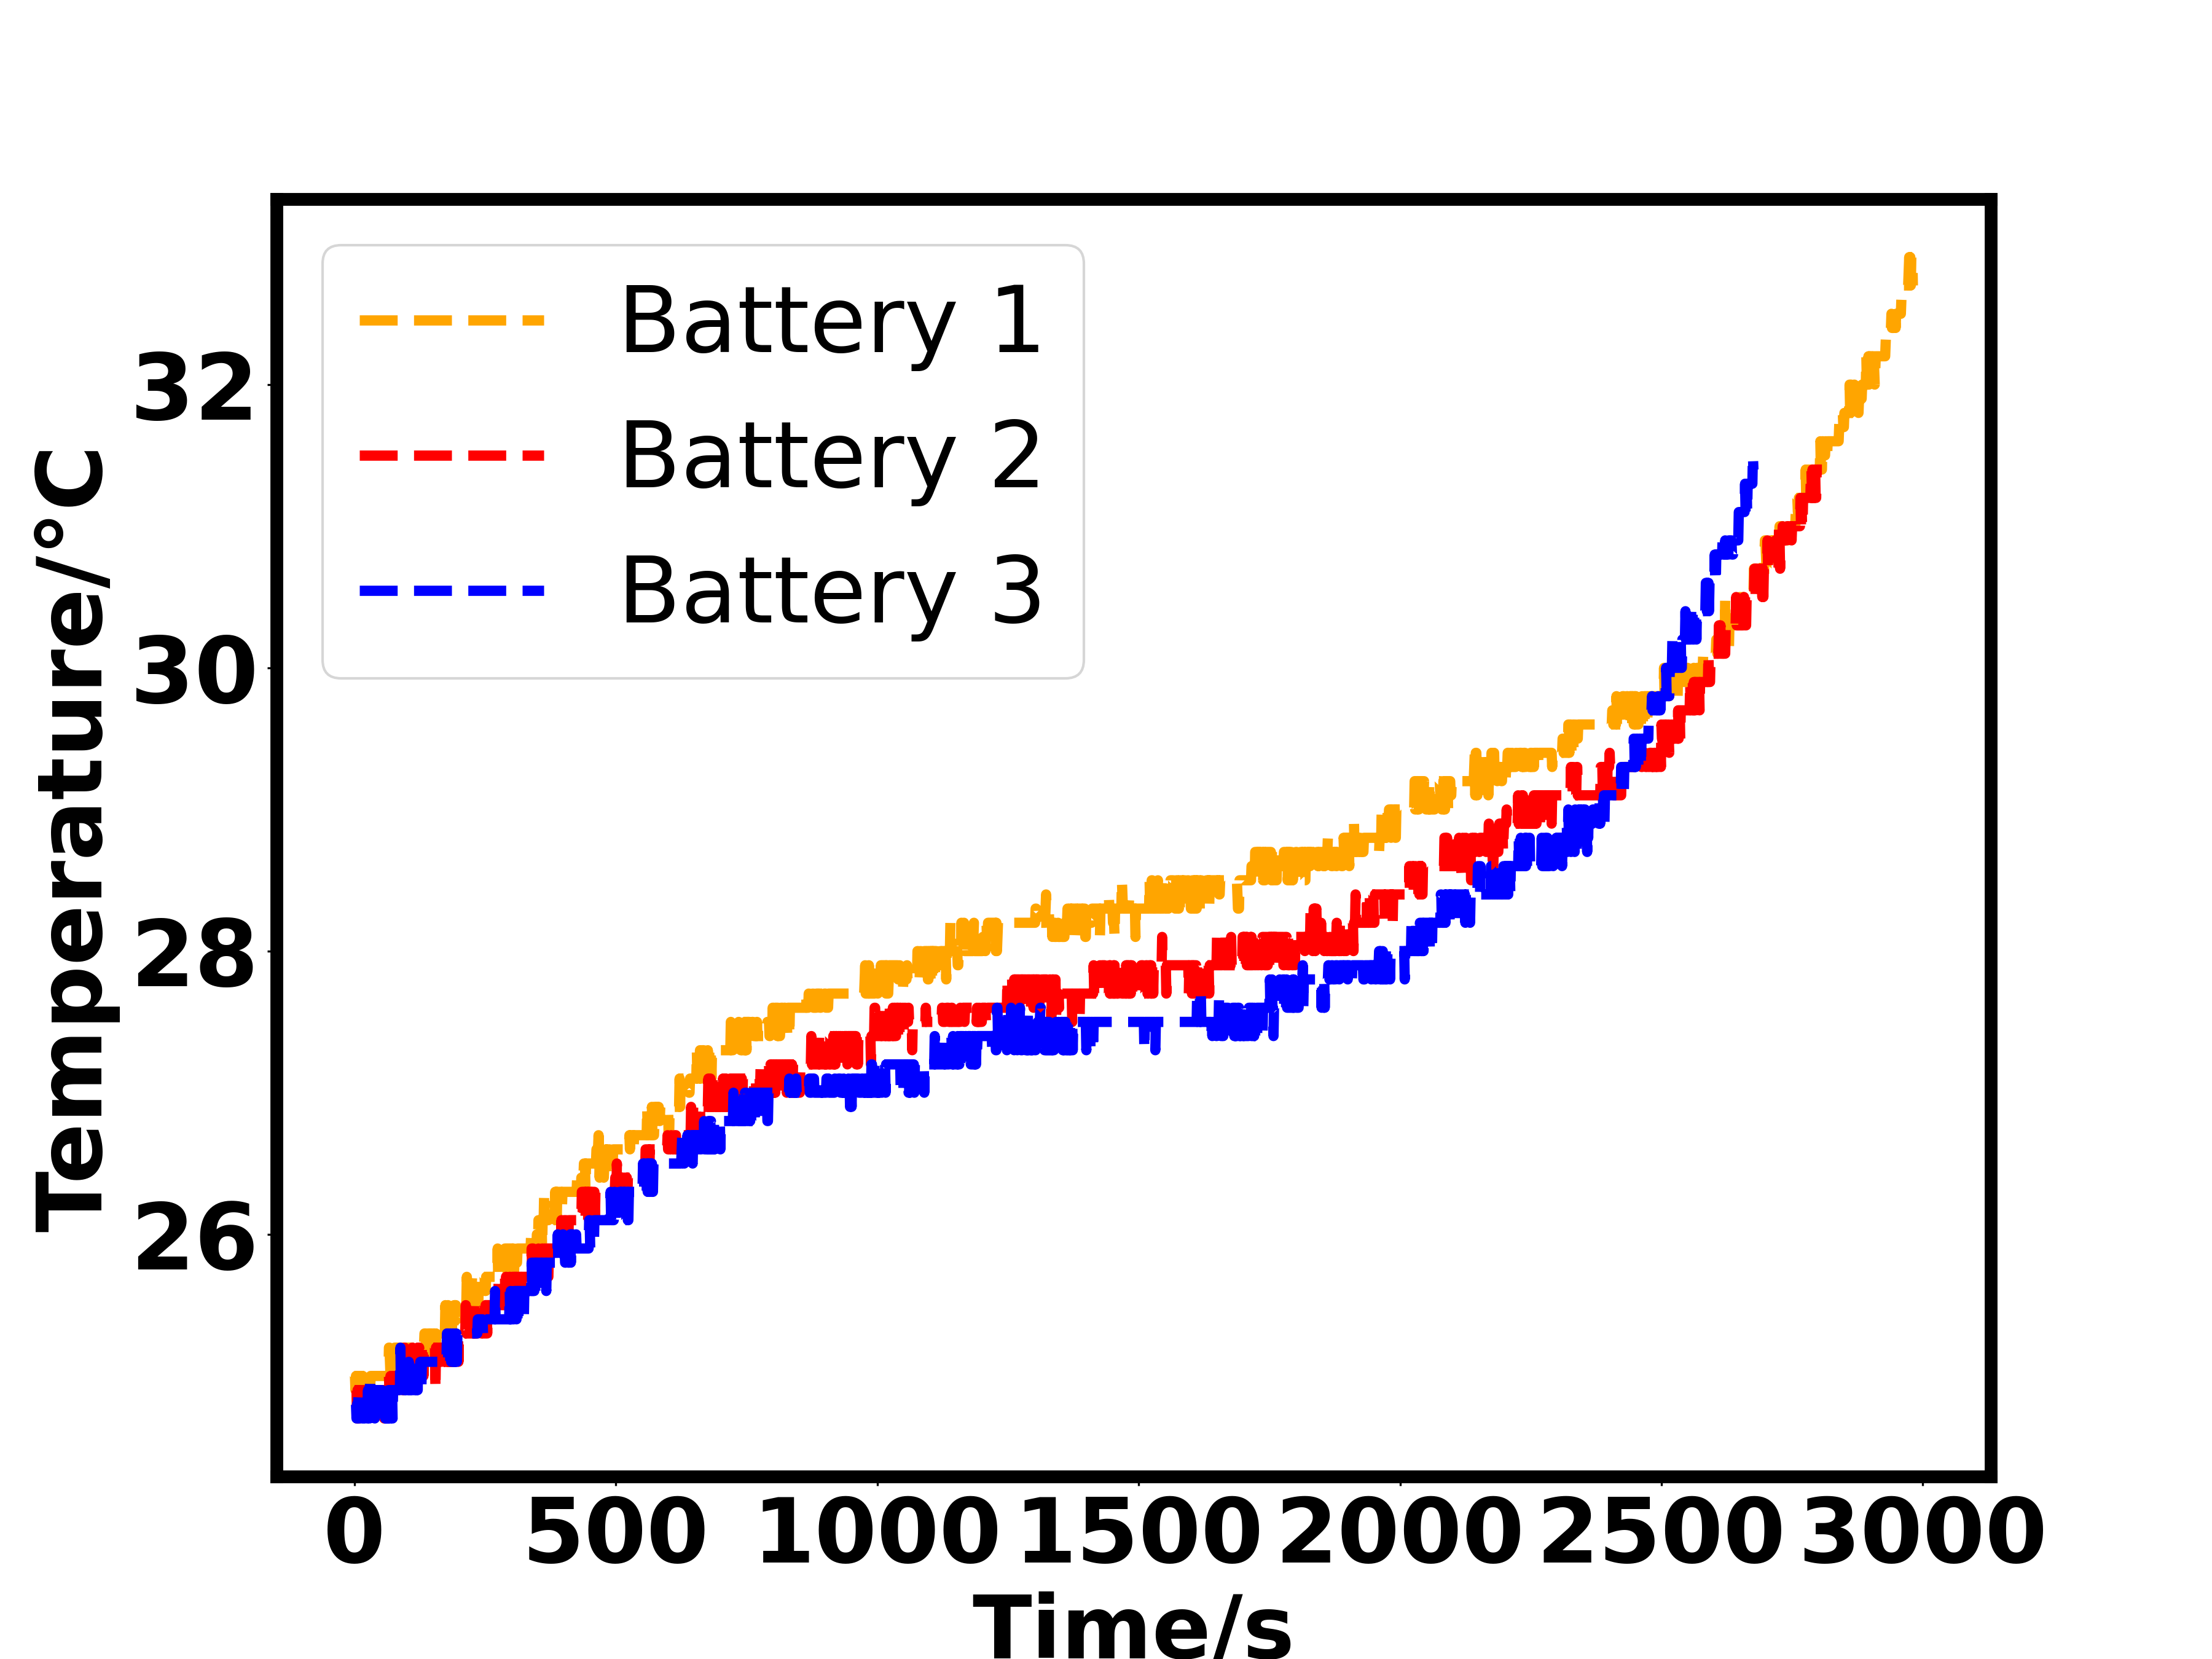
\includegraphics[width=\textwidth]{image/Temperature.png} 
        \caption{}
    \end{subfigure}

    \caption{Voltage and temperature curves of the three batteries at 1 C discharging current. (a) Voltage curve. (b) Temperature curve.}
    \label{fig:three_aging}
\end{figure}

\begin{figure}[t]
    \centering

    \begin{subfigure}[t]{0.24\textwidth} 
        \centering
        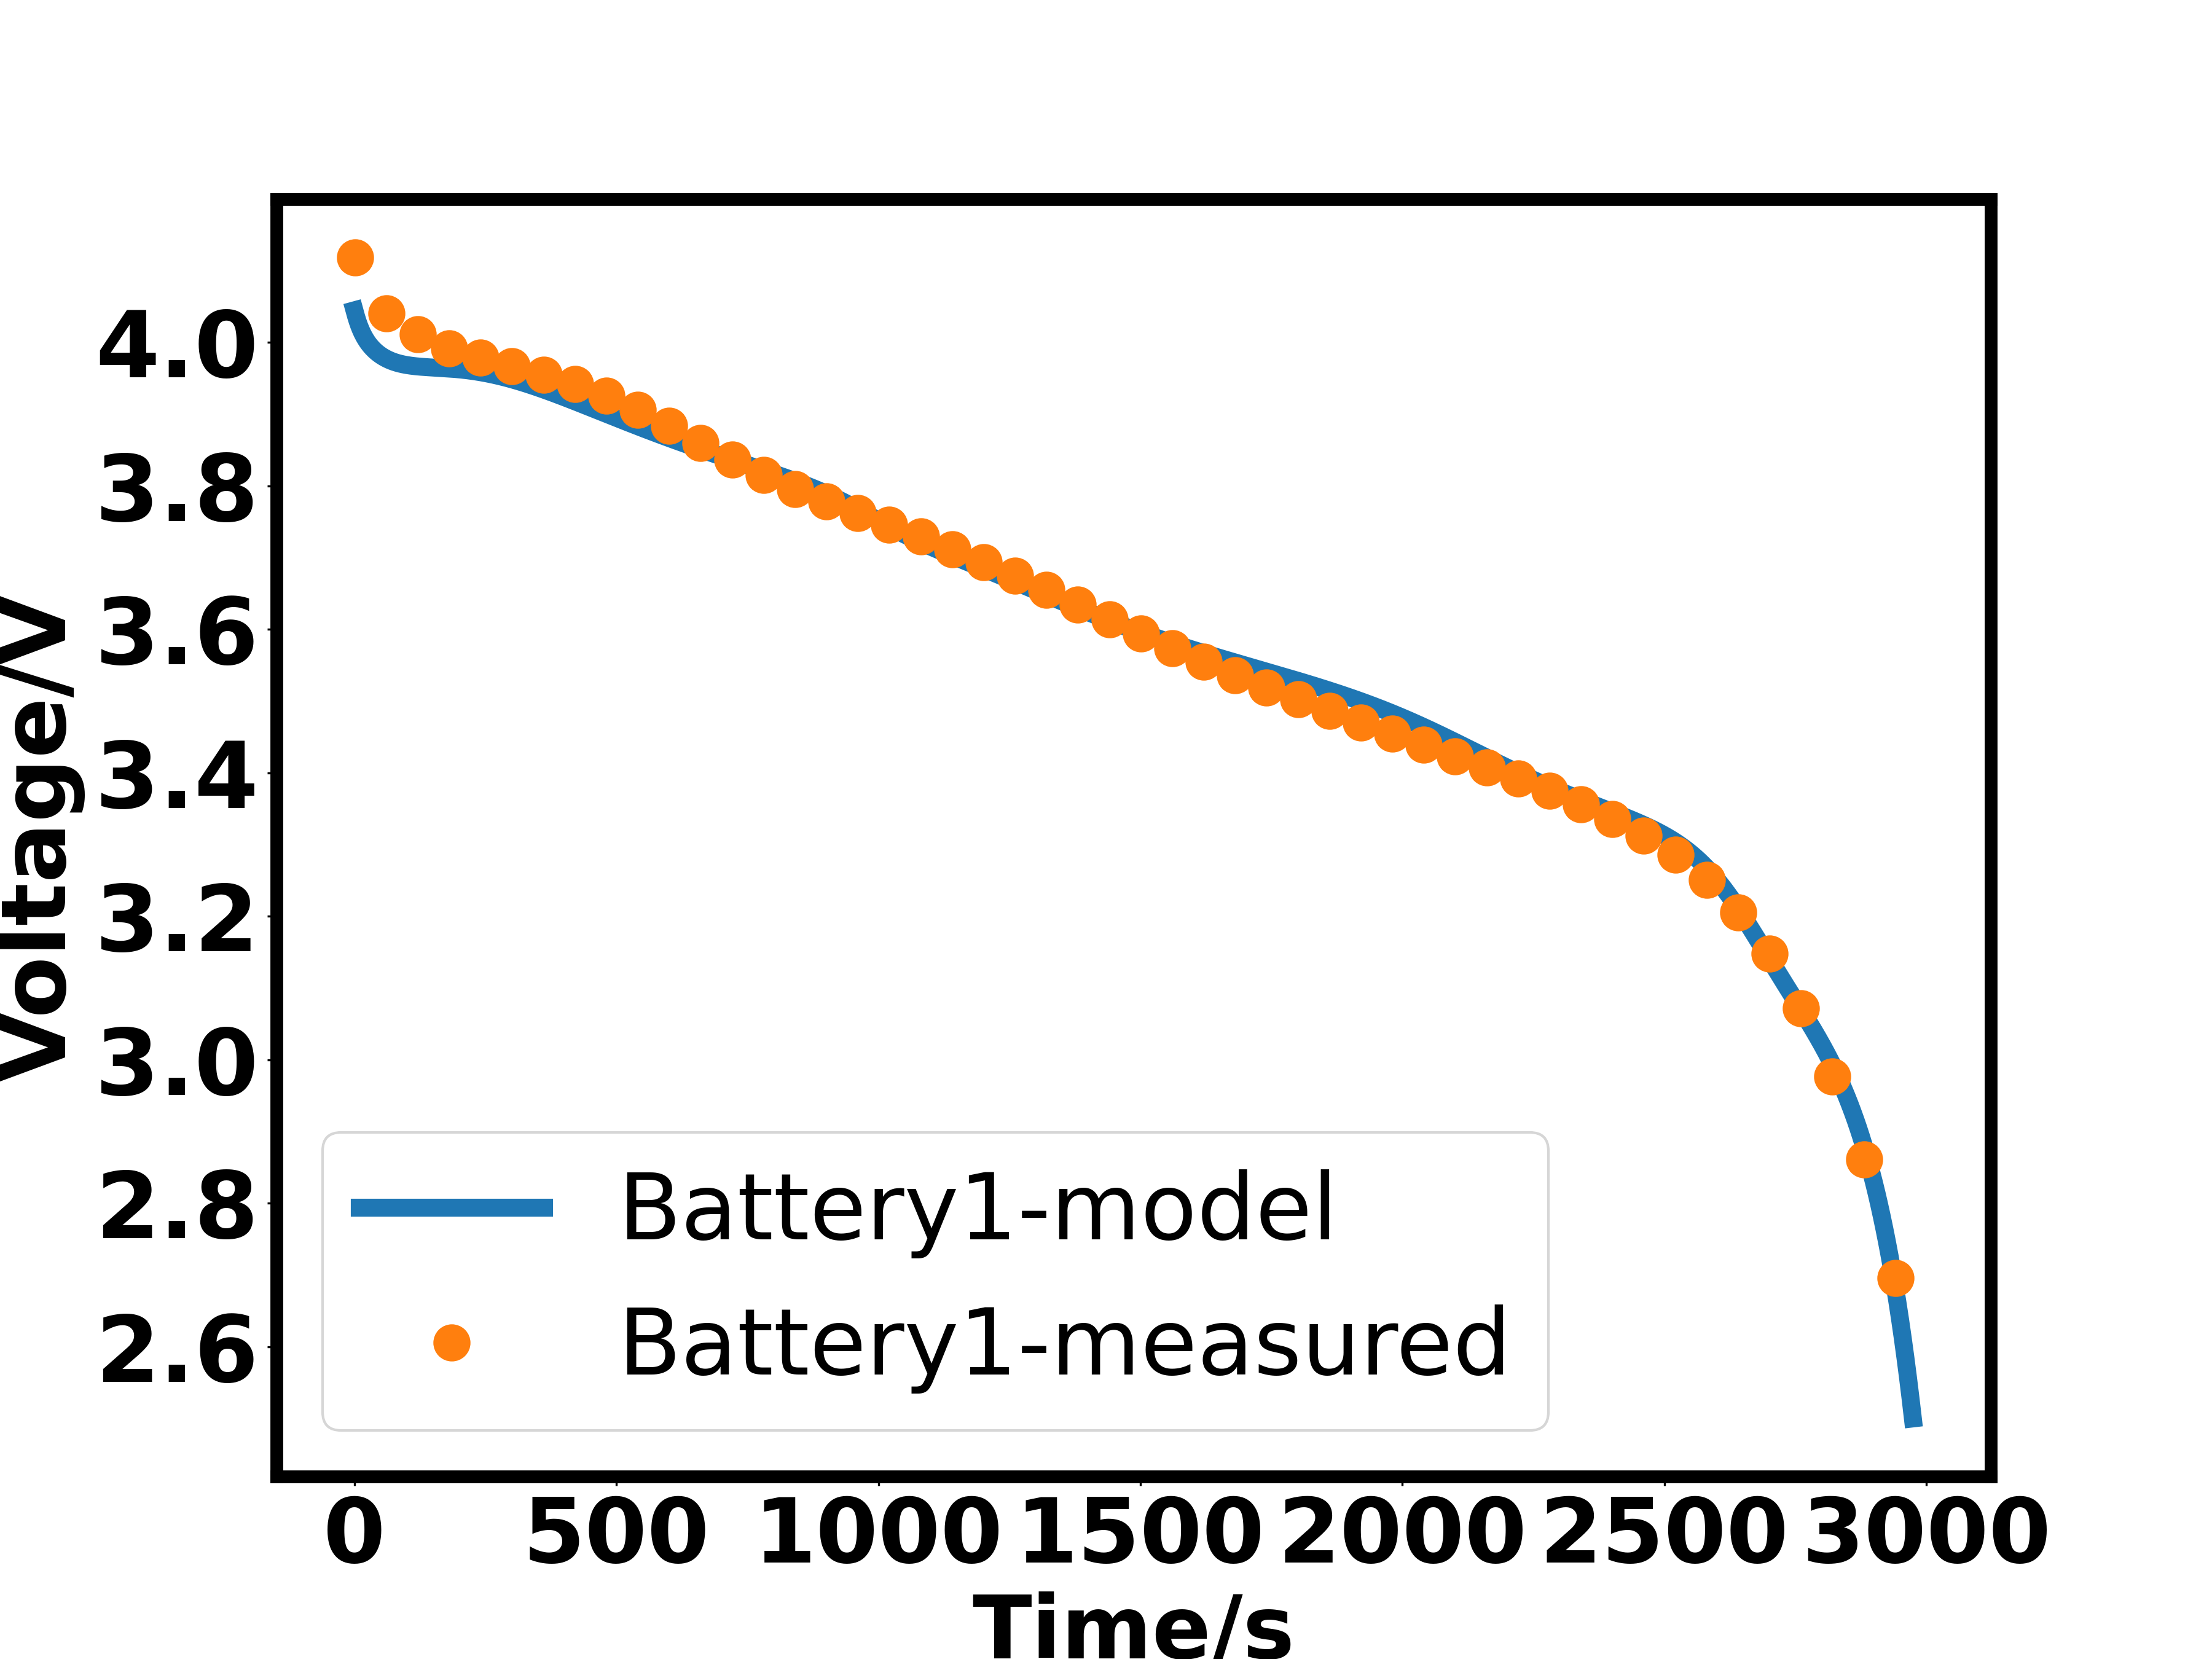
\includegraphics[width=\textwidth]{image/Battery1_volt.png}
        \caption{}
    \end{subfigure}
    \hfill
    \begin{subfigure}[t]{0.24\textwidth}
        \centering
        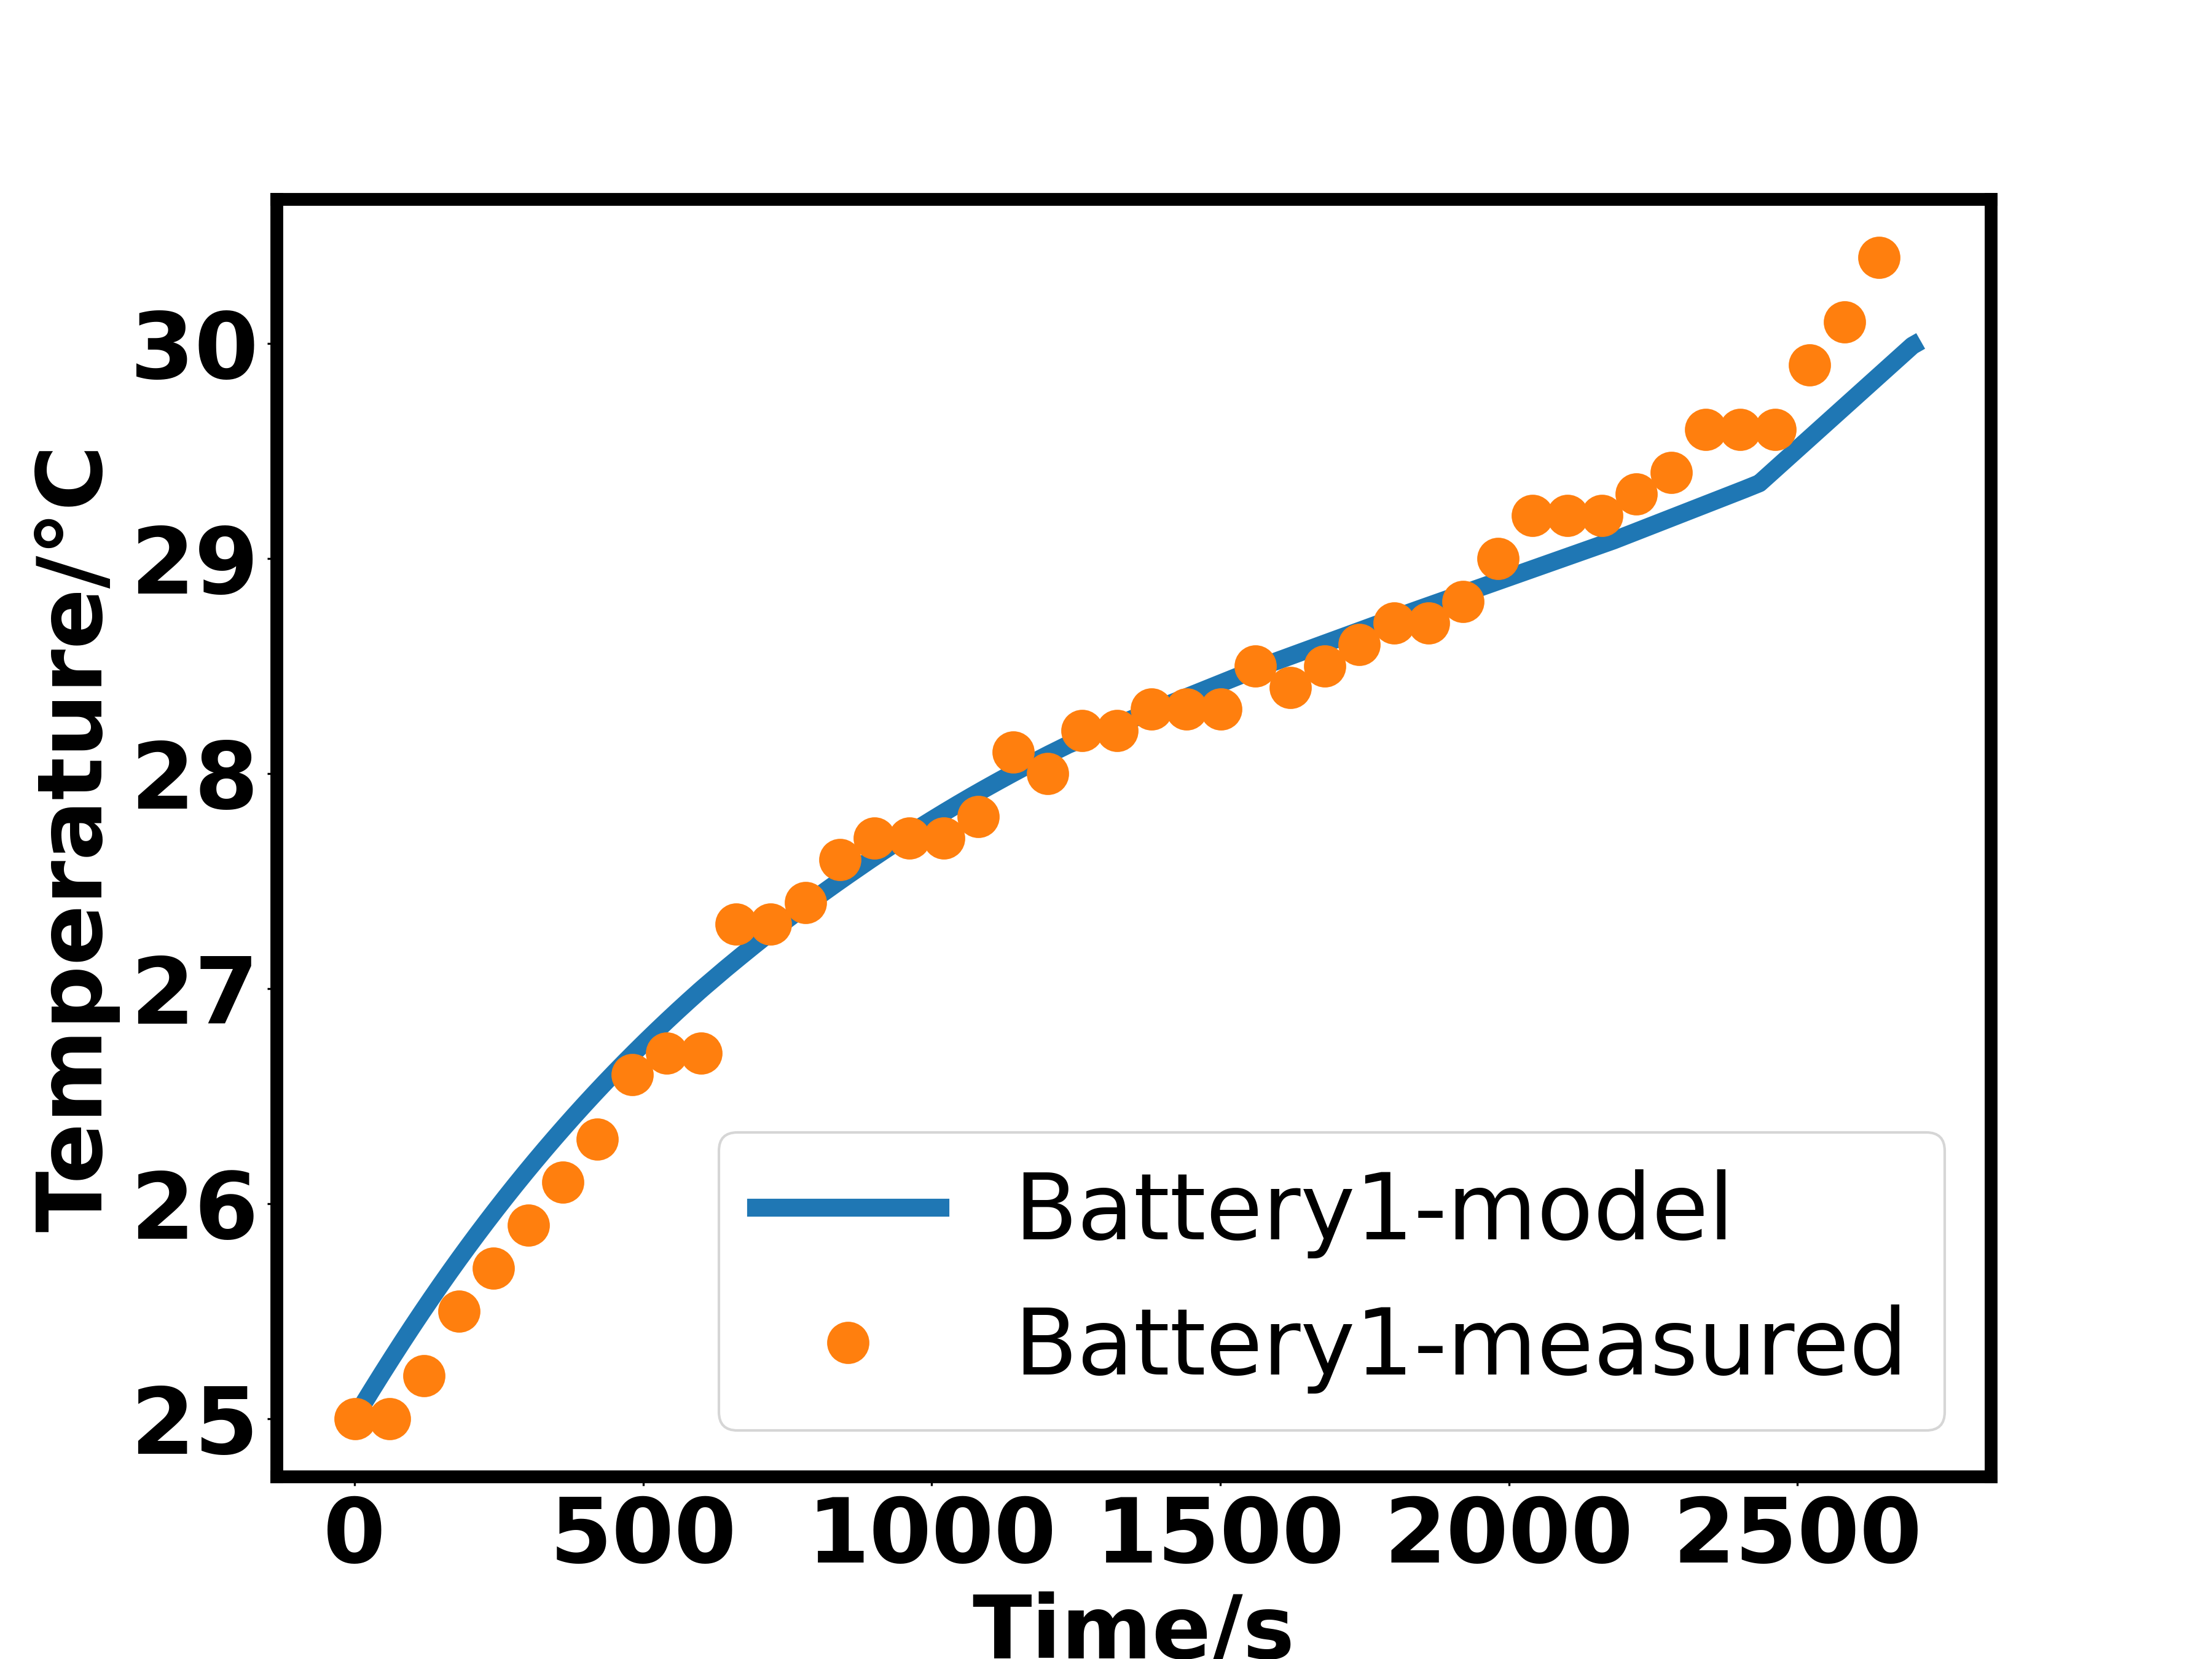
\includegraphics[width=\textwidth]{image/Battery1_temp.png} 
        \caption{}
    \end{subfigure}

    \caption{Parameter identification results for $Battery\;1$. (a) Electrochemical model parameter identification. (b) Thermal model parameter identification.}
    \label{battery1}
\end{figure}

\begin{figure}[t]
    \centering

    \begin{subfigure}[t]{0.24\textwidth} 
        \centering
        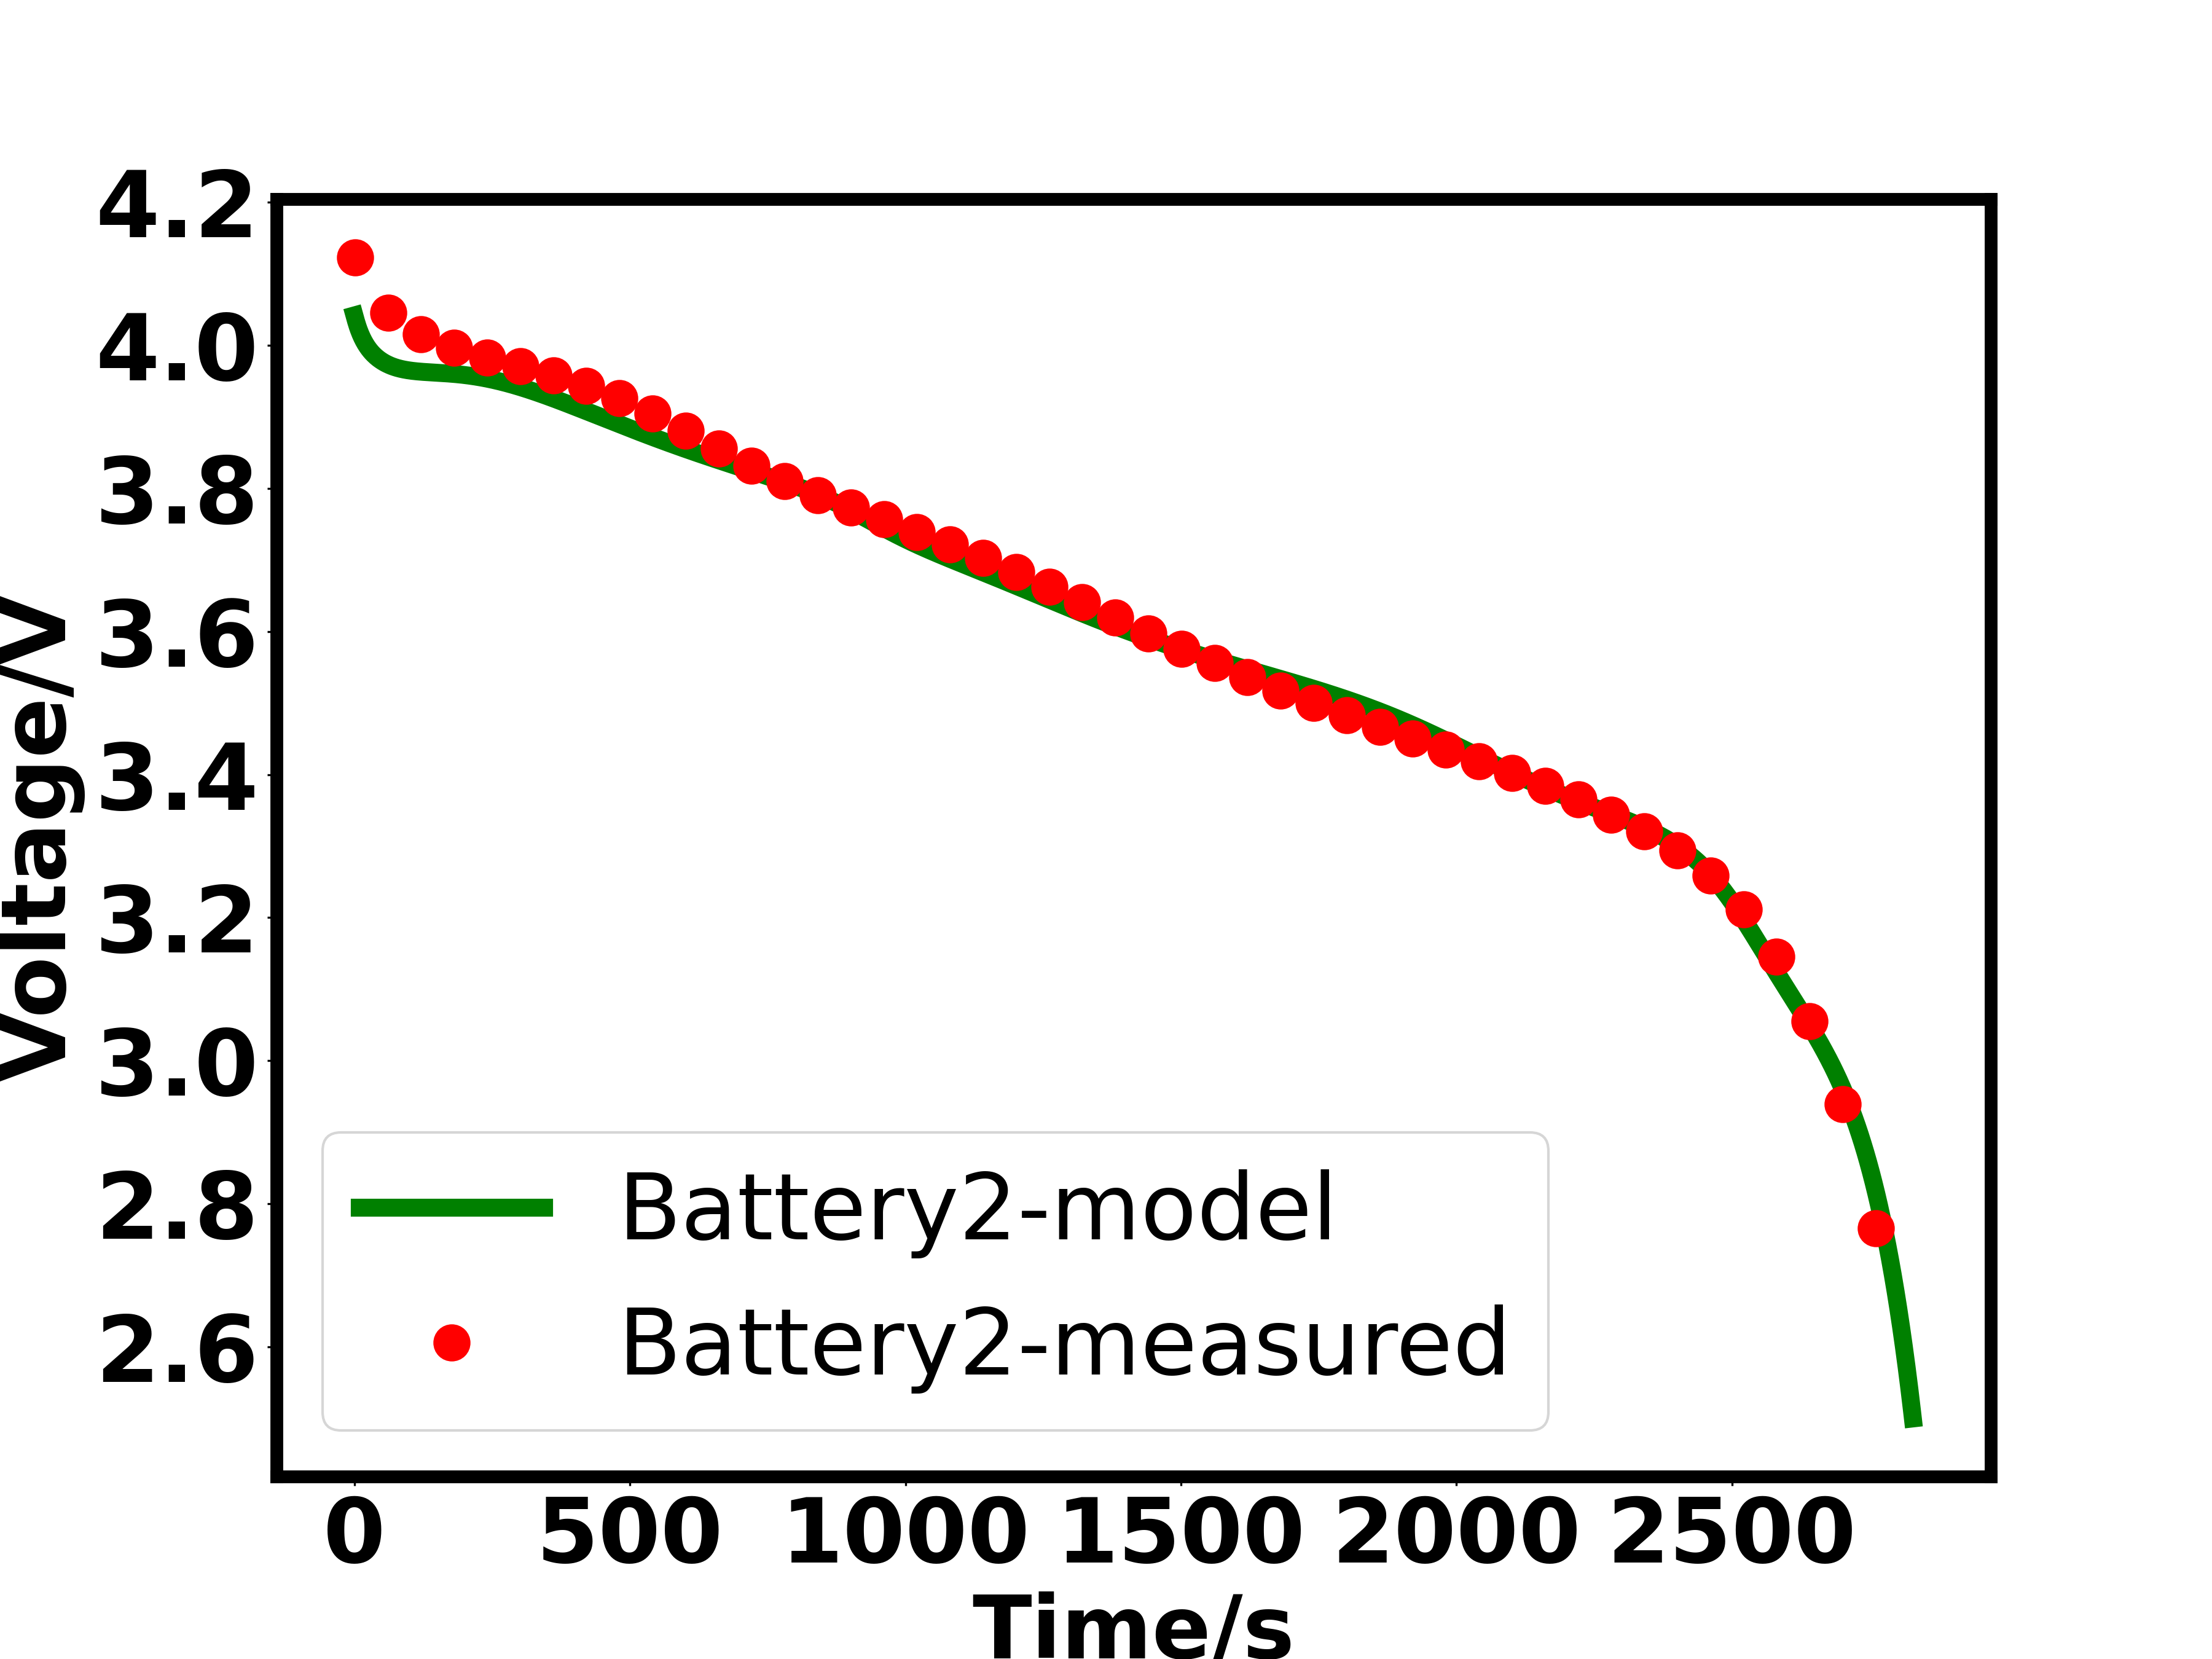
\includegraphics[width=\textwidth]{image/Battery2_volt.png}
        \caption{}
    \end{subfigure}
    \hfill
    \begin{subfigure}[t]{0.24\textwidth}
        \centering
        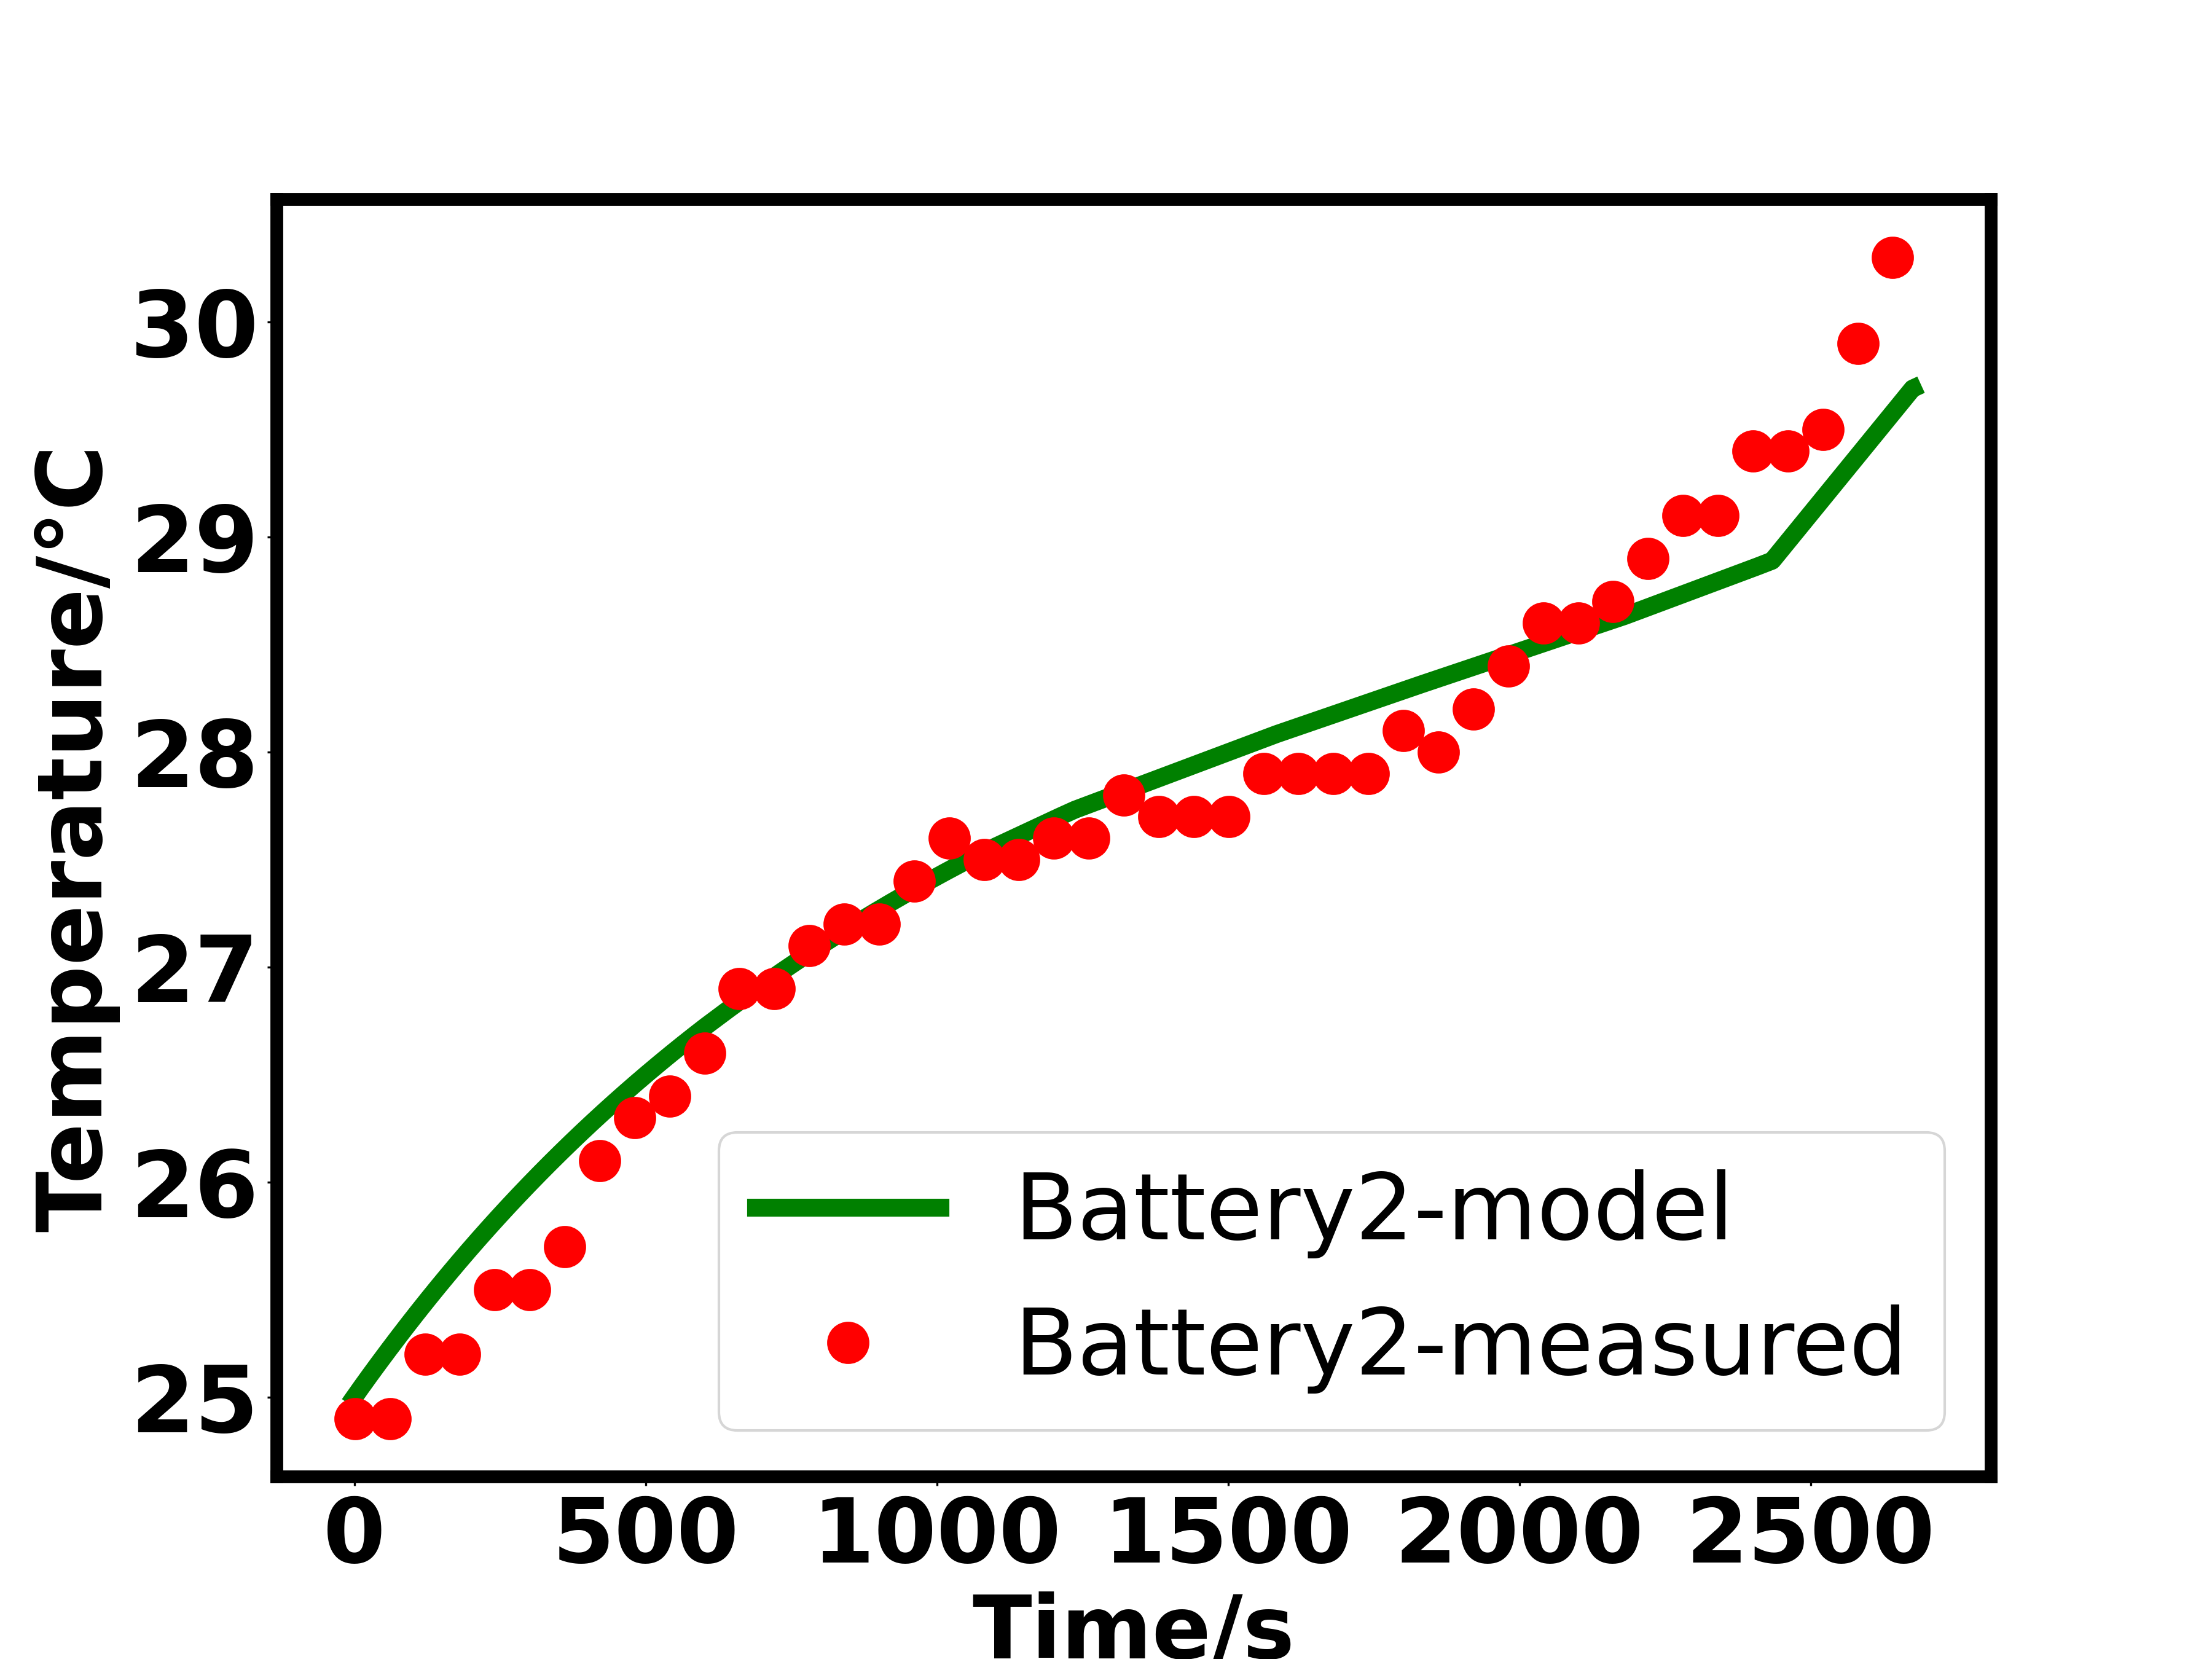
\includegraphics[width=\textwidth]{image/Battery2_temp.png} 
        \caption{}
    \end{subfigure}

    \caption{Parameter identification results for $Battery\;2$. (a) Electrochemical model parameter identification. (b) Thermal model parameter identification.}
    \label{battery2}
\end{figure}

\begin{figure}[t]
    \centering

    \begin{subfigure}[t]{0.24\textwidth} 
        \centering
        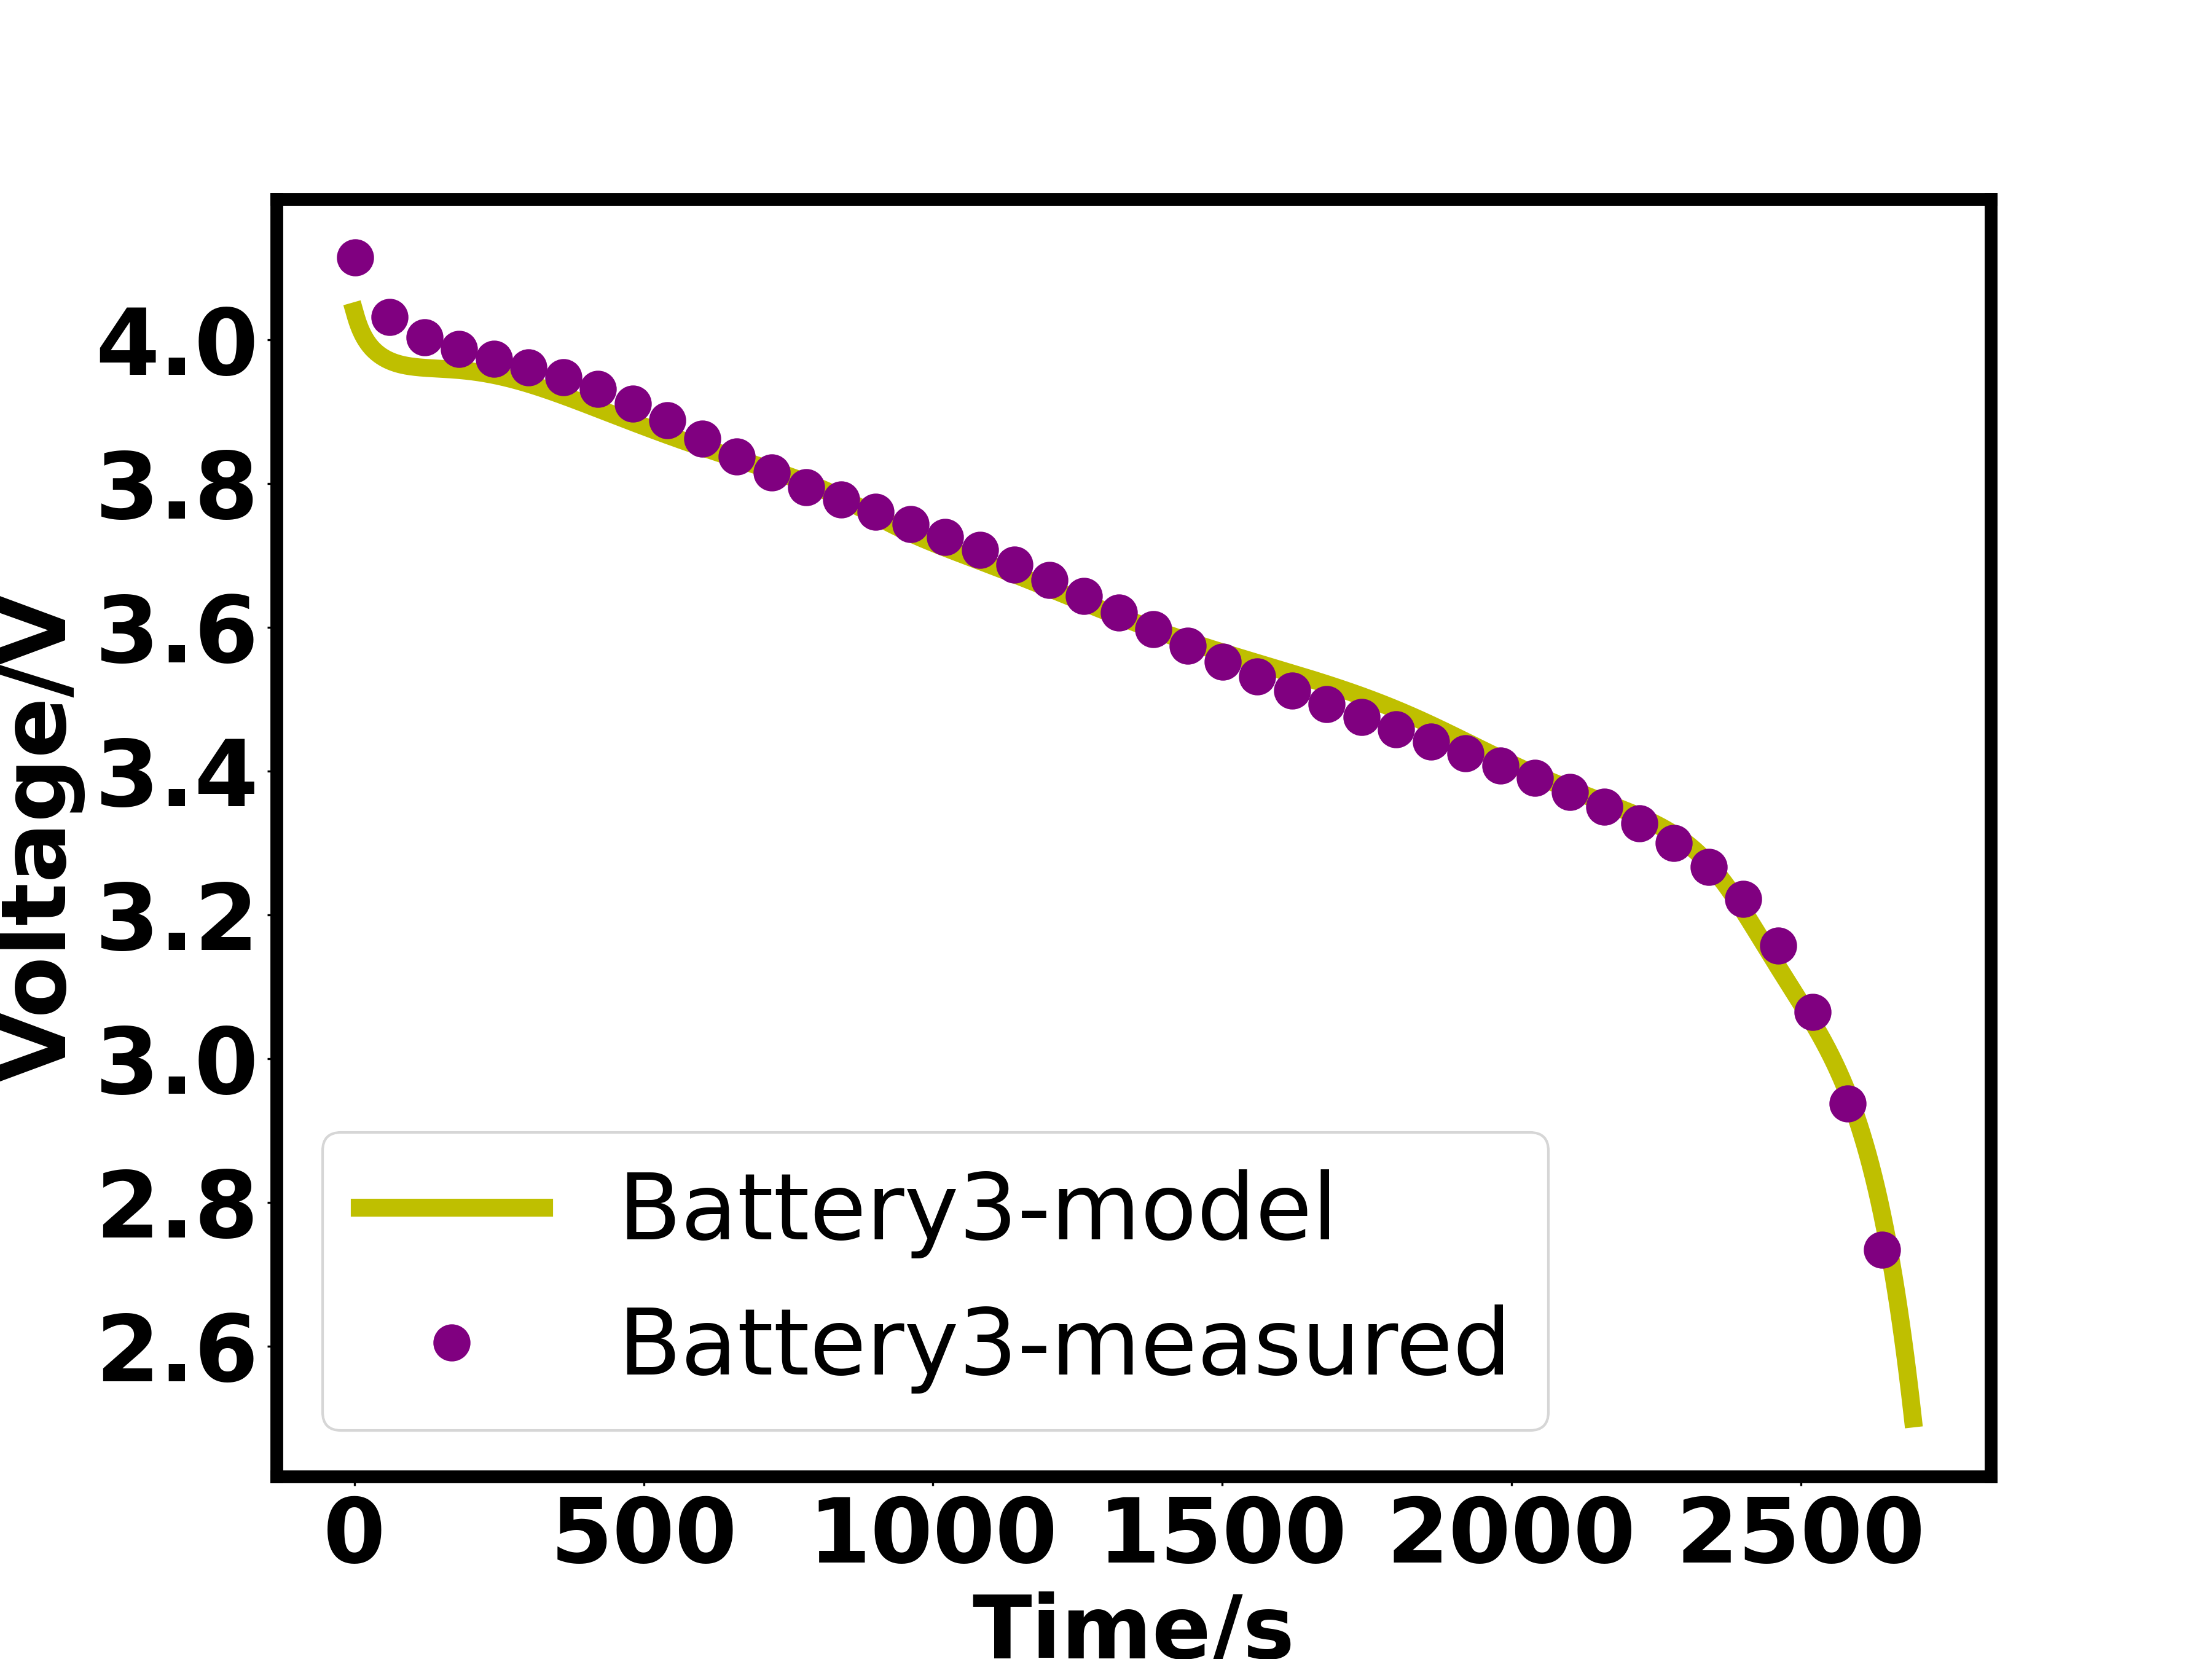
\includegraphics[width=\textwidth]{image/Battery3_volt.png}
        \caption{}
    \end{subfigure}
    \hfill
    \begin{subfigure}[t]{0.24\textwidth}
        \centering
        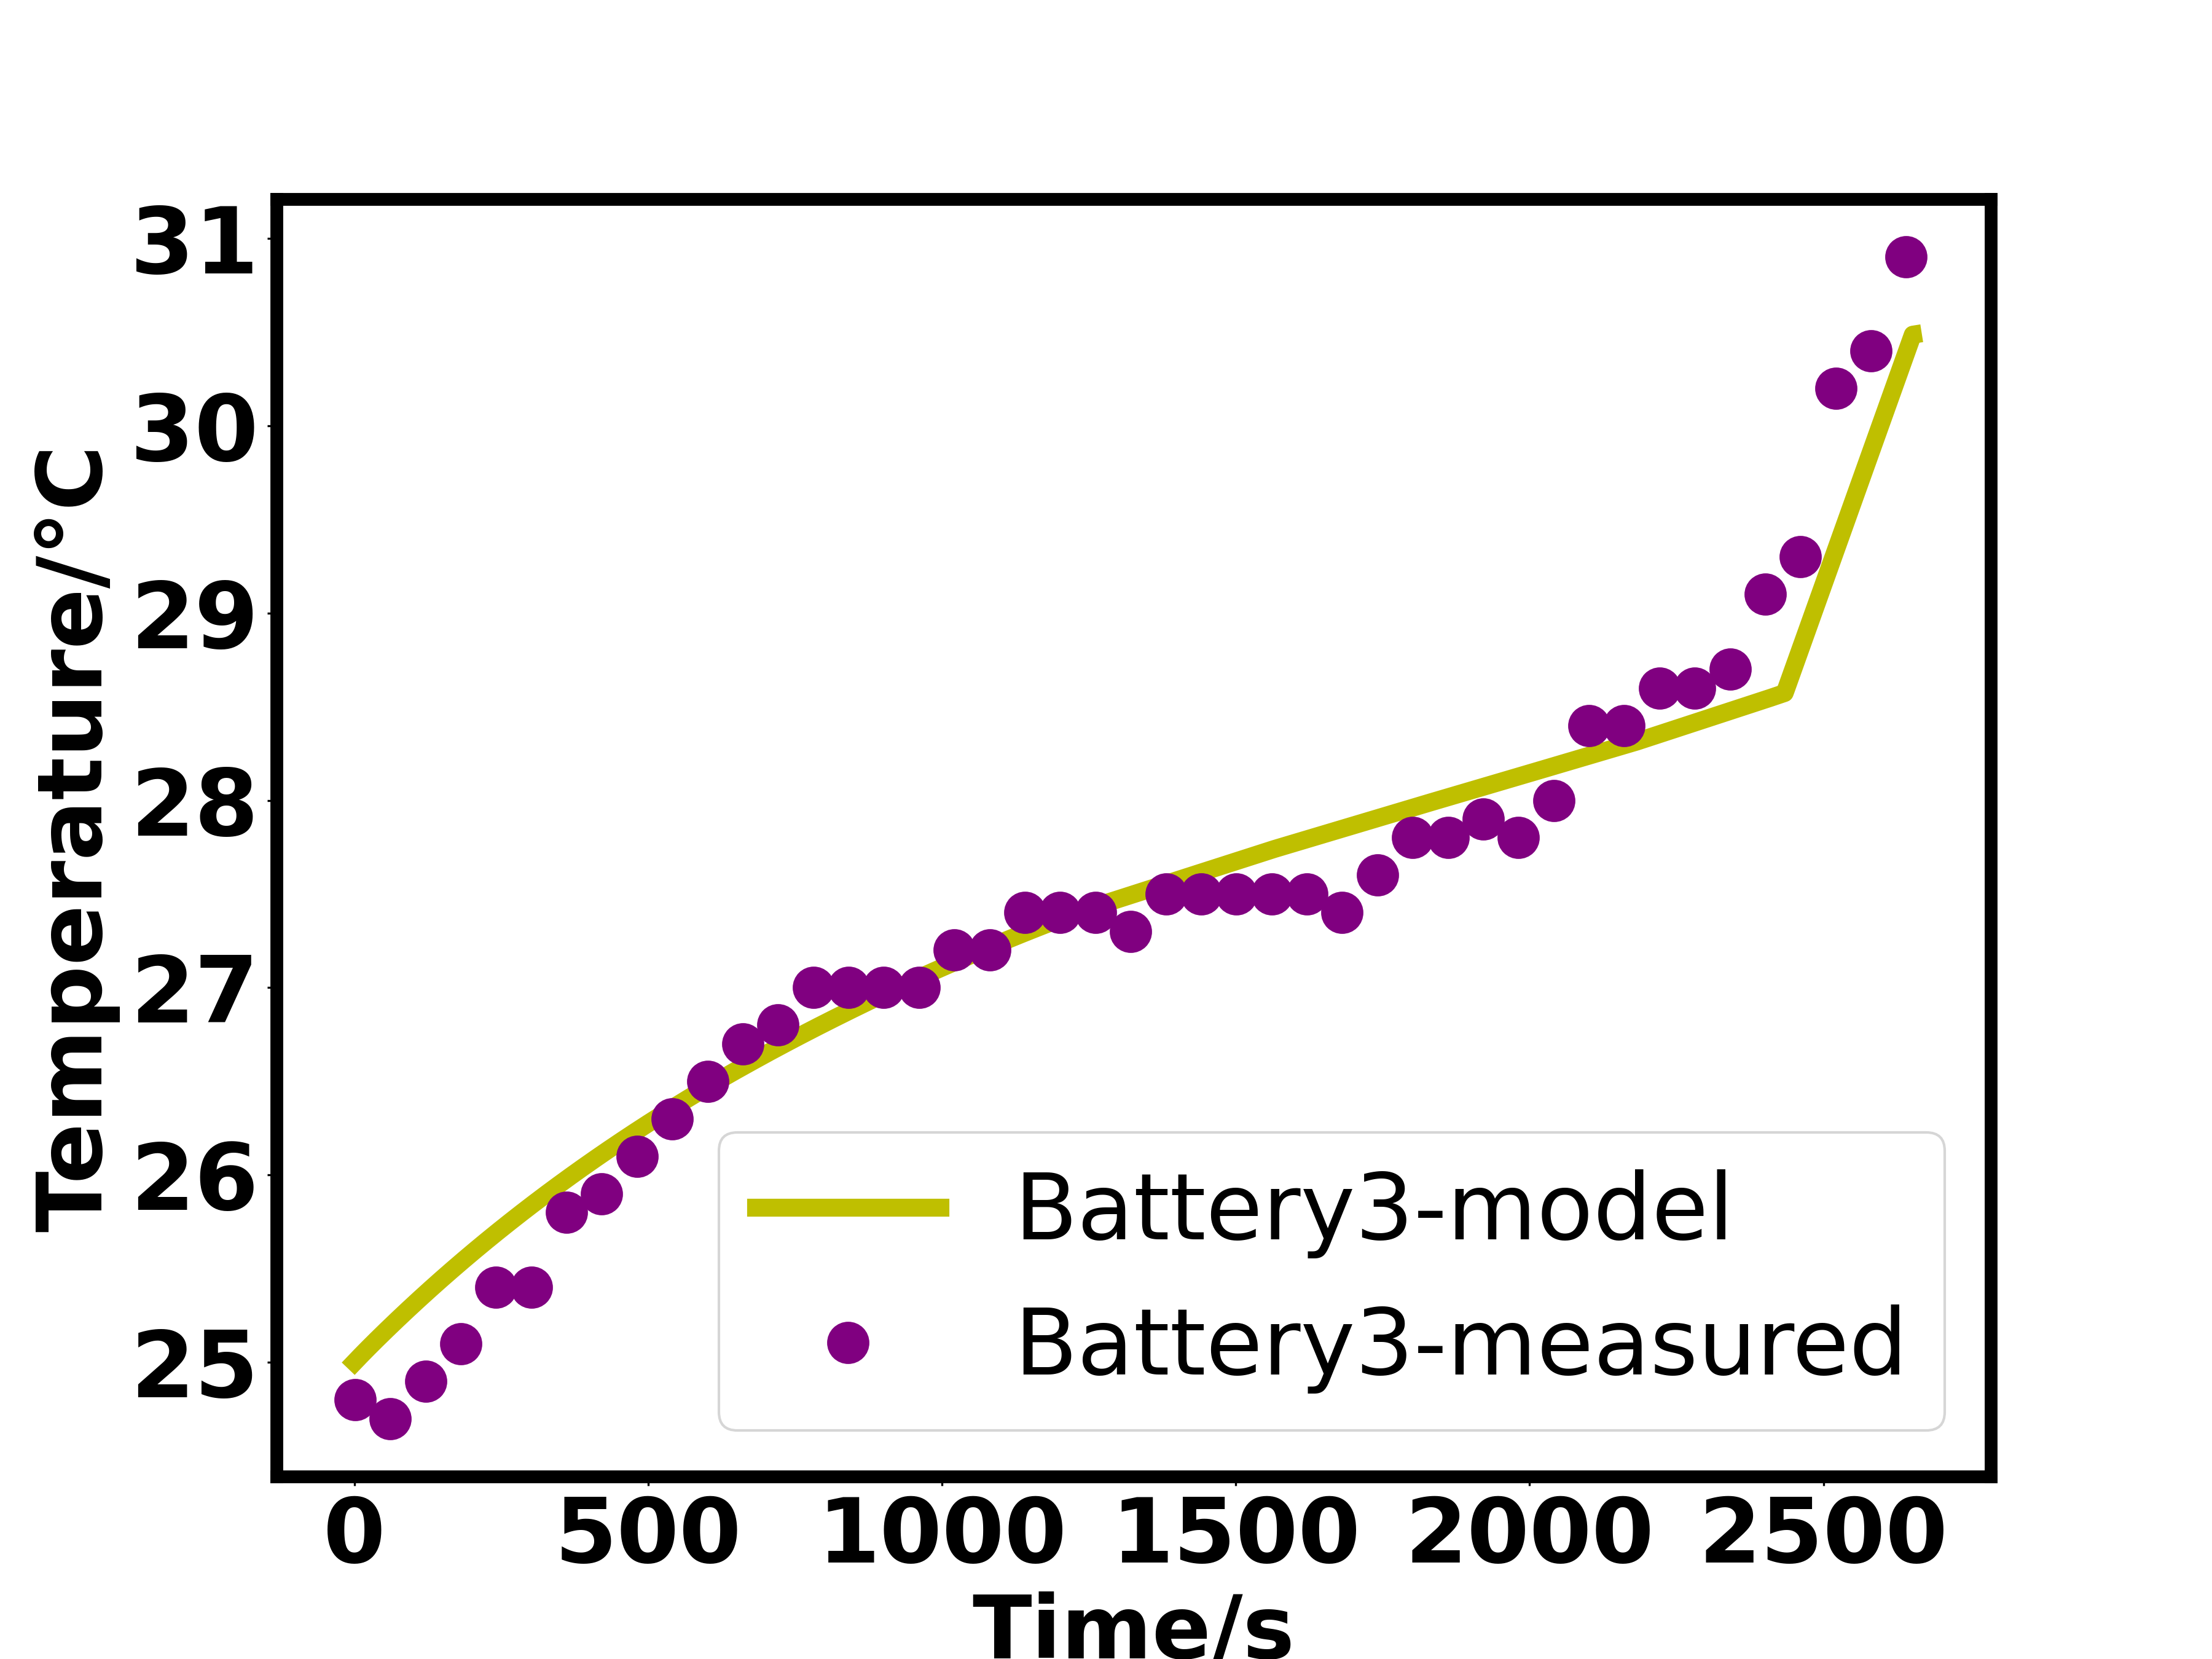
\includegraphics[width=\textwidth]{image/Battery3_temp.png} 
        \caption{}
    \end{subfigure}

    \caption{Parameter identification results for $Battery\;3$. (a) Electrochemical model parameter identification. (b) Thermal model parameter identification.}
    \label{battery3}
\end{figure}

\section{Results and Discussions}
The performance of the MBA-RL framework was evaluated in this section. Three Samsung 40T 21700 batteries, denoted as $Battery\;1$, $Battery\;2$, and $Battery\;3$, were used in this study. These are high-performance cylindrical lithium-ion batteries with a nominal capacity of 4000 mAh and a maximum discharge rate of 35 A. In the experimental process, real-world data were initially gathered from the experimental platform, as outlined in Fig.~\ref{fig:experiment_Schematic}. Parameter identification was then performed using the PSO algorithm. This step seeks to model the variability in battery lifespans across different cells, providing a more authentic representation of practical scenarios. Furthermore, a system comprised of batteries with varying levels of degradation presents a more rigorous test for the control framework, thereby strengthening the robustness of the proposed method. Then, we validated the effectiveness of the MBA-RL framework on the NEWARE CT-4008-5V20A-A battery testing equipment, which enables the input of different charging currents to individual cells, thus eliminating the need for an equalization topology. In addition, we compared the MBA-RL framework against two methods: a single-agent deep Q-learning (DQL) method and the CC-CV method, both of which rely on the cell-to-cell topology from \cite{ghaeminezhad2021active}. Additionally, the multiple batteries involved in this paper were subjected to charge and discharge experiments in a laboratory environment. The batteries were connected in parallel, a configuration that ensures different currents are directed to individual batteries.

\begin{figure*}[htbp]
    \centering
        \begin{subfigure}[t]{0.32\textwidth}
        \centering
        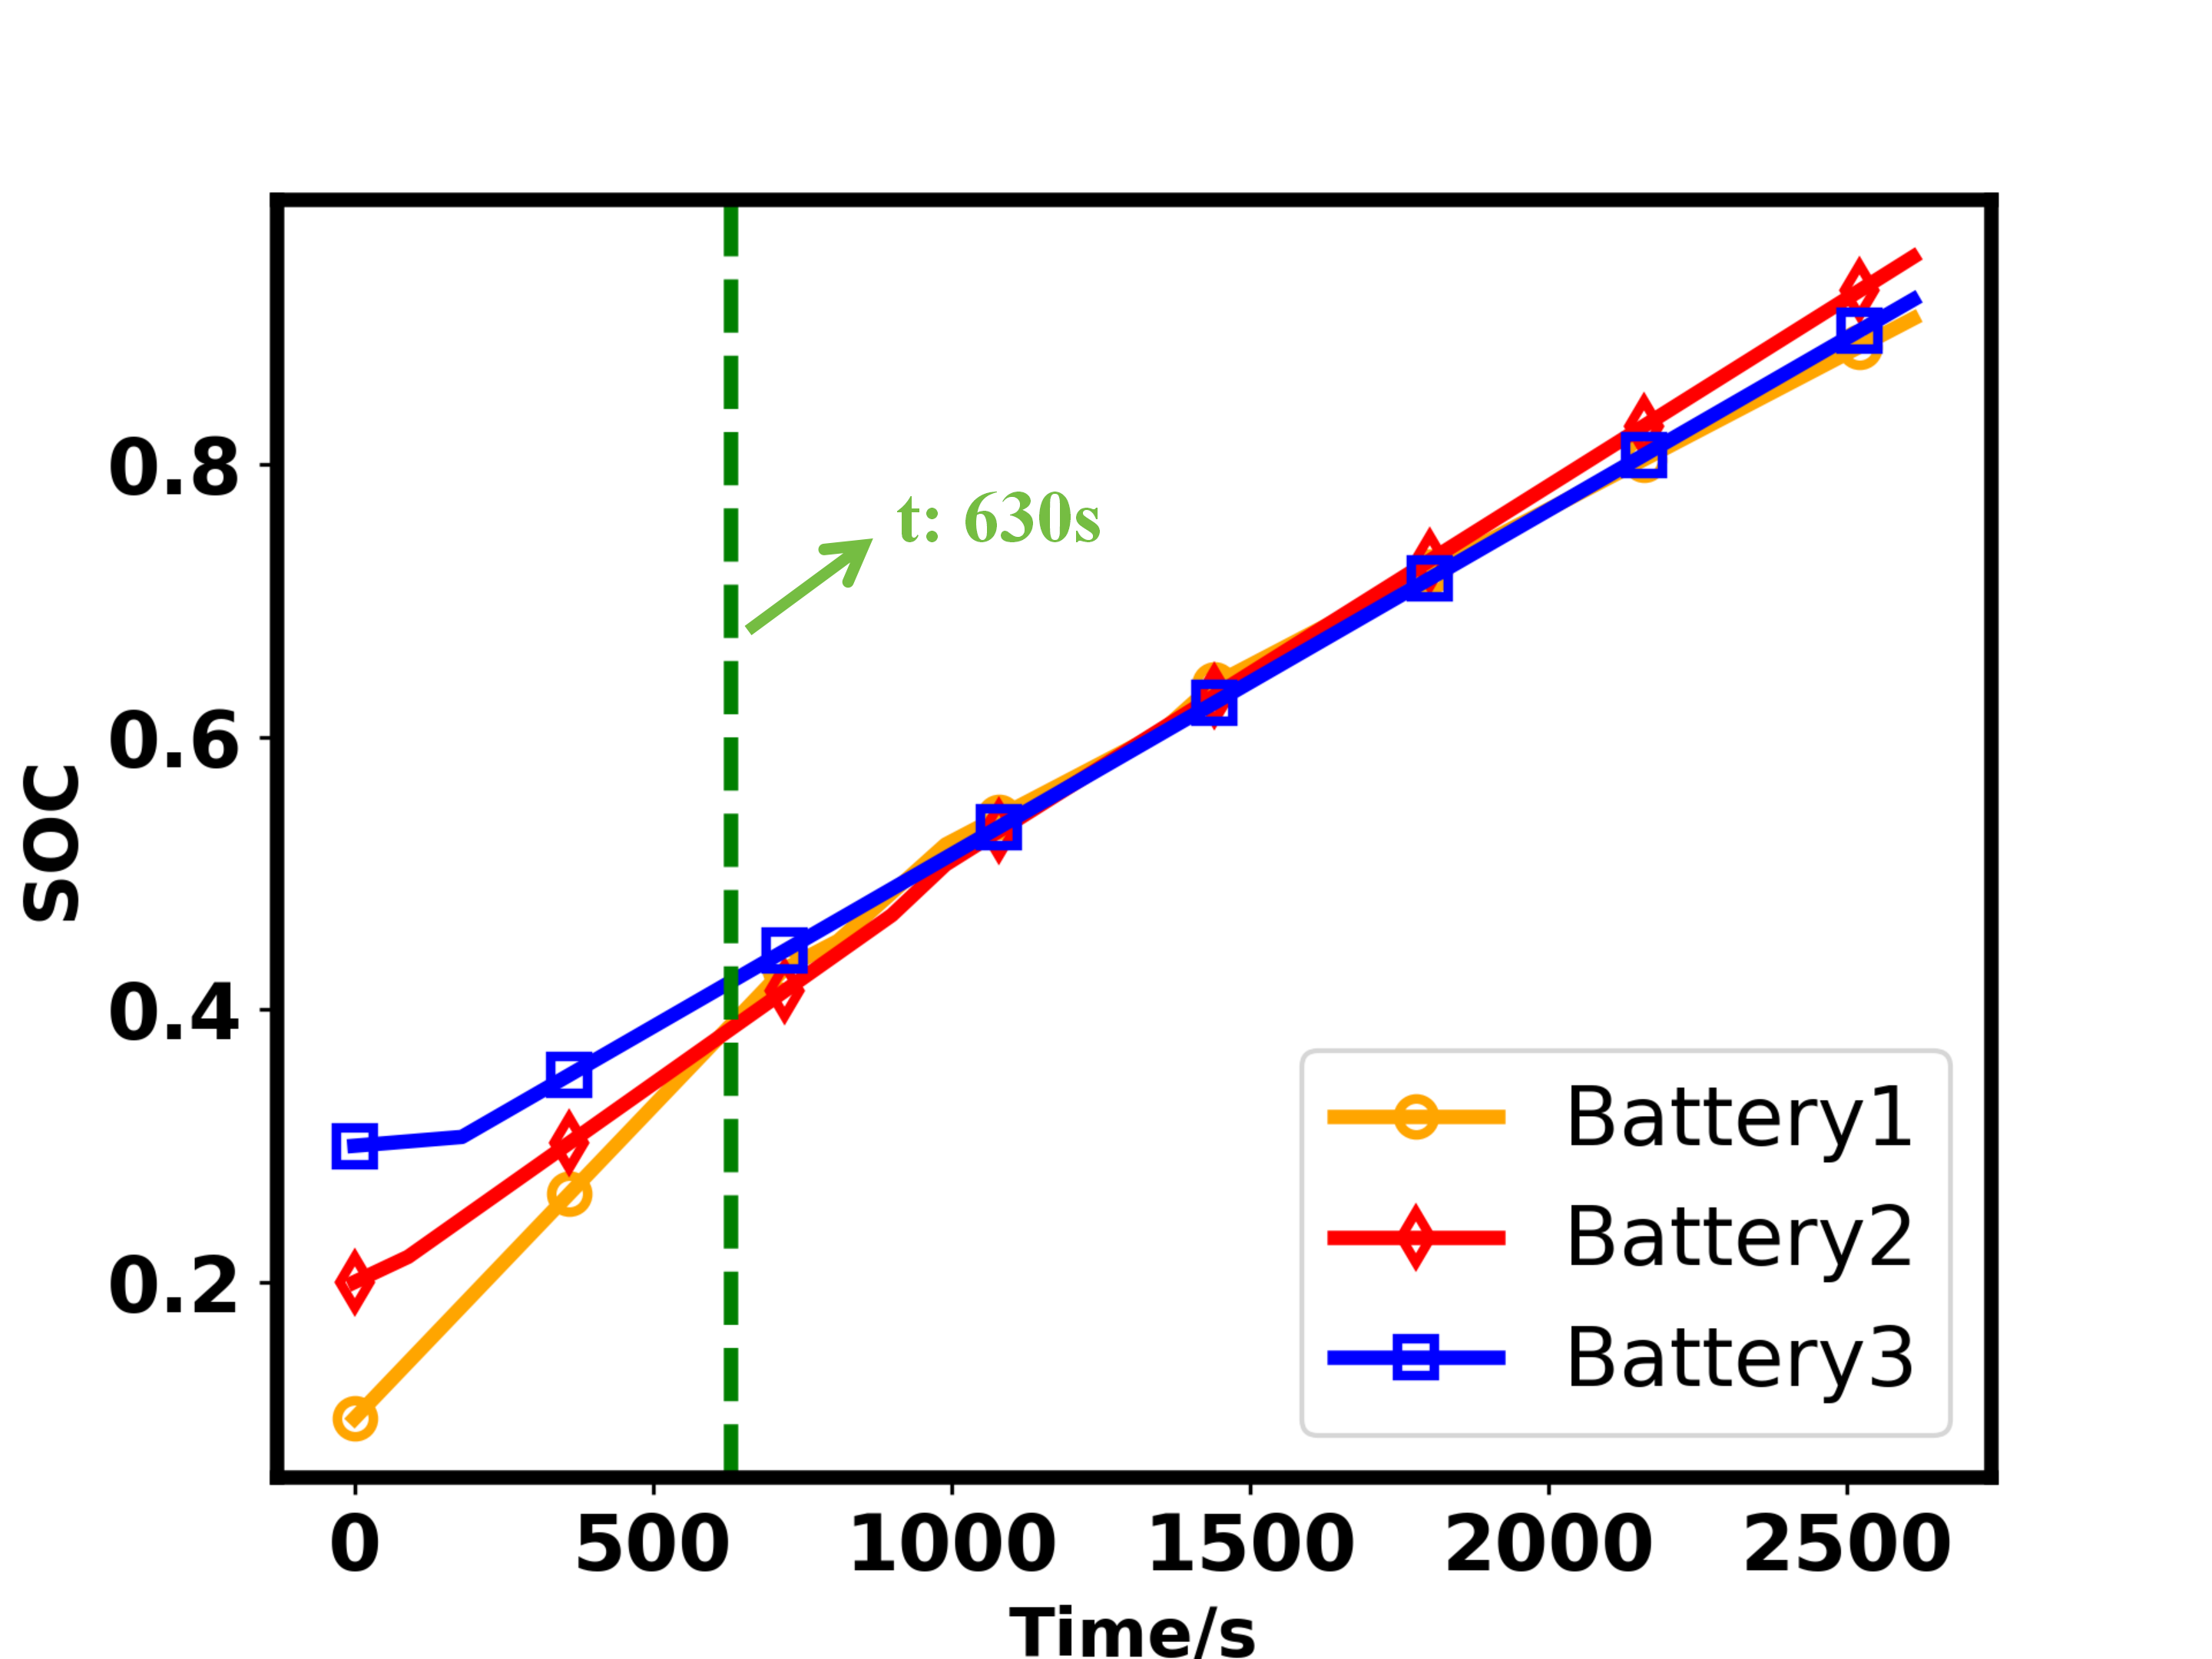
\includegraphics[width=\textwidth]{image/MBA_RL 0.1 0.2 0.3.png}
        \caption{}
    \end{subfigure}
    \hfill
        \begin{subfigure}[t]{0.32\textwidth} 
        \centering
        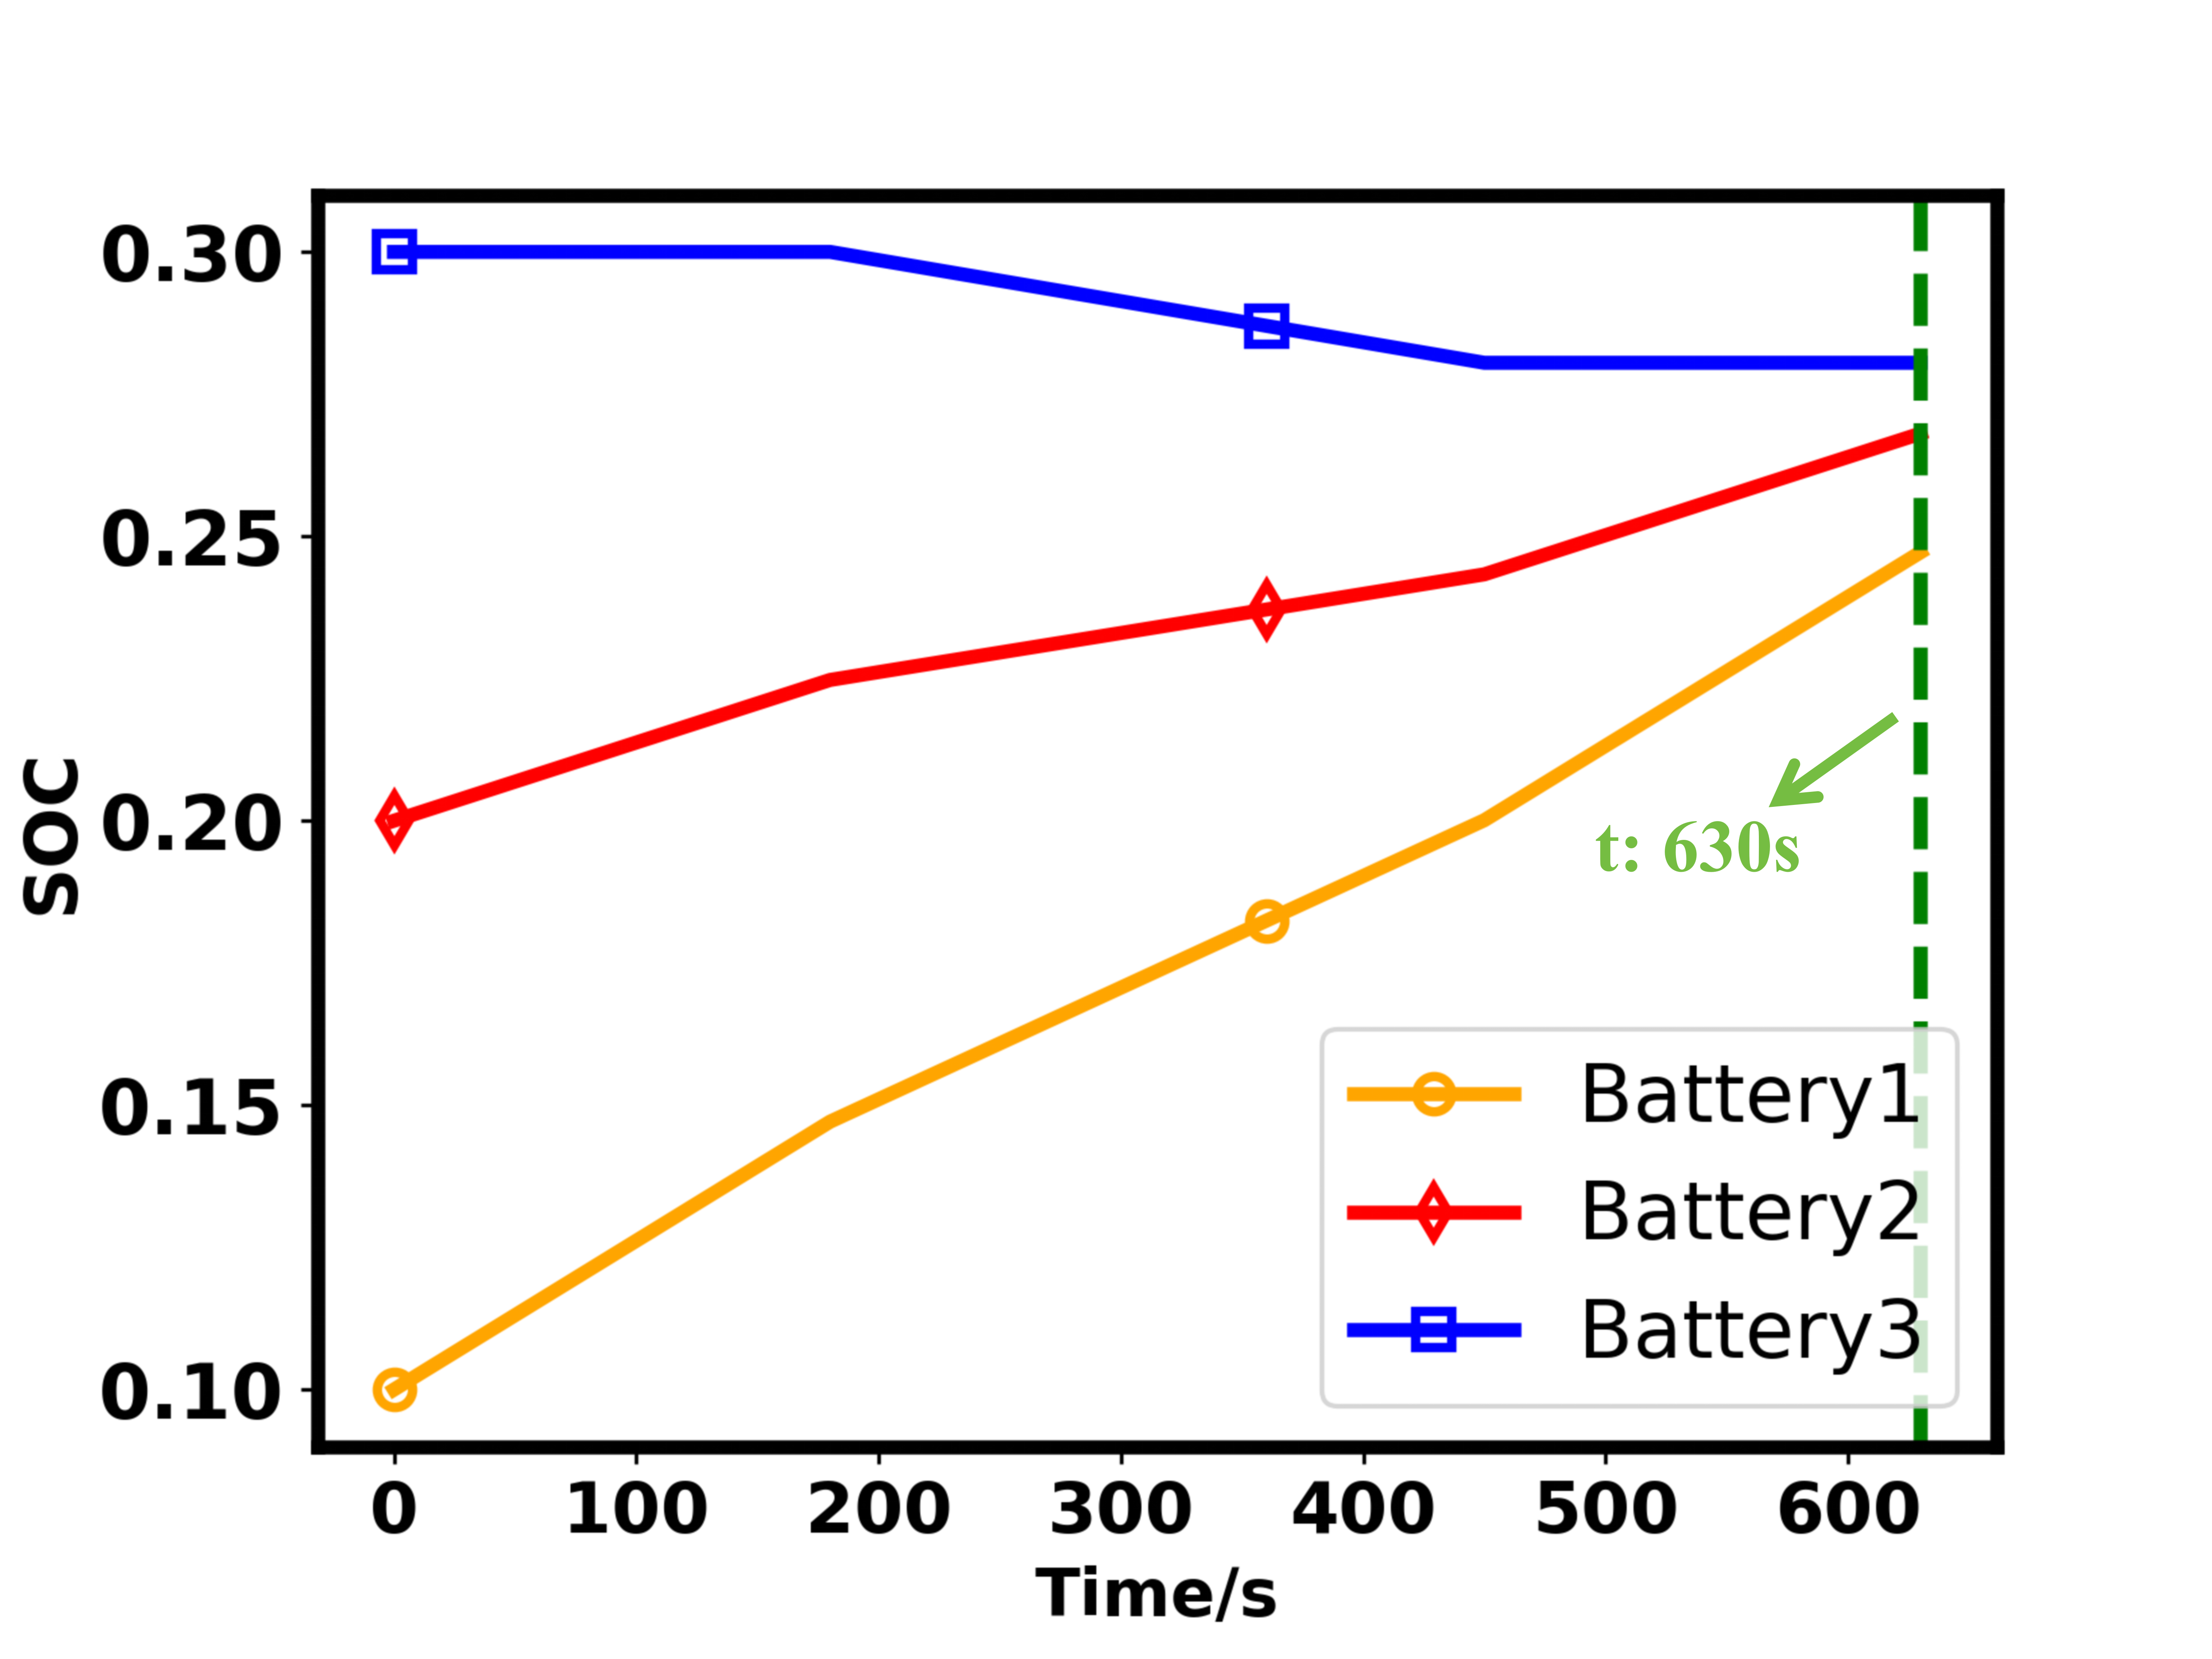
\includegraphics[width=\textwidth]{image/DQN 0.1 0.2 0.3.png}
        \caption{}
    \end{subfigure}
    \hfill
        \begin{subfigure}[t]{0.32\textwidth} 
        \centering
        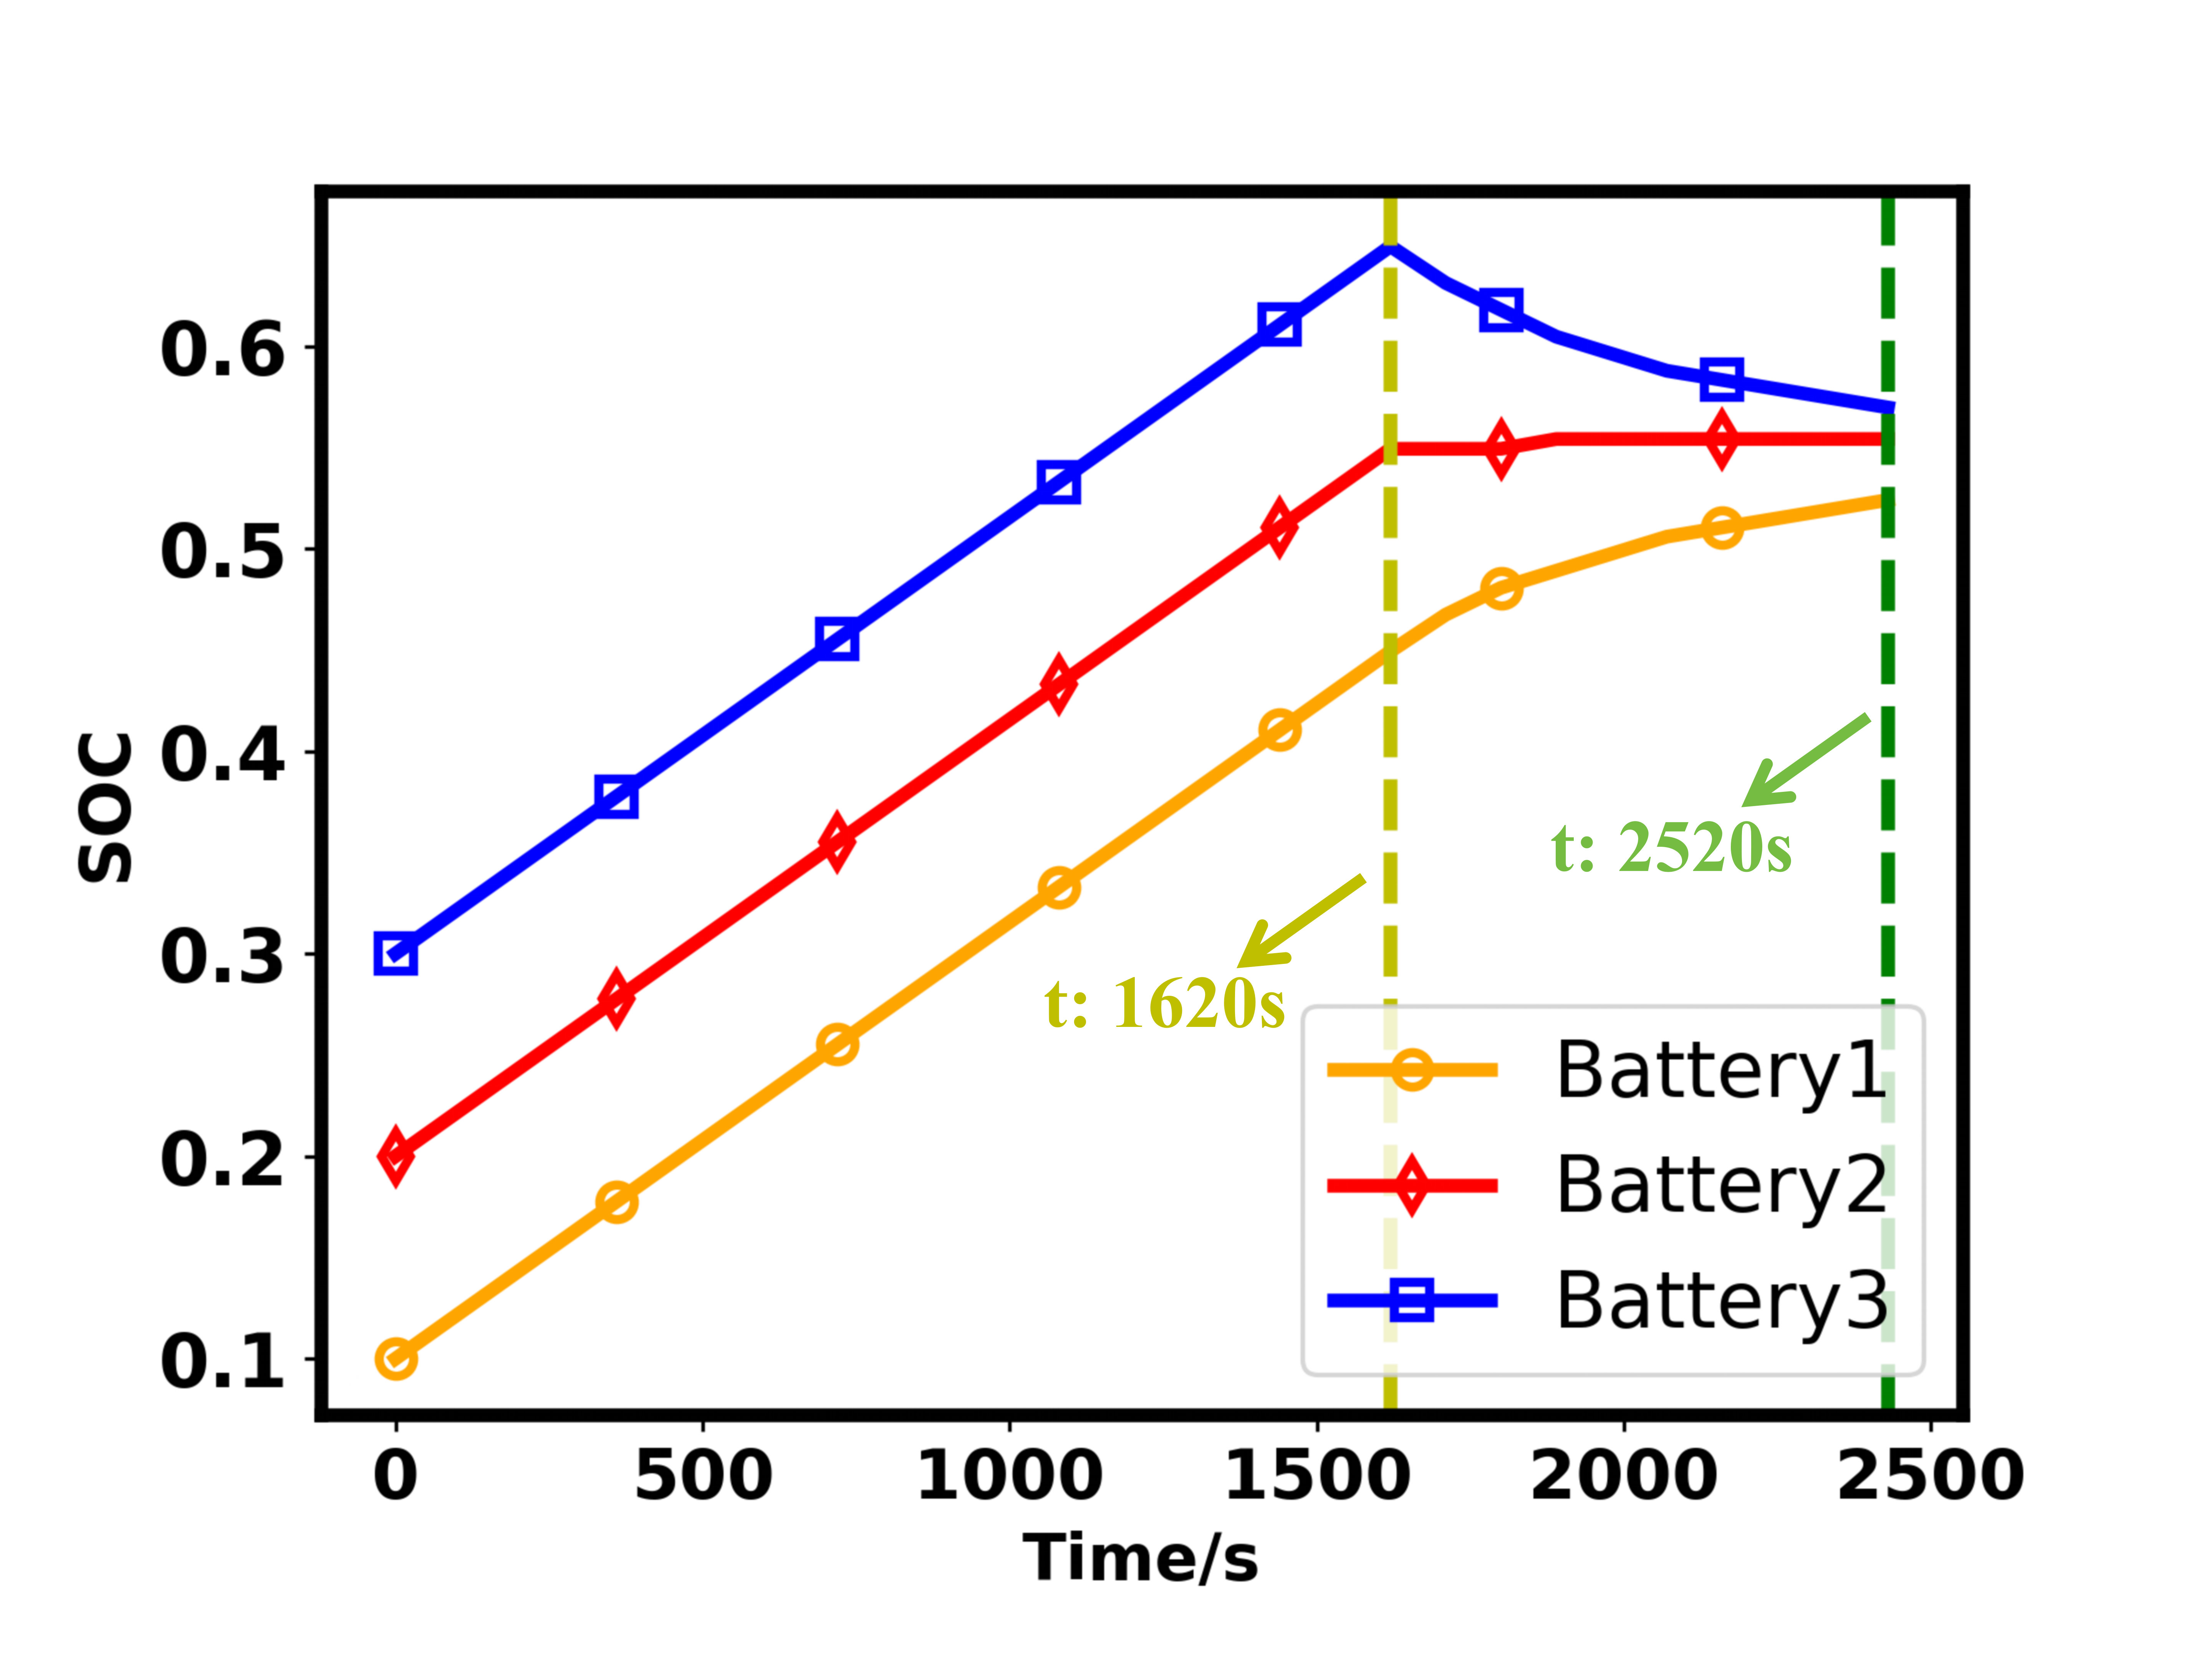
\includegraphics[width=\textwidth]{image/CC-CV 0.1 0.2 0.3.png}
        \caption{}
    \end{subfigure}

    \vspace{0.1cm}

    \begin{subfigure}[t]{0.32\textwidth}
        \centering
        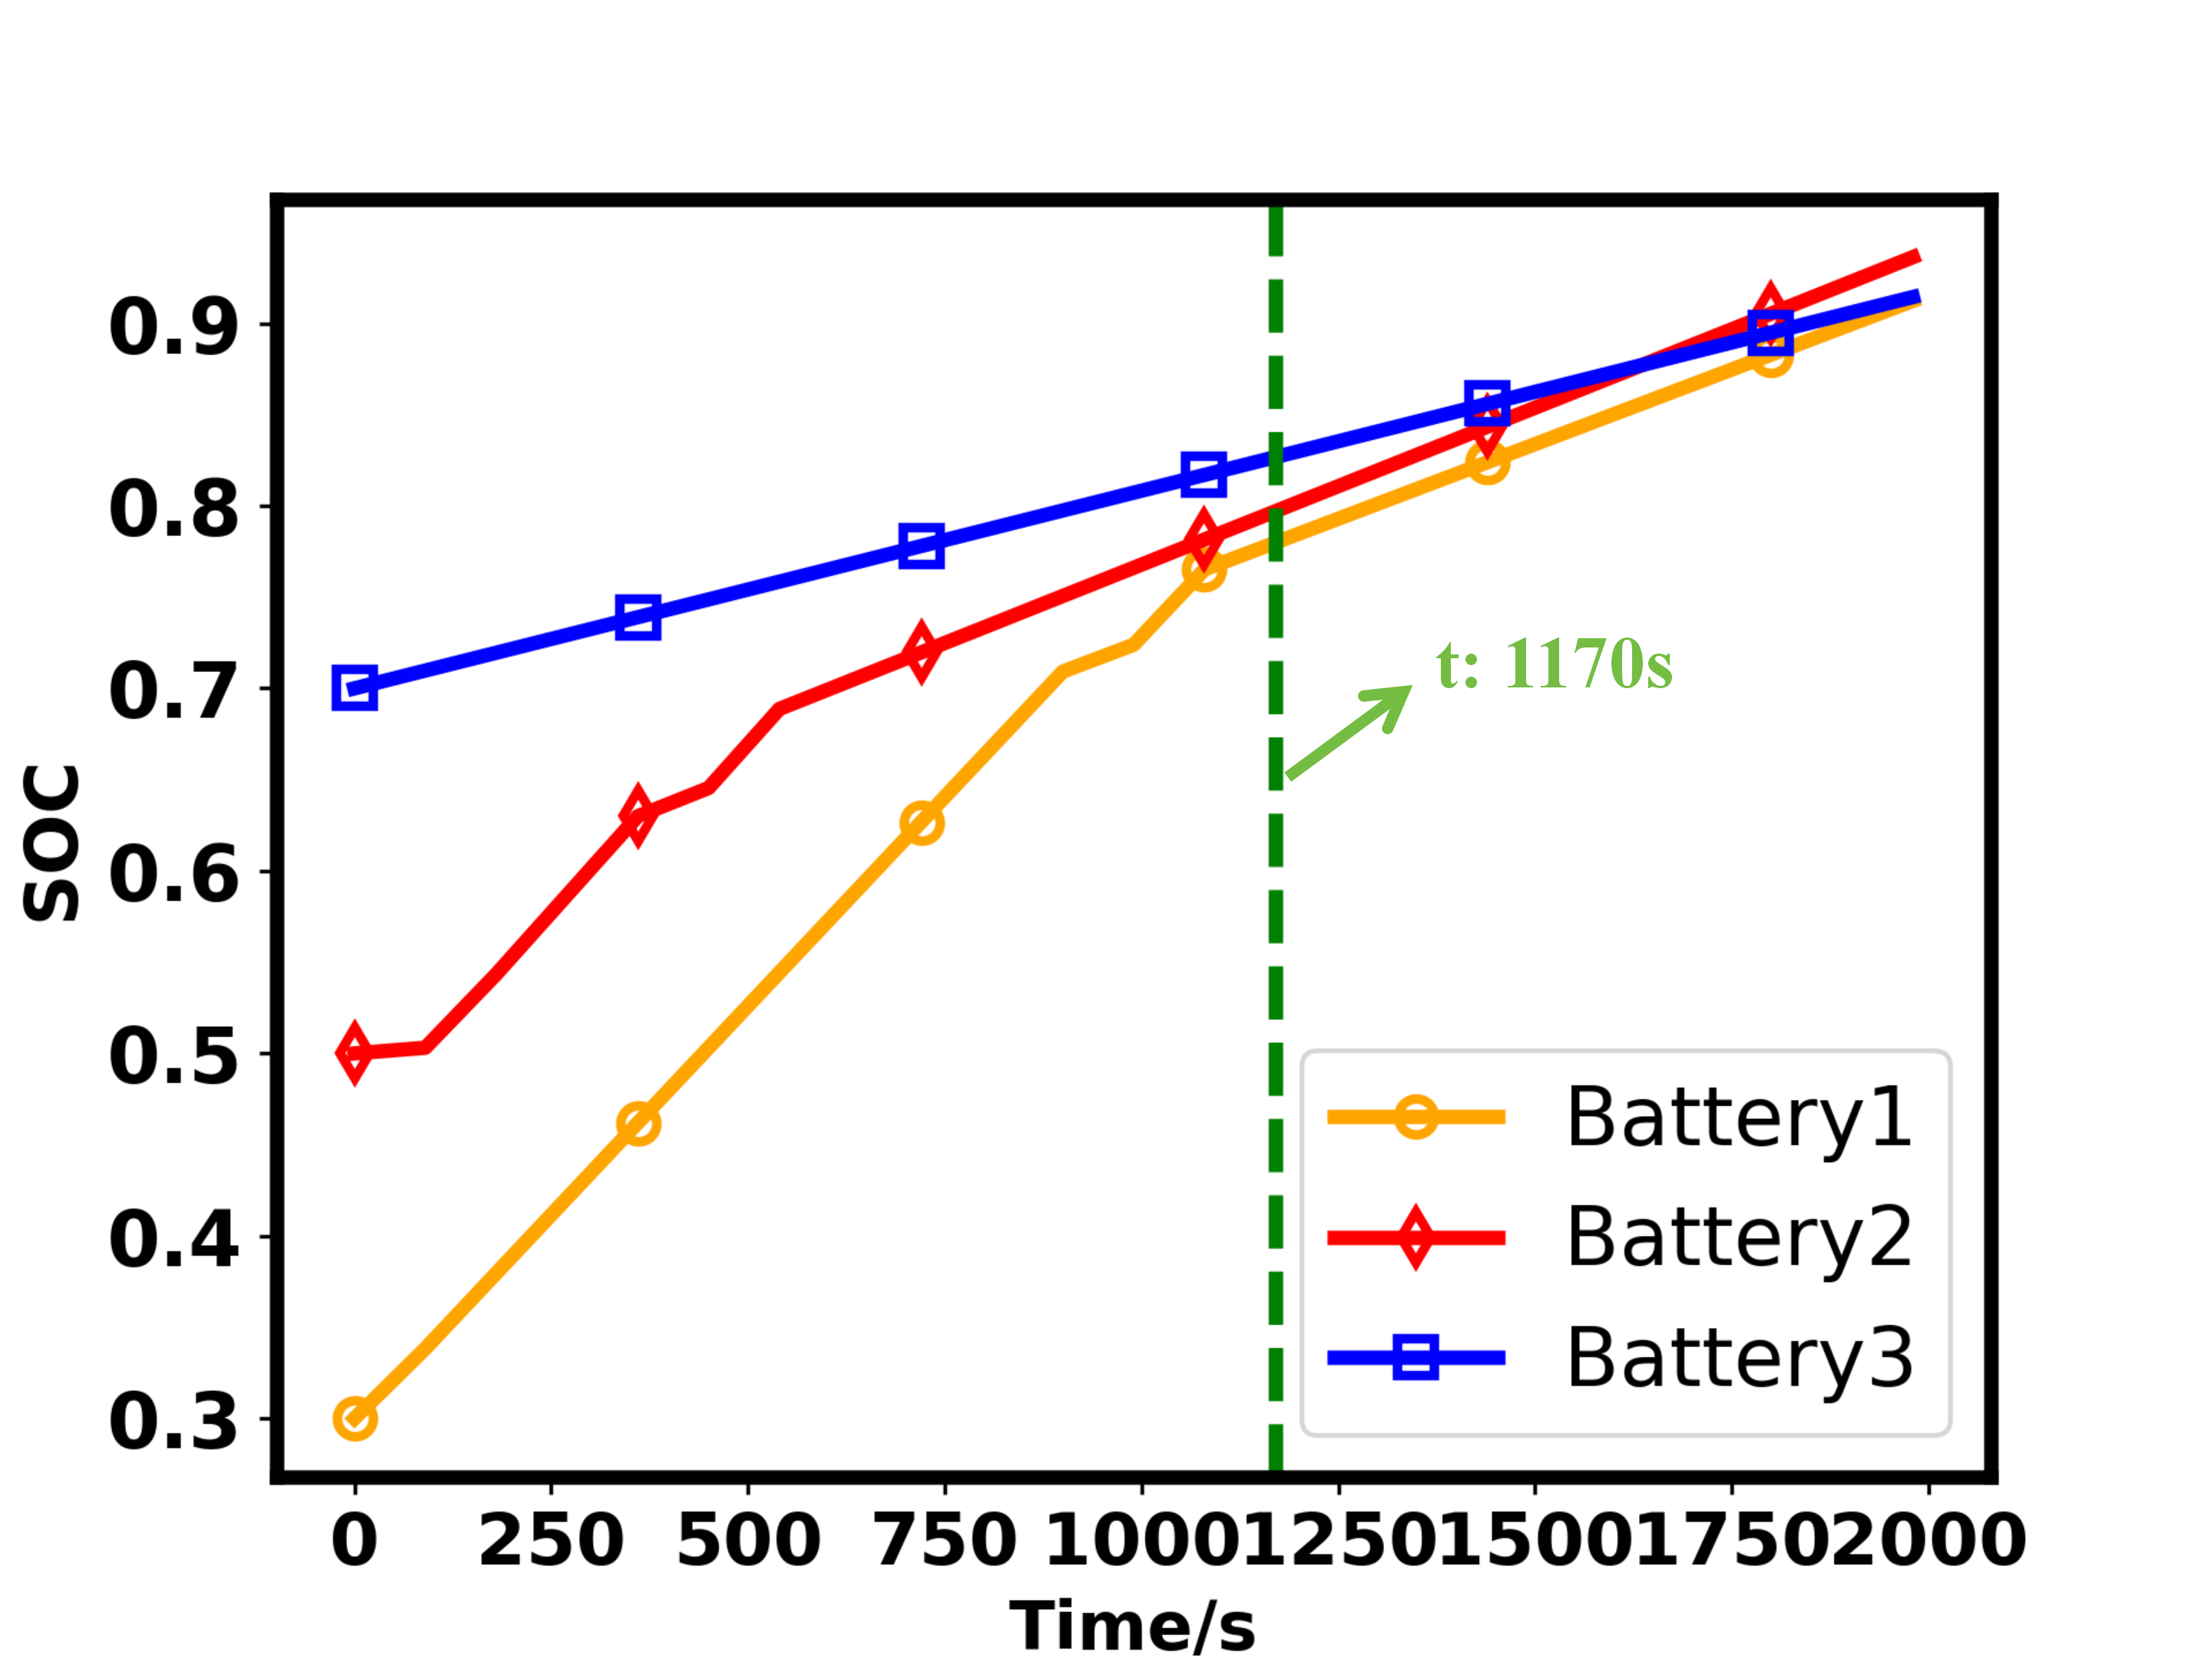
\includegraphics[width=\textwidth]{image/MBA_RL 0.3 0.5 0.7.png}
        \caption{}
    \end{subfigure}
    \hfill
    \begin{subfigure}[t]{0.32\textwidth}
        \centering
        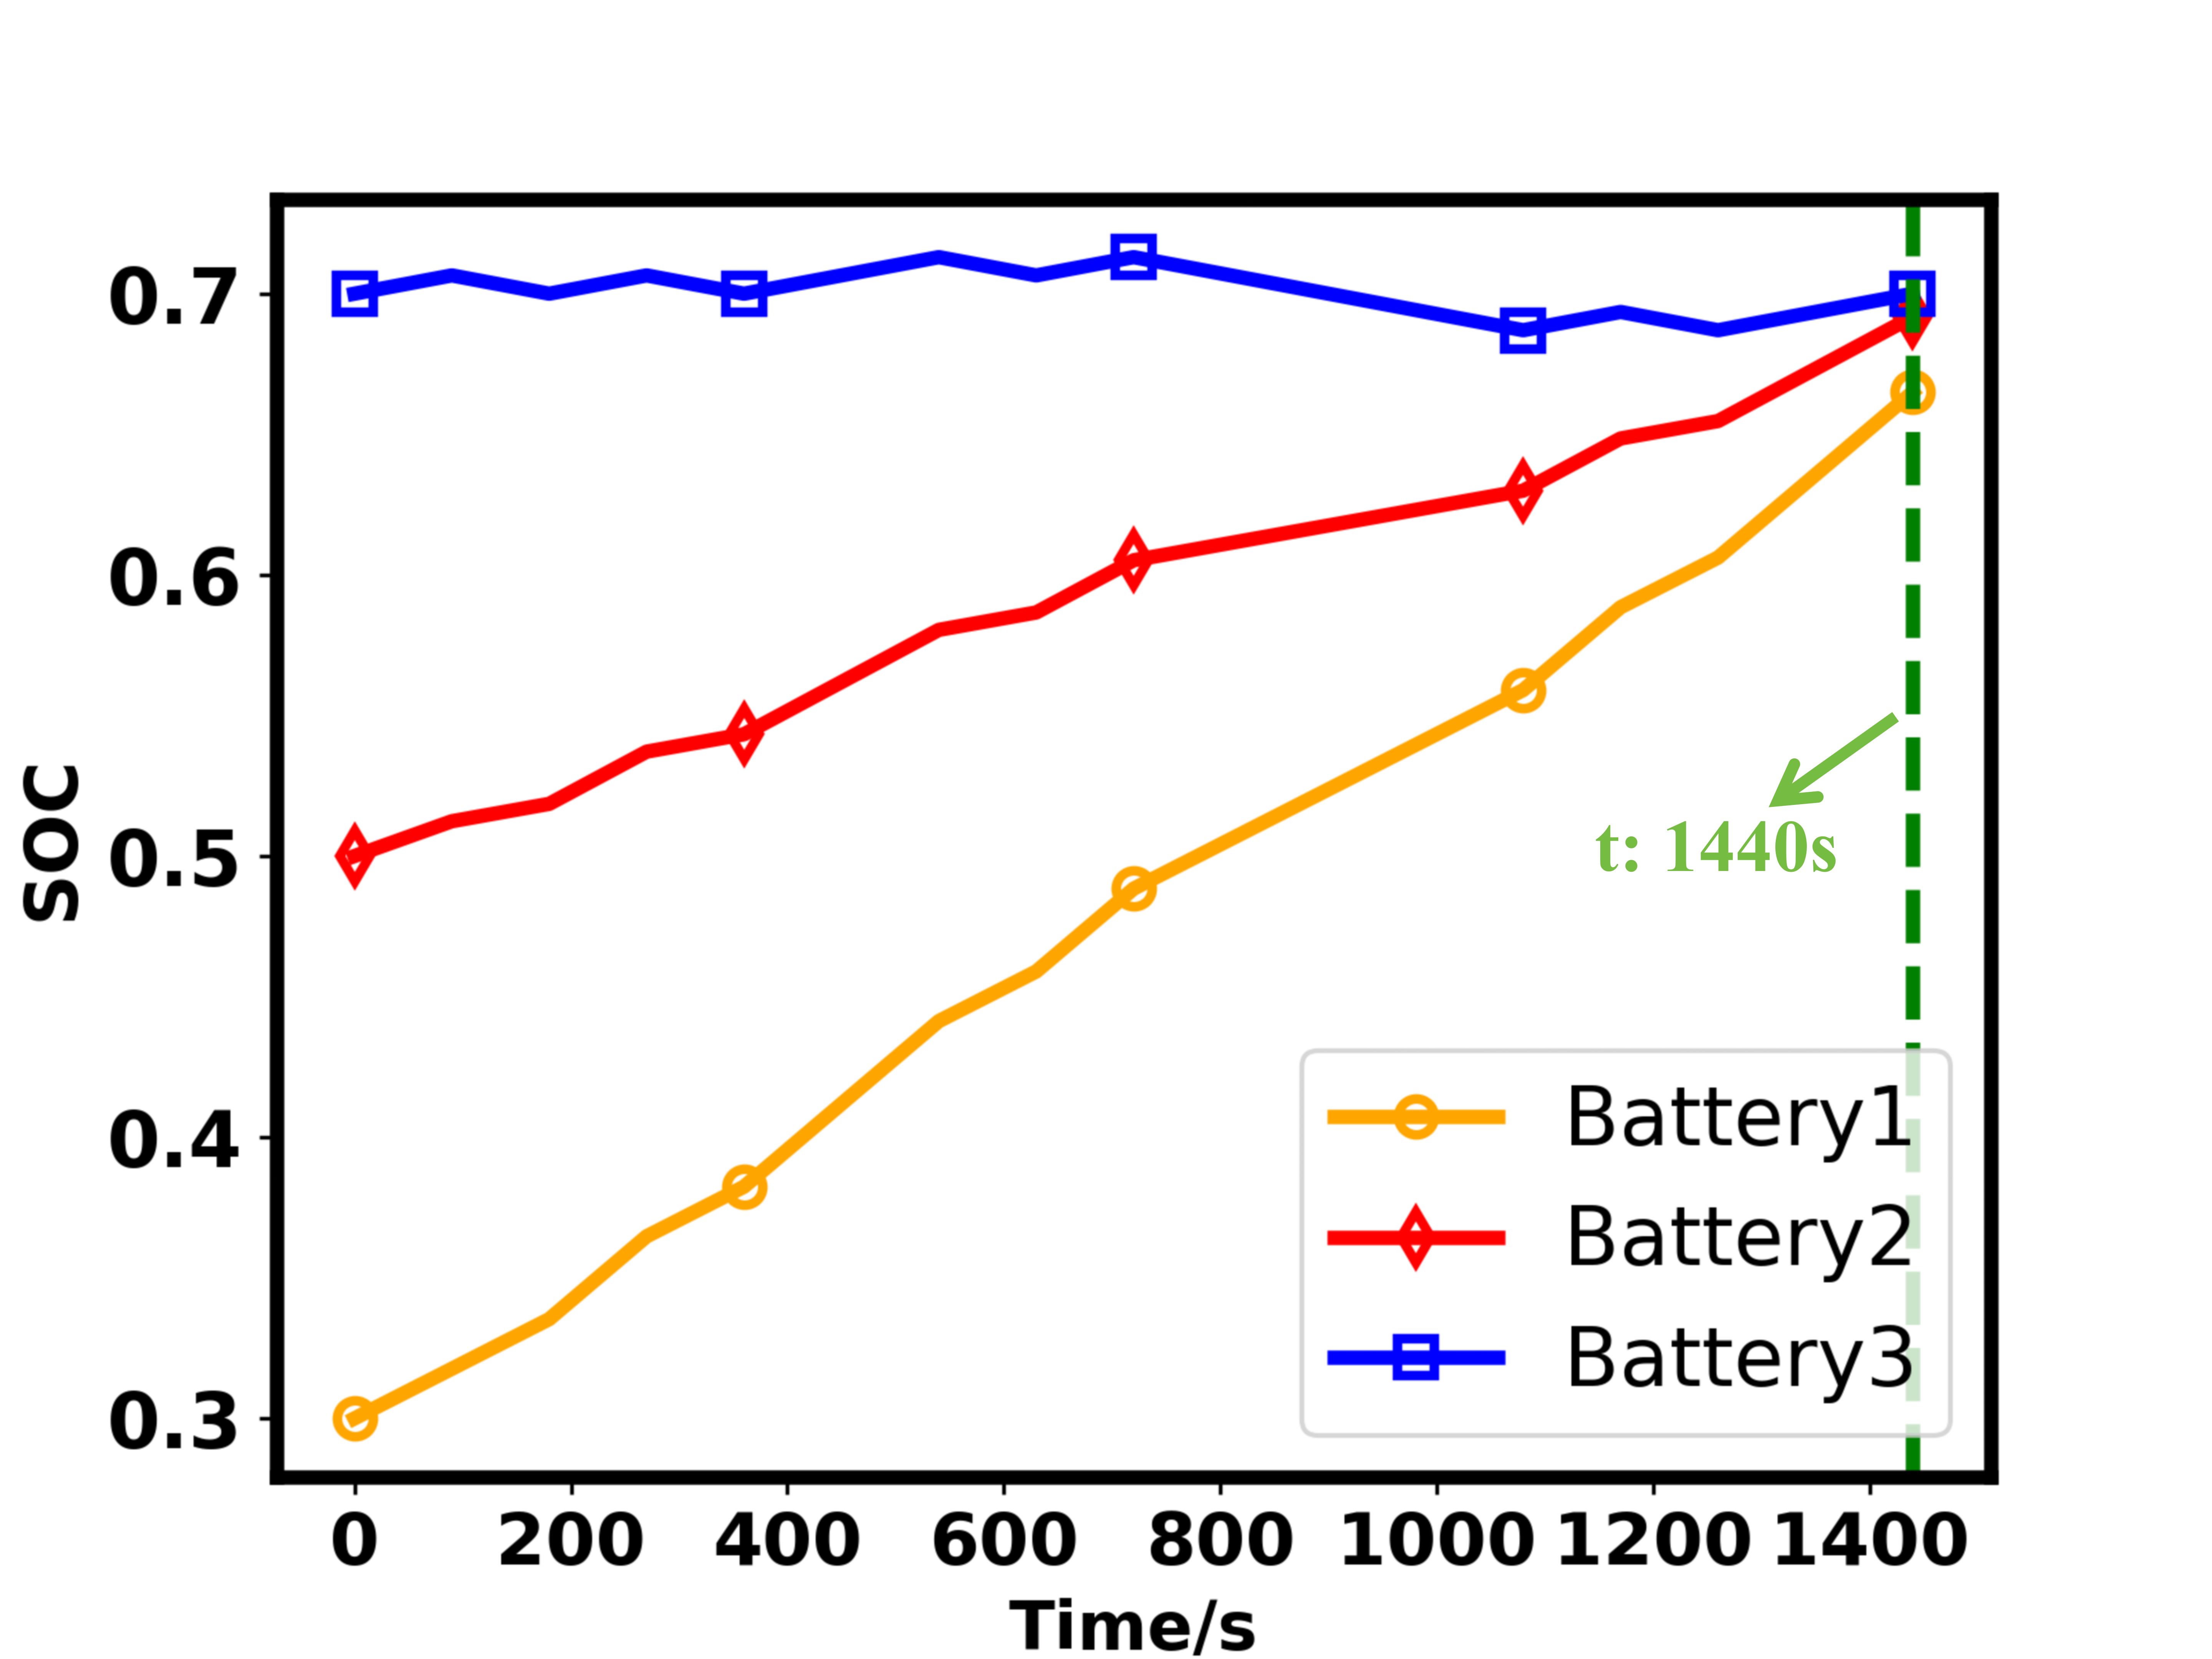
\includegraphics[width=\textwidth]{image/DQN 0.3 0.5 0.7.png}
        \caption{}
    \end{subfigure}
    \hfill
    \begin{subfigure}[t]{0.32\textwidth} 
        \centering
        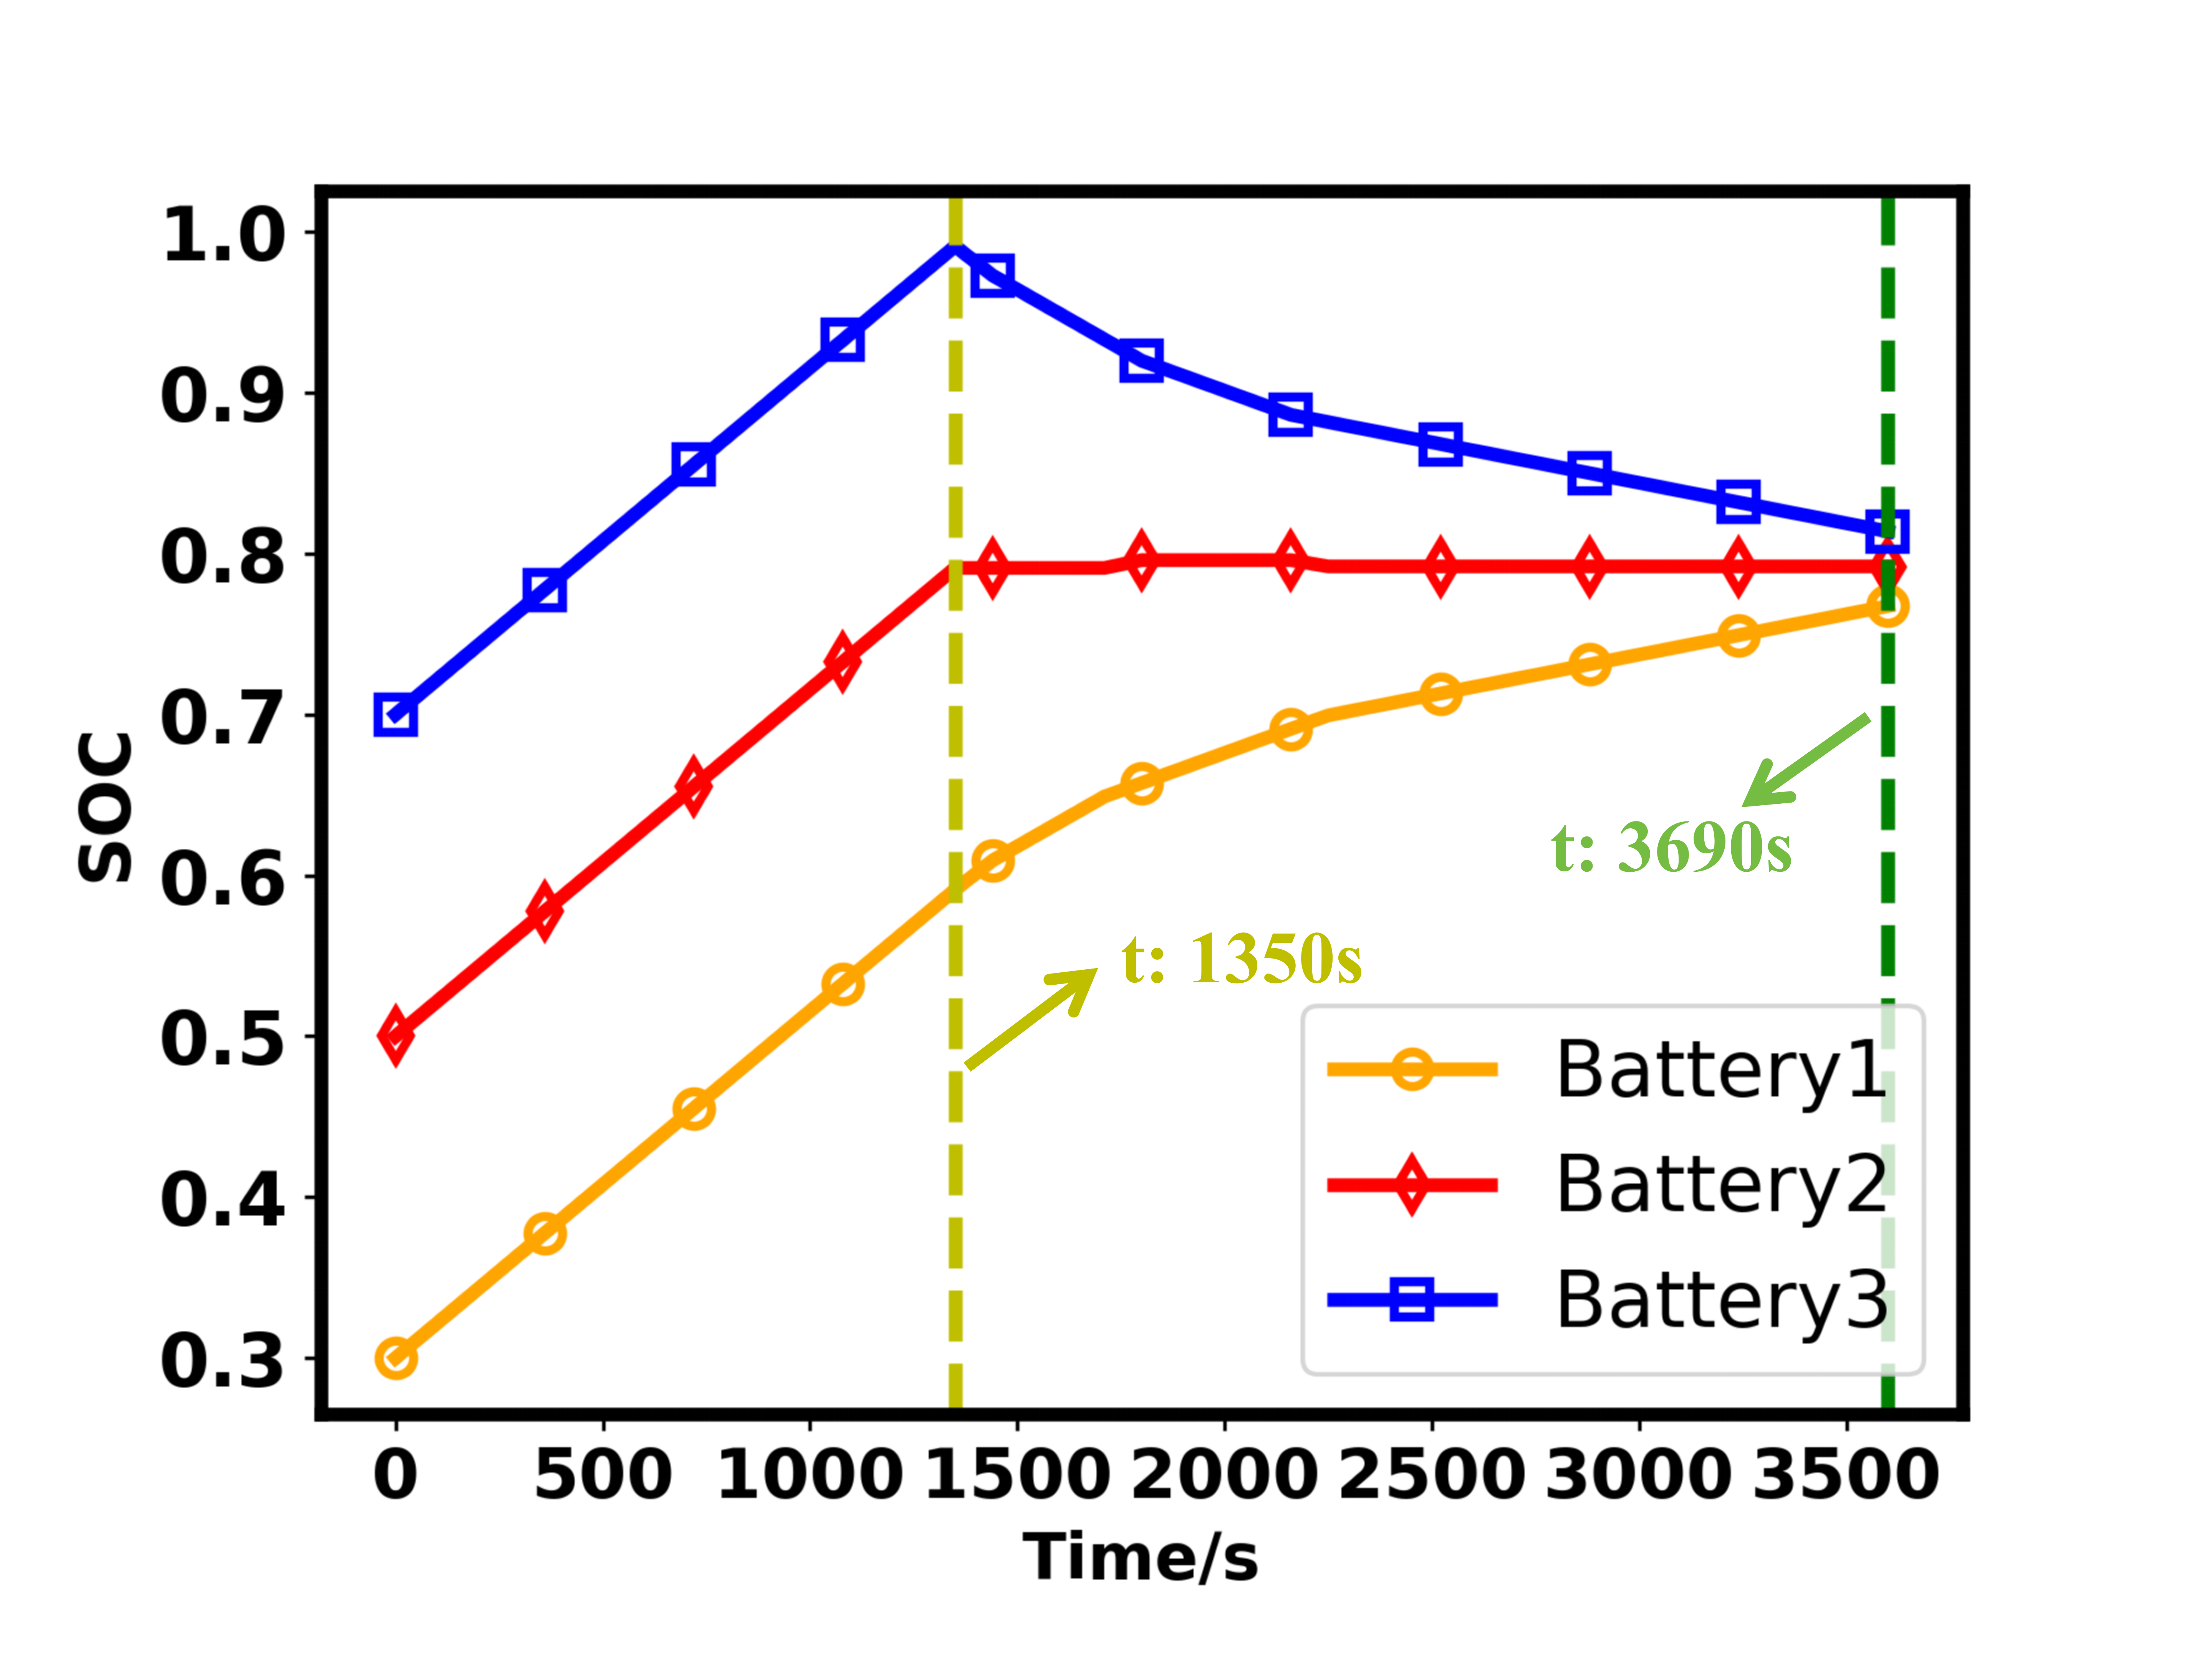
\includegraphics[width=\textwidth]{image/CC-CV 0.3 0.5 0.7.png}
        \caption{}
    \end{subfigure}

    \caption{Performance evaluations for MBA-RL, DQL, and CC-CV. The green dashed line indicates the time step at which balancing is reached, while the yellow dashed line marks the point at which the CC phase of the CC-CV charging protocol ends. (a) MBA-RL in $Set\;A$. (b) DQL in $Set\;A$. (c) CC-CV in $Set\;A$. (d) MBA-RL in $Set\;B$. (e) DQL in $Set\;B$. (f) CC-CV in $Set\;B$.}
    \label{fig:overall_figure}
\end{figure*}

\subsection{Parameter Identification for Batteries with Various Lifespans}
 To simulate battery aging, $Battery\;2$ and $Battery\;3$ underwent 140 and 260 charge-discharge cycles, respectively. The charging process followed a CC-CV protocol, beginning with a constant current charging at 2 C. Once the battery voltage reached 4.2 V, the charging transitioned to constant voltage mode, continuing until the current dropped to 0.1 C. The discharging process used a CC discharging at 1 C, and the discharging process was terminated when the voltage dropped to 2.5 V. Subsequently, the voltage and temperature data of the three batteries were recorded at a 1 C discharging current, as illustrated in Fig.~\ref{fig:three_aging}. The results clearly indicate that $Battery\;2$ and $Battery\;3$ exhibit noticeable signs of aging.

The PSO algorithm was chosen for parameter identification due to its gradient-free and fast convergence capability \cite{28}. Specifically, it minimizes the root mean squared error (RMSE) by aligning the voltage and temperature outputs of the simulated model with the experimentally measured data. Three independent experiments were conducted, and the results were subsequently averaged. The results of the parameter identification are presented in Figs.~\ref{battery1}-\ref{battery3}. The identification errors in voltage and temperature measurements for the three batteries are summarized in Table I. The RMSE values are all below 0.1, demonstrating a strong agreement between the simulated and measured data, thus confirming the effectiveness of the parameter identification process. This also ensures that the simulated SPM more closely reflects real-world battery behavior, reducing the gap between simulation results and actual conditions.


\begin{table}[t]
\centering
\caption{RMSEs for the three identified batteries}
\begin{tabular}{c c c c}
\noalign{\hrule height 0.3mm}
\textbf{} & $Battery1$ & $Battery2$ & $Battery3$ \\
\noalign{\hrule height 0.3mm}
$V_{RMSE}$ & 0.026 & 0.035 & 0.029 \\
\hline
$T_{RMSE}$ & 0.068 & 0.091 & 0.093 \\
\hline
\noalign{\hrule height 0.3mm}
\end{tabular}
\end{table}

\begin{table}[t]
\centering
\caption{Parameters of MBA-RL}
\begin{tabular}{c c}
\noalign{\hrule height 0.3mm}
\textbf{Parameters} & \textbf{Value} \\
\noalign{\hrule height 0.3mm}
Predefined threshold $\beta$ & 0.02 \\
\hline
The reference SOC $SOC_{ref}$ & 0.9 \\
\hline
The upper thresholds $T_{\text{max}}, V_{\text{max}}$ & 309, 4.2 \\
\hline
Learning rate $\alpha$ & 2e-4 \\
\hline
Number of episodes $N_{episode}$ & 1200 \\
\hline
Batch size $N$ & 128 \\
\hline
Target network update frequency $N_t$ & 50 \\
\hline
\noalign{\hrule height 0.3mm}
\end{tabular}
\end{table}

\begin{table}[t]
\centering
\caption{Battery pack's initial and terminal SOC vectors}
\label{tab:soc_vectors}
\begin{tabular}{c|c|c}
\hline
\noalign{\hrule height 0.2mm}
\textbf{Method} & \textbf{Initial SOC (\%)} & \textbf{Terminal SOC (\%)} \\ 
\hline
\noalign{\hrule height 0.2mm}
\multirow{2}{*}{MBA-RL} & $[10, 20, 30]^\text{T}$ & $[91.66, 94.18, 92.15]^\text{T}$ \\
                        & $[30, 50, 70]^\text{T}$ & $[91.23, 93.62, 91.41]^\text{T}$ \\ \hline
\multirow{2}{*}{DQL} & $[10, 20, 30]^\text{T}$ & $[24.72, 26.81, 28.05]^\text{T}$ \\
                        & $[30, 50, 70]^\text{T}$ & $[66.50, 69.18, 70.00]^\text{T}$ \\ \hline
\multirow{2}{*}{CC-CV}  & $[10, 20, 30]^\text{T}$ & $[52.41, 55.42, 56.97]^\text{T}$ \\
                        & $[30, 50, 70]^\text{T}$ & $[76.74, 79.21, 81.38]^\text{T}$ \\ \hline
                        \noalign{\hrule height 0.2mm}
\end{tabular}
\end{table}



\subsection{Performance Evaluation of MBA-RL}
We first constructed the battery model using the PyBaMM simulation platform \cite{29} and subsequently updated the model parameters with the identified values. All the experiments were conducted at an ambient temperature of 25 °C. In the comparison experiments, two sets of initial SOC values, $Set\; A = [10, 20, 30]^\text{T}$ and $Set\; B = [30, 50, 70]^\text{T}$, were selected for testing, as detailed in Table III. These sets highlight significant discrepancies in SOC across the battery pack, effectively emulating a real-world scenario where batteries typically exhibit inconsistent SOC distributions. In the experimental settings, the parameters of MBA-RL are detailed in Table II. The action space of MBA-RL was discretized from 0 to 7.5 A with increments of 0.5 A. Notably, the decision cycle of MBA-RL was set to 90 seconds, during which the selected actions remained unchanged. This configuration helps reduce the computational burden on the agent, as well as the complexity and time required during the training process. The action space of DQL consists of two components: determining the charging current for each battery and deciding when to adopt the cell-to-cell topology to facilitate the transfer of energy. The current range and decision cycle in DQL are consistent with those of MBA-RL. The reward function in DQL encompasses three key factors: charging time, balancing effectiveness, and charging safety. These factors are carefully balanced through a weighted approach, promoting the efficient convergence of the DQL algorithm. For the CC-CV method, the charging current during the CC stage is 4 A, and the voltage threshold for switching to the CV stage is 4 V. The termination condition for all three methods is the achievement of balance. As shown in Fig. 8 (a) and (d), to verify whether MBA-RL can optimize the charging trajectory while maintaining balance, we further investigated its performance after reaching the termination condition.

The balancing mode of MBA-RL operates at a current-level granularity. During each decision cycle, it dynamically adjusts the charging current based on the battery's state and the SOCs of the other batteries, ensuring that the output current allows multiple batteries to safely and rapidly reach balance. In contrast, DQL’s balancing mode determines the charging current for multiple batteries during each decision cycle and also decides whether to enable the cell-to-cell topology to facilitate energy transfer between cells. The balancing mode of CC-CV, on the other hand, activates the cell-to-cell topology when the CV phase begins and keeps it running until all batteries reach balance.

As shown in Fig.~\ref{fig:overall_figure}, we first compared the performance of DRL-based methods (i.e., MBA-RL and DQL) with the traditional CC-CV method for charging balancing control. The results revealed that the DRL-based methods significantly reduce the time required to achieve SOC balancing. Furthermore, the CC-CV employs a two-stage charging protocol, with balancing operations predominantly executed during the CV phase. This requires the completion of the CC phase before initiating balancing control, thereby considerably extending the overall balancing time. Moreover, during the phase transition in the CC-CV protocol, failure to account for safety constraints could result in issues such as overcharging or exceeding voltage and temperature safety thresholds, which may accelerate degradation and reduce the overall battery pack lifetime \cite{14, 17}. In contrast, the DRL-based methods effectively satisfy both safety and charging constraints while dynamically adapting to environmental changes. 

Subsequently, we analyzed the advantages of MBA-RL compared to the other two methods (i.e., DQL and CC-CV) from two perspectives. First, MBA-RL demonstrates a similar balancing time to DQL on $Set\; A$, being 1890 seconds faster than CC-CV. On $Set\; B$, it outperforms DQL by 270 seconds and CC-CV by 2520 seconds. A thorough analysis of the experimental results reveals that, despite a well-designed balancing algorithm (i.e., DQL) yielding excellent outcomes even when coupled with a simple topology (i.e., cell-to-cell), the issues of reduced control precision and efficiency due to the topology are inevitable. In contrast, MBA-RL effectively mitigates this problem by eliminating the need for an equalization topology, resulting in better balancing time and energy utilization efficiency compared to DQL. Moreover, MBA-RL achieves balancing control without discharging actions, effectively preventing the energy consumption associated with discharging. Second, MBA-RL simultaneously optimizes the balancing control for multiple batteries and the charging protocol for individual cells. It not only achieves effective balancing but also ensures that the SOC of the battery pack remains within the predefined threshold throughout the charging process, thereby preventing the recurrence of imbalance. In contrast, DQL and CC-CV separate the balancing and charging tasks. Once balancing is achieved, they continue to charge the batteries until the charging task is completed, which may lead to the reoccurrence of imbalance. In summary, the experimental results demonstrate that MBA-RL effectively addresses the inherent trade-offs among charging time, balancing speed, and safety constraints, resulting in a highly efficient and robust charging control system.


% unlike DQL and CC-CV, where the terminal SOC after balancing is significantly lower than the reference $SOC_{ref}$, potentially leading to the re-emergence of imbalance in subsequent charging cycles, MBA-RL not only achieves effective balancing but also ensures that the SOC of the battery pack remains within the predefined threshold throughout the charging process, thereby preventing the recurrence of imbalance. In summary, the experimental results demonstrate that MBA-RL effectively addresses the inherent trade-offs among charging time, balancing speed, and safety constraints, resulting in a highly efficient and robust charging control system.

% First, MBA-RL eliminates the need for an equalization topology in the balancing control process, effectively addressing issues of low energy utilization efficiency and imprecise charging caused by hardware constraints. Additionally, MBA-RL achieves balancing control without discharging actions, effectively preventing the energy consumption associated with discharging. Moreover, unlike DQL and CC-CV, where the terminal SOC after balancing is significantly lower than the reference $SOC_{ref}$, potentially leading to the re-emergence of imbalance in subsequent charging cycles, MBA-RL not only achieves effective balancing but also ensures that the SOC of the battery pack remains within the predefined threshold throughout the charging process, thereby preventing the recurrence of imbalance. In summary, the experimental results demonstrate that MBA-RL effectively addresses the inherent trade-offs among charging time, balancing speed, and safety constraints, resulting in a highly efficient and robust charging control system.

% As shown in Figs. 7(a) and (c), MBA-RL achieves balancing 1890 seconds faster than CC-CV, while also delivering an average terminal SOC that is 37.73\% higher upon reaching the termination conditions. Similarly, in Fig. 7(b), (d), MBA-RL reduces the balancing time by 2520 seconds and achieves an average terminal SOC that exceeds CC-CV by 12.98\%. These results highlight MBA-RL's ability to deliver faster and more effective balanced charging control. Additionally, MBA-RL offers several further advantages over CC-CV, which are analyzed below: 1) MBA-RL eliminates the need for a equalization topology to perform balancing control, thereby effectively avoiding the issue of low energy utilization efficiency caused by hardware structures; 2) MBA-RL achieves balancing control without discharging actions, effectively avoiding the energy consumption associated with discharging; 3) CC-CV's terminal SOC falls below $SOC_{ref}$ during the balancing process, which may lead to the re-emergence of imbalance in subsequent charging cycles. In contrast, MBA-RL not only achieves balancing but also maintains the battery pack's SOC within the predefined threshold in charging process, effectively preventing the recurrence of imbalance. Additionally, CC-CV employs a two-stage charging protocol, with balancing operations predominantly executed during the CV phase. This necessitates the completion of the CC phase prior to initiating balancing control, thereby significantly extending the overall balancing time. Moreover, during the phase transition in CC-CV protocol, the lack of consideration for safety constraints may lead to issues such as overcharging or exceeding voltage and temperature safety thresholds, potentially leading to accelerated degradation and reduced lifespan of the battery pack. The MBA-RL adeptly addresses the inherent trade-offs among charging time, balancing speed, and safety constraints, thereby achieving a highly efficient and robust charging control protocol.

\section{Conclusion}
In this paper, we present an MBA-RL charging control framework based on MARL to address the dual challenges of fast balancing and accelerated charging for lithium-ion batteries. The problem is systematically formulated as a Dec-POMDP, where the voltage, temperature, and SOC of each cell serve as the observations available to individual agents. Each agent is responsible for optimizing the charging protocol for its respective cell while coordinating the balancing control across all cells. By employing the MBA-RL charging control framework, the need for a dedicated equalization topology is eliminated, and discharging operations for high-SOC cells are effectively avoided. MBA-RL significantly improves energy utilization efficiency and charging precision. Furthermore, it facilitates rapid SOC balancing and enables all batteries to quickly reach the reference SOC under balanced conditions. This integrated charging and balancing mechanism ensures both speed and reliability across the charging process, making the framework highly suitable for deployment in diverse industrial applications. Moving forward, we aim to extend the validation of this method to large-scale battery systems, demonstrating its scalability and robustness.
\bibliographystyle{IEEEtran}
\bibliography{IEEEabrv,conf}


\iffalse
\begin{IEEEbiography}[{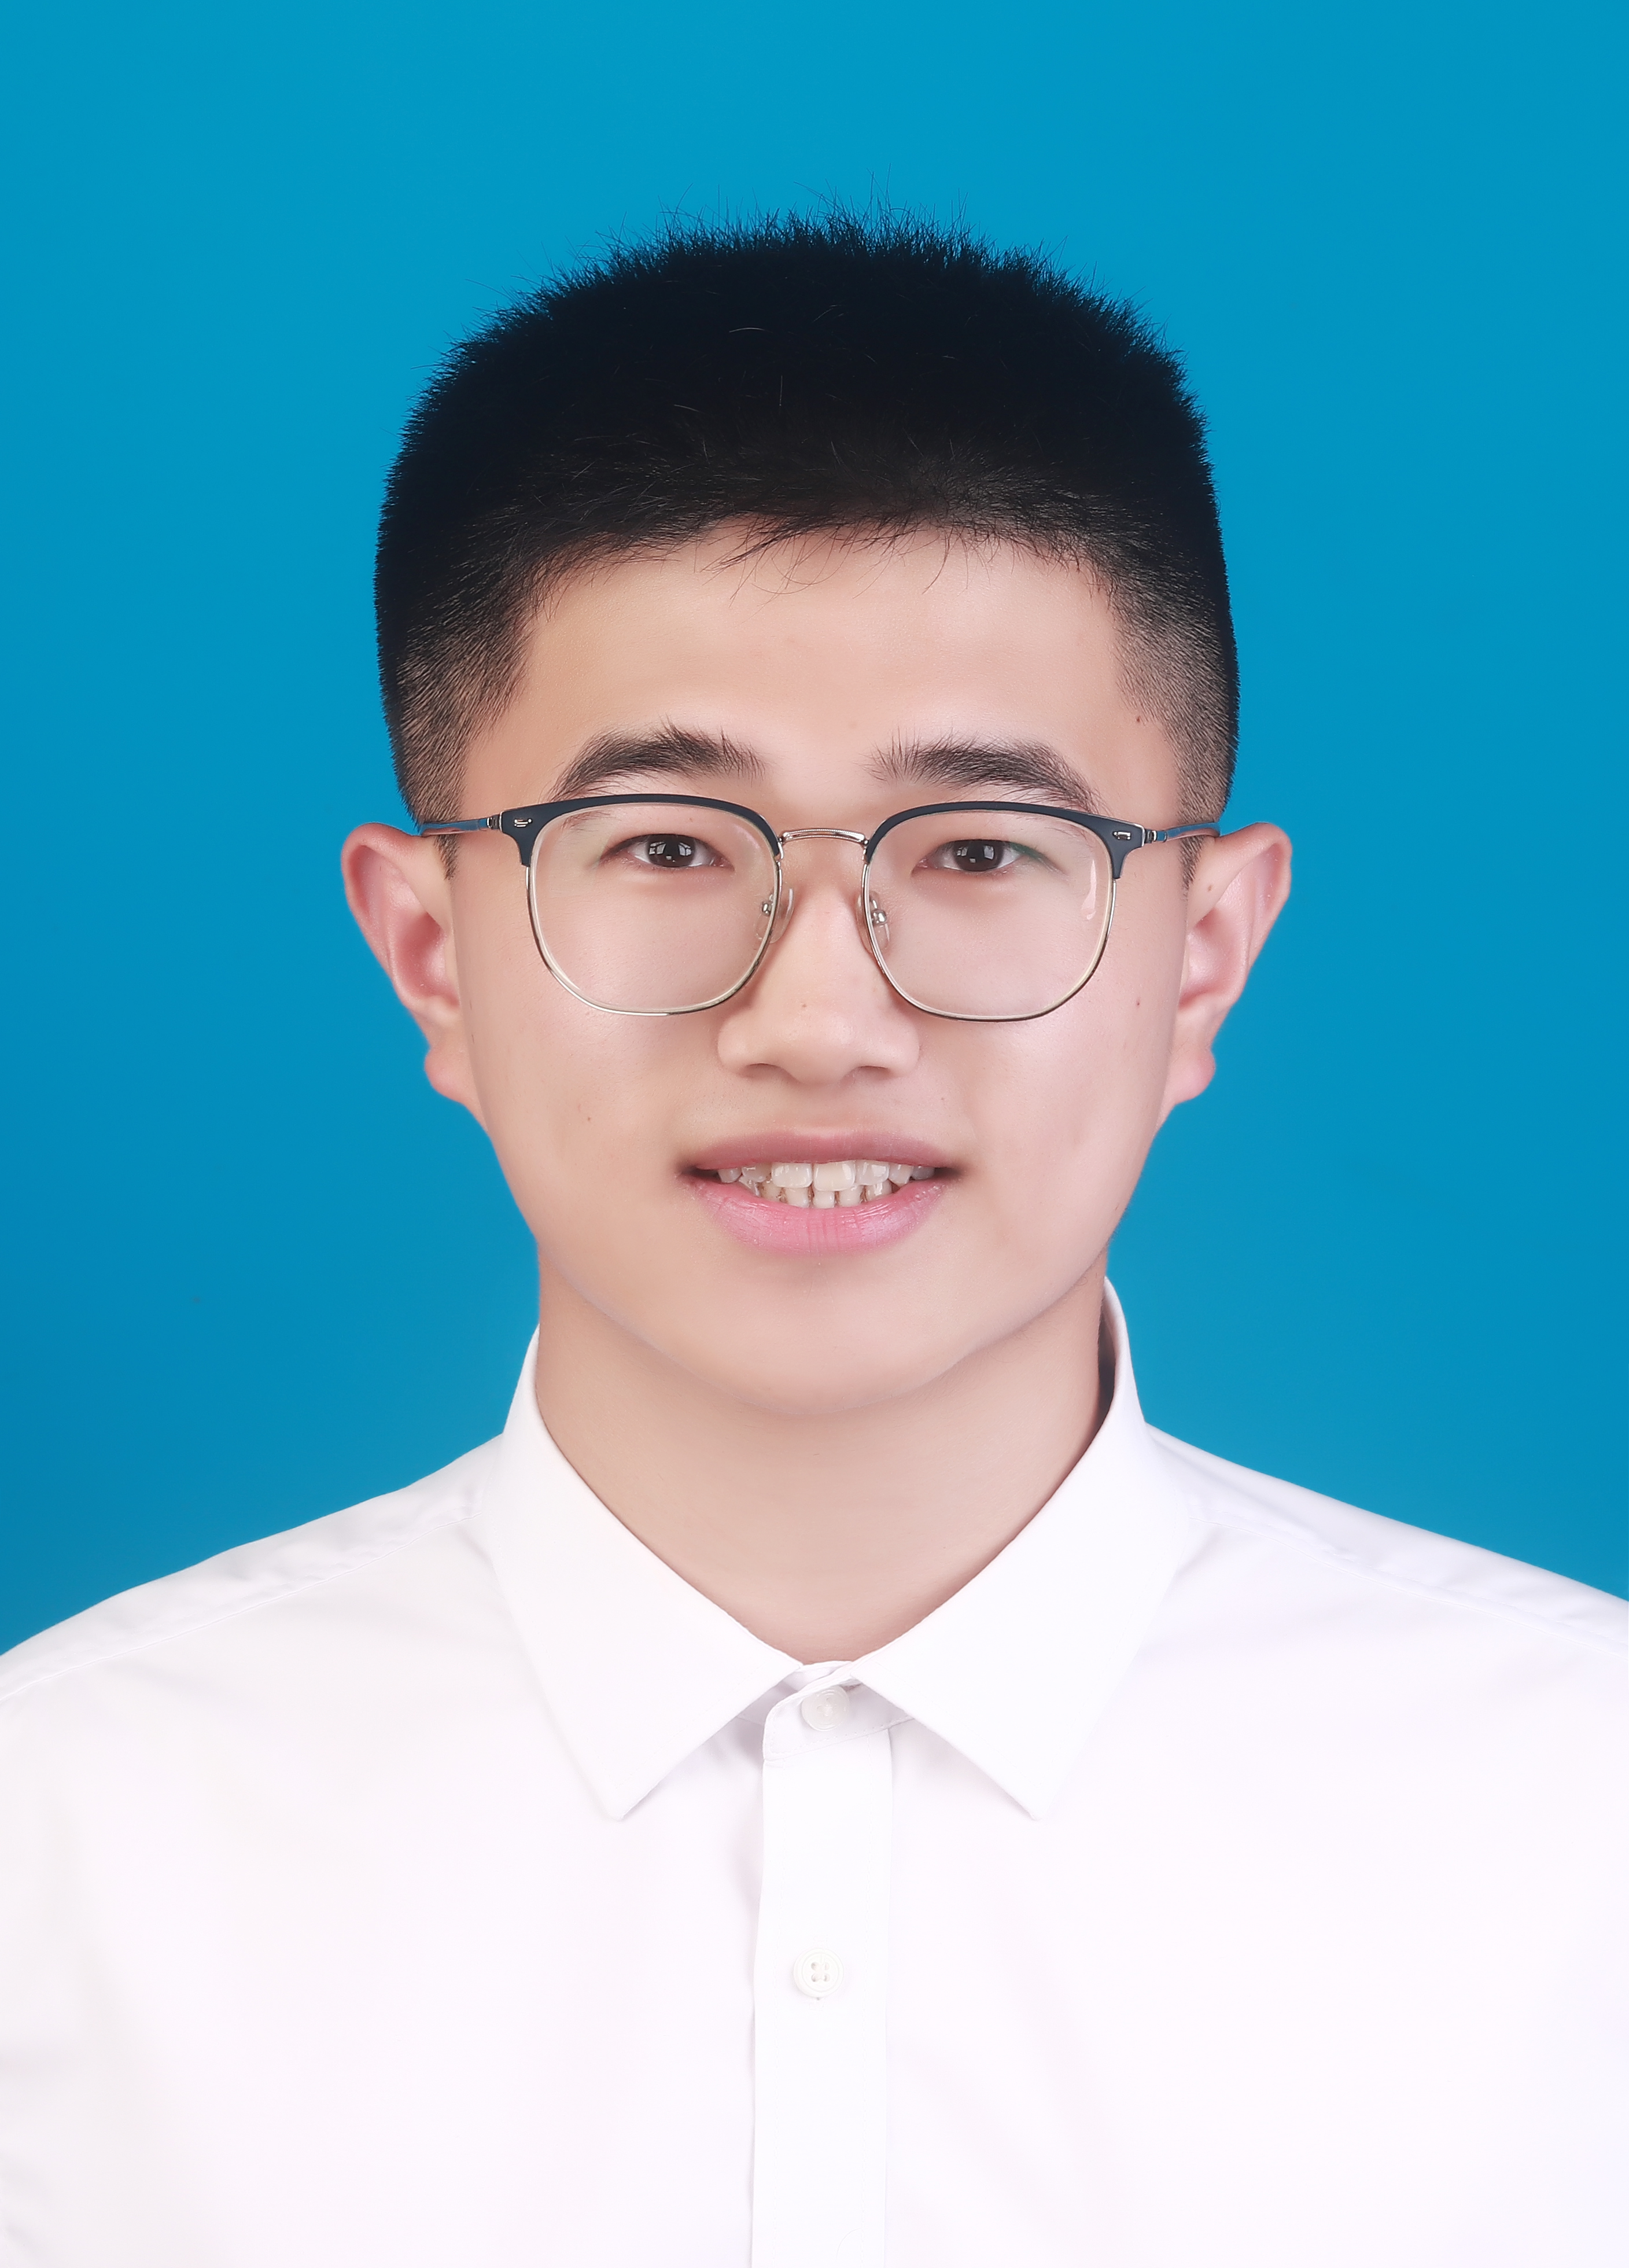
\includegraphics[width=1in,height=1.25in,clip,keepaspectratio]{image/CHJK.jpg}}]{Hejiakang Cao}
is working toward the undergraduate degree in artificial intelligence with the School of Automation, Central South University, Changsha, China. 

His research interests include reinforcement learning and its application to battery fast charging design and battery charging control.
\end{IEEEbiography}

\begin{IEEEbiography}[{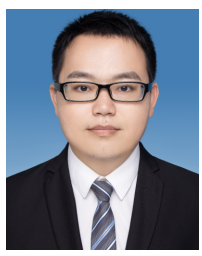
\includegraphics[width=1in,height=1.25in,clip,keepaspectratio]{image/Wang.png}}]{Bing-Chuan Wang}
(Member, IEEE) received the B.E. degree in automation and the M.S. degree in control science and engineering from the Central South University, Changsha, China, in 2013 and 2016, respectively, and the Ph.D. degree in system engineering and engineering management from The City University of Hong Kong, Hong Kong, in 2019. 

He is currently with the School of Automation, Central South University. His current research interests include computational intelligence and battery management systems.
\end{IEEEbiography}

\begin{IEEEbiography}[{
\includegraphics[width=1in,height=1.25in,clip,keepaspectratio]{image/Luo.png}}]{Biao Luo}
(Senior Member, IEEE) received the Ph.D. degree in control science and engineering from Beihang University, Beijing, China, in 2014. He is currently a Professor with the School of Automation, Central South University (CSU), Changsha, China. Before joining CSU, he was an Associate Professor and an Assistant Professor with the Institute of Automation, Chinese Academy of Sciences, Beijing, from 2014 to 2018. His current research interests include intelligent control, reinforcement learning, deep learning, and decisionmaking. 

Dr. Luo is the Vice-Chair of Adaptive Dynamic Programming and Reinforcement Learning Technical Committee and Chinese Association of Automation. He serves as an Associate Editor for \textit{IEEE TRANSACTIONS ON NEURAL NETWORKS AND LEARNING SYSTEMS}, the \textit{Artificial Intelligence Review}, the \textit{Neurocomputing}, and the \textit{Journal of Industrial and Management Optimization}.
\end{IEEEbiography}

\begin{IEEEbiography}[{
\includegraphics[width=1in,height=1.25in,clip,keepaspectratio]{image/Li.jpg}}]{Zhongmei Li}
(Member, IEEE) received the B.S. degree in automation and the M.S. and Ph.D. degrees in control science and engineering from Central South University, Changsha, China, in 2011, 2015, and 2019, respectively. 

From September 2017 to September 2019, she was a Visiting Scholar with New York University, New York, NY, USA. From January 2020 to July 2022, she held a post-doctoral position at the Key Laboratory of Smart Manufacturing in Energy Chemical Process, East China University of Science and Technology (ECUST), Shanghai, China. She currently works at ECUST. Her current research interests include data-driven optimal control, complex industrial process control, and adaptive dynamic programming. 

Dr. Li was a recipient of the 2023 IFAC Best Paper Prize and the 2020 IEEE CSS Beijing Chapter Young Author Prize.
\end{IEEEbiography}
\fi

\end{document}

% By leveraging the cooperation between the agent networks and the balancing network, lower currents are applied to batteries with higher SOC, while the maximum allowable current within safety limits is applied to batteries with lower SOC. Agents interact with batteries of varying initial SOC values to derive a generalized charge balancing strategy. 


% In QMIX, each agent $i$ has its own local stochastic policy $\pi^i \left( a_t^i \mid \tau^i \right)$, which makes decisions based on $o_t^i$ and $\tau^i$. The joint policy $\pi$ has a joint action-value function $Q^\pi(s_t, \mathbf{a_t})$, which describes the expected future discounted return given the state $s_t$ and the joint action $\mathbf{a_t}$:
% \begin{equation}
%     Q^\pi(s_t, \mathbf{a_t}) = \mathbb{E}_{s_{t+1:\infty}, \mathbf{a_{t+1:\infty}}} \left[ R_t \mid s_t, \mathbf{a_t} \right]
% \end{equation}
% where $R_t = \sum_{i=0}^{\infty} \gamma^i r_{t+i}$ indicates the expected cumulative discounted return.

% During design process, we utilize $Q_{tot}(\boldsymbol{\tau}, \mathbf{a}|\bm{\theta})$ to approximate $Q^\pi(s_t, \mathbf{a_t})$, where $\boldsymbol{\tau}$ denotes the joint action-observation history. Additionally, we employ $Q_i(\tau^i, a_t^i|\theta)$ to assess the efficacy of each agent’s actions, evaluating the expected return of executing action $a_t^i$ given the observation history $\tau^i$. This serves as a basis for guiding the optimization of the agent’s policy. It is crucial to emphasize that, to improve sample efficiency and strengthen the framework’s generalization capacity, all agents employ a unified set of parameters $\theta$. The objective of QMIX is to maximize the global Q-value $Q_{tot}(\boldsymbol{\tau}, \mathbf{a}|\bm{\theta})$. QMIX accomplishes this by decomposing the global Q-value into the Q-values of individual agents, while ensuring that the relationship between the global Q-value and each agent’s Q-value adheres to a monotonicity constraint. This constraint guarantees that maximizing each agent’s Q-value leads to the maximization of the global Q-value:
% \begin{equation}\label{QMIX_constraints}
% \arg\max_{\mathbf{a}} Q_{tot}(\boldsymbol{\tau}, \mathbf{a}|\bm{\theta}) =
% \begin{pmatrix}
% \arg\max_{a^1} Q_1(\tau^1, a^1|\theta) \\
% \vdots \\
% \arg\max_{a^n} Q_n(\tau^n, a^n|\theta)
% \end{pmatrix}
% \end{equation}
% where \eqref{QMIX_constraints} enables each agent $i$ to greedily select the action that maximize $Q_i(\tau^i, a_t^i|\theta)$ for decentralized execution.

% For each agent $i$, the agent network is modeled as a deep recurrent Q-network (DRQN), which integrates the current observation $o_t^i$ at each time step with the previous action $a_{t-1}^i$ to construct the action-observation history $\tau^i$. Each agent chooses current action $a_t^i$ using the $\epsilon$-greedy strategy, which can be described as follows:
% \begin{equation}\label{epsilon-greedy}
% a_t^i =
% \begin{cases}
% \text{random action} & \text{with probability } \epsilon \\
% \arg\max_{a_t^i} Q_i(\tau^i, a_t^i|\theta) & \text{with probability } 1 - \epsilon
% \end{cases}
% \end{equation}
% then $Q_i(\tau^i, a_t^i|\theta)$ is computed based on the $\tau^i$ and the $a_t^i$.

% The mixing network is a feed-forward neural network that receives the outputs of all agent networks as input and combines them monotonically, generating the values of $Q_{tot}(\boldsymbol{\tau}, \mathbf{a}|\bm{\theta})$:
% \begin{equation}\label{Q-value}
%     Q_{tot}(\boldsymbol{\tau}, \mathbf{a}|\bm{\theta}) = f(Q_1(\tau^1, a_t^1|\theta), ..., Q_n(\tau^n, a_t^n|\theta), s_t).
% \end{equation}

% The mixing network’s weights are generated by distinct hypernetworks. Each hypernetwork receives the state $s_t$ as input and outputs the weights for a specific layer of the mixing network. To enforce \eqref{QMIX_constraints}, the weights of the mixing network are strictly constrained to be non-negative:
% \begin{equation}
% \frac{\partial Q_{tot}}{\partial Q_i} \geq 0, \, i = 1, 2, ..., n.
% \end{equation}